% Options for packages loaded elsewhere
\PassOptionsToPackage{unicode}{hyperref}
\PassOptionsToPackage{hyphens}{url}
\PassOptionsToPackage{dvipsnames,svgnames,x11names}{xcolor}
%
\documentclass[
  letterpaper,
  DIV=11,
  numbers=noendperiod]{scrartcl}

\usepackage{amsmath,amssymb}
\usepackage{iftex}
\ifPDFTeX
  \usepackage[T1]{fontenc}
  \usepackage[utf8]{inputenc}
  \usepackage{textcomp} % provide euro and other symbols
\else % if luatex or xetex
  \usepackage{unicode-math}
  \defaultfontfeatures{Scale=MatchLowercase}
  \defaultfontfeatures[\rmfamily]{Ligatures=TeX,Scale=1}
\fi
\usepackage{lmodern}
\ifPDFTeX\else  
    % xetex/luatex font selection
\fi
% Use upquote if available, for straight quotes in verbatim environments
\IfFileExists{upquote.sty}{\usepackage{upquote}}{}
\IfFileExists{microtype.sty}{% use microtype if available
  \usepackage[]{microtype}
  \UseMicrotypeSet[protrusion]{basicmath} % disable protrusion for tt fonts
}{}
\makeatletter
\@ifundefined{KOMAClassName}{% if non-KOMA class
  \IfFileExists{parskip.sty}{%
    \usepackage{parskip}
  }{% else
    \setlength{\parindent}{0pt}
    \setlength{\parskip}{6pt plus 2pt minus 1pt}}
}{% if KOMA class
  \KOMAoptions{parskip=half}}
\makeatother
\usepackage{xcolor}
\setlength{\emergencystretch}{3em} % prevent overfull lines
\setcounter{secnumdepth}{-\maxdimen} % remove section numbering
% Make \paragraph and \subparagraph free-standing
\ifx\paragraph\undefined\else
  \let\oldparagraph\paragraph
  \renewcommand{\paragraph}[1]{\oldparagraph{#1}\mbox{}}
\fi
\ifx\subparagraph\undefined\else
  \let\oldsubparagraph\subparagraph
  \renewcommand{\subparagraph}[1]{\oldsubparagraph{#1}\mbox{}}
\fi

\usepackage{color}
\usepackage{fancyvrb}
\newcommand{\VerbBar}{|}
\newcommand{\VERB}{\Verb[commandchars=\\\{\}]}
\DefineVerbatimEnvironment{Highlighting}{Verbatim}{commandchars=\\\{\}}
% Add ',fontsize=\small' for more characters per line
\usepackage{framed}
\definecolor{shadecolor}{RGB}{241,243,245}
\newenvironment{Shaded}{\begin{snugshade}}{\end{snugshade}}
\newcommand{\AlertTok}[1]{\textcolor[rgb]{0.68,0.00,0.00}{#1}}
\newcommand{\AnnotationTok}[1]{\textcolor[rgb]{0.37,0.37,0.37}{#1}}
\newcommand{\AttributeTok}[1]{\textcolor[rgb]{0.40,0.45,0.13}{#1}}
\newcommand{\BaseNTok}[1]{\textcolor[rgb]{0.68,0.00,0.00}{#1}}
\newcommand{\BuiltInTok}[1]{\textcolor[rgb]{0.00,0.23,0.31}{#1}}
\newcommand{\CharTok}[1]{\textcolor[rgb]{0.13,0.47,0.30}{#1}}
\newcommand{\CommentTok}[1]{\textcolor[rgb]{0.37,0.37,0.37}{#1}}
\newcommand{\CommentVarTok}[1]{\textcolor[rgb]{0.37,0.37,0.37}{\textit{#1}}}
\newcommand{\ConstantTok}[1]{\textcolor[rgb]{0.56,0.35,0.01}{#1}}
\newcommand{\ControlFlowTok}[1]{\textcolor[rgb]{0.00,0.23,0.31}{#1}}
\newcommand{\DataTypeTok}[1]{\textcolor[rgb]{0.68,0.00,0.00}{#1}}
\newcommand{\DecValTok}[1]{\textcolor[rgb]{0.68,0.00,0.00}{#1}}
\newcommand{\DocumentationTok}[1]{\textcolor[rgb]{0.37,0.37,0.37}{\textit{#1}}}
\newcommand{\ErrorTok}[1]{\textcolor[rgb]{0.68,0.00,0.00}{#1}}
\newcommand{\ExtensionTok}[1]{\textcolor[rgb]{0.00,0.23,0.31}{#1}}
\newcommand{\FloatTok}[1]{\textcolor[rgb]{0.68,0.00,0.00}{#1}}
\newcommand{\FunctionTok}[1]{\textcolor[rgb]{0.28,0.35,0.67}{#1}}
\newcommand{\ImportTok}[1]{\textcolor[rgb]{0.00,0.46,0.62}{#1}}
\newcommand{\InformationTok}[1]{\textcolor[rgb]{0.37,0.37,0.37}{#1}}
\newcommand{\KeywordTok}[1]{\textcolor[rgb]{0.00,0.23,0.31}{#1}}
\newcommand{\NormalTok}[1]{\textcolor[rgb]{0.00,0.23,0.31}{#1}}
\newcommand{\OperatorTok}[1]{\textcolor[rgb]{0.37,0.37,0.37}{#1}}
\newcommand{\OtherTok}[1]{\textcolor[rgb]{0.00,0.23,0.31}{#1}}
\newcommand{\PreprocessorTok}[1]{\textcolor[rgb]{0.68,0.00,0.00}{#1}}
\newcommand{\RegionMarkerTok}[1]{\textcolor[rgb]{0.00,0.23,0.31}{#1}}
\newcommand{\SpecialCharTok}[1]{\textcolor[rgb]{0.37,0.37,0.37}{#1}}
\newcommand{\SpecialStringTok}[1]{\textcolor[rgb]{0.13,0.47,0.30}{#1}}
\newcommand{\StringTok}[1]{\textcolor[rgb]{0.13,0.47,0.30}{#1}}
\newcommand{\VariableTok}[1]{\textcolor[rgb]{0.07,0.07,0.07}{#1}}
\newcommand{\VerbatimStringTok}[1]{\textcolor[rgb]{0.13,0.47,0.30}{#1}}
\newcommand{\WarningTok}[1]{\textcolor[rgb]{0.37,0.37,0.37}{\textit{#1}}}

\providecommand{\tightlist}{%
  \setlength{\itemsep}{0pt}\setlength{\parskip}{0pt}}\usepackage{longtable,booktabs,array}
\usepackage{calc} % for calculating minipage widths
% Correct order of tables after \paragraph or \subparagraph
\usepackage{etoolbox}
\makeatletter
\patchcmd\longtable{\par}{\if@noskipsec\mbox{}\fi\par}{}{}
\makeatother
% Allow footnotes in longtable head/foot
\IfFileExists{footnotehyper.sty}{\usepackage{footnotehyper}}{\usepackage{footnote}}
\makesavenoteenv{longtable}
\usepackage{graphicx}
\makeatletter
\def\maxwidth{\ifdim\Gin@nat@width>\linewidth\linewidth\else\Gin@nat@width\fi}
\def\maxheight{\ifdim\Gin@nat@height>\textheight\textheight\else\Gin@nat@height\fi}
\makeatother
% Scale images if necessary, so that they will not overflow the page
% margins by default, and it is still possible to overwrite the defaults
% using explicit options in \includegraphics[width, height, ...]{}
\setkeys{Gin}{width=\maxwidth,height=\maxheight,keepaspectratio}
% Set default figure placement to htbp
\makeatletter
\def\fps@figure{htbp}
\makeatother

\usepackage{booktabs}
\usepackage{longtable}
\usepackage{array}
\usepackage{multirow}
\usepackage{wrapfig}
\usepackage{float}
\usepackage{colortbl}
\usepackage{pdflscape}
\usepackage{tabu}
\usepackage{threeparttable}
\usepackage{threeparttablex}
\usepackage[normalem]{ulem}
\usepackage{makecell}
\usepackage{xcolor}
\KOMAoption{captions}{tableheading}
\makeatletter
\makeatother
\makeatletter
\makeatother
\makeatletter
\@ifpackageloaded{caption}{}{\usepackage{caption}}
\AtBeginDocument{%
\ifdefined\contentsname
  \renewcommand*\contentsname{Table of contents}
\else
  \newcommand\contentsname{Table of contents}
\fi
\ifdefined\listfigurename
  \renewcommand*\listfigurename{List of Figures}
\else
  \newcommand\listfigurename{List of Figures}
\fi
\ifdefined\listtablename
  \renewcommand*\listtablename{List of Tables}
\else
  \newcommand\listtablename{List of Tables}
\fi
\ifdefined\figurename
  \renewcommand*\figurename{Figure}
\else
  \newcommand\figurename{Figure}
\fi
\ifdefined\tablename
  \renewcommand*\tablename{Table}
\else
  \newcommand\tablename{Table}
\fi
}
\@ifpackageloaded{float}{}{\usepackage{float}}
\floatstyle{ruled}
\@ifundefined{c@chapter}{\newfloat{codelisting}{h}{lop}}{\newfloat{codelisting}{h}{lop}[chapter]}
\floatname{codelisting}{Listing}
\newcommand*\listoflistings{\listof{codelisting}{List of Listings}}
\makeatother
\makeatletter
\@ifpackageloaded{caption}{}{\usepackage{caption}}
\@ifpackageloaded{subcaption}{}{\usepackage{subcaption}}
\makeatother
\makeatletter
\@ifpackageloaded{tcolorbox}{}{\usepackage[skins,breakable]{tcolorbox}}
\makeatother
\makeatletter
\@ifundefined{shadecolor}{\definecolor{shadecolor}{rgb}{.97, .97, .97}}
\makeatother
\makeatletter
\makeatother
\makeatletter
\makeatother
\ifLuaTeX
  \usepackage{selnolig}  % disable illegal ligatures
\fi
\IfFileExists{bookmark.sty}{\usepackage{bookmark}}{\usepackage{hyperref}}
\IfFileExists{xurl.sty}{\usepackage{xurl}}{} % add URL line breaks if available
\urlstyle{same} % disable monospaced font for URLs
\hypersetup{
  pdftitle={Favipiravir PLATCOV},
  pdfauthor={James Watson},
  colorlinks=true,
  linkcolor={blue},
  filecolor={Maroon},
  citecolor={Blue},
  urlcolor={Blue},
  pdfcreator={LaTeX via pandoc}}

\title{Favipiravir PLATCOV}
\author{James Watson}
\date{}

\begin{document}
\maketitle
\ifdefined\Shaded\renewenvironment{Shaded}{\begin{tcolorbox}[enhanced, boxrule=0pt, borderline west={3pt}{0pt}{shadecolor}, interior hidden, frame hidden, sharp corners, breakable]}{\end{tcolorbox}}\fi

\begin{Shaded}
\begin{Highlighting}[]
\NormalTok{knitr}\SpecialCharTok{::}\NormalTok{opts\_chunk}\SpecialCharTok{$}\FunctionTok{set}\NormalTok{(}\AttributeTok{cache =}\NormalTok{ T, }\AttributeTok{cache.comments =} \ConstantTok{FALSE}\NormalTok{,}
                      \AttributeTok{echo =}\NormalTok{ F, }\AttributeTok{include =} \ConstantTok{TRUE}\NormalTok{, }
                      \AttributeTok{fig.width =} \DecValTok{8}\NormalTok{, }\AttributeTok{fig.height =} \DecValTok{8}\NormalTok{,}
                      \AttributeTok{fig.pos =} \StringTok{\textquotesingle{}H\textquotesingle{}}\NormalTok{,}\AttributeTok{dev =} \StringTok{\textquotesingle{}png\textquotesingle{}}\NormalTok{, }\AttributeTok{dpi =} \DecValTok{300}\NormalTok{)}
\end{Highlighting}
\end{Shaded}

\begin{verbatim}
Loading required package: StanHeaders
\end{verbatim}

\begin{verbatim}

rstan version 2.26.22 (Stan version 2.26.1)
\end{verbatim}

\begin{verbatim}
For execution on a local, multicore CPU with excess RAM we recommend calling
options(mc.cores = parallel::detectCores()).
To avoid recompilation of unchanged Stan programs, we recommend calling
rstan_options(auto_write = TRUE)
For within-chain threading using `reduce_sum()` or `map_rect()` Stan functions,
change `threads_per_chain` option:
rstan_options(threads_per_chain = 1)
\end{verbatim}

\begin{verbatim}
Do not specify '-march=native' in 'LOCAL_CPPFLAGS' or a Makevars file
\end{verbatim}

\begin{verbatim}
-- Attaching core tidyverse packages ------------------------ tidyverse 2.0.0 --
v dplyr     1.1.2     v readr     2.1.4
v forcats   1.0.0     v stringr   1.5.0
v ggplot2   3.4.3     v tibble    3.2.1
v lubridate 1.9.2     v tidyr     1.3.0
v purrr     1.0.1     
-- Conflicts ------------------------------------------ tidyverse_conflicts() --
x tidyr::extract() masks rstan::extract()
x dplyr::filter()  masks stats::filter()
x dplyr::lag()     masks stats::lag()
i Use the conflicted package (<http://conflicted.r-lib.org/>) to force all conflicts to become errors

Attaching package: 'kableExtra'


The following object is masked from 'package:dplyr':

    group_rows
\end{verbatim}

\begin{verbatim}
               _                                
platform       x86_64-w64-mingw32               
arch           x86_64                           
os             mingw32                          
crt            ucrt                             
system         x86_64, mingw32                  
status                                          
major          4                                
minor          3.1                              
year           2023                             
month          06                               
day            16                               
svn rev        84548                            
language       R                                
version.string R version 4.3.1 (2023-06-16 ucrt)
nickname       Beagle Scouts                    
\end{verbatim}

\begin{verbatim}
R version 4.3.1 (2023-06-16 ucrt)
Platform: x86_64-w64-mingw32/x64 (64-bit)
Running under: Windows 11 x64 (build 22621)

Matrix products: default


locale:
[1] LC_COLLATE=English_United States.utf8 
[2] LC_CTYPE=English_United States.utf8   
[3] LC_MONETARY=English_United States.utf8
[4] LC_NUMERIC=C                          
[5] LC_TIME=English_United States.utf8    

time zone: Asia/Bangkok
tzcode source: internal

attached base packages:
[1] stats     graphics  grDevices utils     datasets  methods   base     

other attached packages:
 [1] RColorBrewer_1.1-3  finalfit_1.0.6      kableExtra_1.3.4   
 [4] lubridate_1.9.2     forcats_1.0.0       stringr_1.5.0      
 [7] dplyr_1.1.2         purrr_1.0.1         readr_2.1.4        
[10] tidyr_1.3.0         tibble_3.2.1        ggplot2_3.4.3      
[13] tidyverse_2.0.0     rstan_2.26.22       StanHeaders_2.26.27

loaded via a namespace (and not attached):
 [1] tidyselect_1.2.0   viridisLite_0.4.2  loo_2.6.0          fastmap_1.1.1     
 [5] rpart_4.1.19       digest_0.6.33      timechange_0.2.0   lifecycle_1.0.3   
 [9] survival_3.5-5     processx_3.8.2     magrittr_2.0.3     compiler_4.3.1    
[13] rlang_1.1.1        tools_4.3.1        utf8_1.2.3         yaml_2.3.7        
[17] knitr_1.43         prettyunits_1.1.1  pkgbuild_1.4.2     curl_5.0.1        
[21] xml2_1.3.5         withr_2.5.0        nnet_7.3-19        grid_4.3.1        
[25] stats4_4.3.1       fansi_1.0.4        jomo_2.7-6         colorspace_2.1-0  
[29] mice_3.16.0        inline_0.3.19      scales_1.2.1       iterators_1.0.14  
[33] MASS_7.3-60        cli_3.6.1          rmarkdown_2.23     crayon_1.5.2      
[37] generics_0.1.3     RcppParallel_5.1.7 rstudioapi_0.15.0  httr_1.4.6        
[41] tzdb_0.4.0         minqa_1.2.5        splines_4.3.1      rvest_1.0.3       
[45] parallel_4.3.1     matrixStats_1.0.0  vctrs_0.6.3        V8_4.3.3          
[49] boot_1.3-28.1      glmnet_4.1-7       webshot_0.5.5      Matrix_1.6-0      
[53] jsonlite_1.8.7     callr_3.7.3        hms_1.1.3          mitml_0.4-5       
[57] systemfonts_1.0.4  foreach_1.5.2      glue_1.6.2         pan_1.8           
[61] nloptr_2.0.3       codetools_0.2-19   ps_1.7.5           stringi_1.7.12    
[65] gtable_0.3.3       shape_1.4.6        lme4_1.1-34        munsell_0.5.0     
[69] pillar_1.9.0       htmltools_0.5.6    R6_2.5.1           evaluate_0.21     
[73] lattice_0.21-8     backports_1.4.1    broom_1.0.5        Rcpp_1.0.11       
[77] nlme_3.1-162       svglite_2.1.1      gridExtra_2.3      xfun_0.39         
[81] pkgconfig_2.0.3   
\end{verbatim}

\begin{verbatim}
Warning in checkStrict(plot_serial_data): global variables used: daily_VL, ID,
log10_viral_load, Time, Timepoint_ID, Trt, trt_color
\end{verbatim}

\begin{verbatim}
Warning in checkStrict(calculate_fever_clearance): global variables used: ID,
Time
\end{verbatim}

\hypertarget{load-data}{%
\subsection{Load data}\label{load-data}}

Set up analysis

\begin{verbatim}
Missing patients in No study drug arm:
Missing patients in Fluoxetine arm:
\end{verbatim}

\begin{verbatim}
[1] "PLT-BR3-048" "PLT-BR3-088" "PLT-TH1-185"
\end{verbatim}

\begin{verbatim}
[1] "Fluoxetine"    "Fluoxetine"    "No study drug"
\end{verbatim}

\hypertarget{make-modified-intention-to-treat-population}{%
\subsection{Make modified intention to treat
population}\label{make-modified-intention-to-treat-population}}

\begin{verbatim}
               mITT population
Intervention    FALSE TRUE
  Fluoxetine        2  116
  No study drug     1  150
\end{verbatim}

\hypertarget{baseline-characteristics}{%
\subsection{Baseline characteristics}\label{baseline-characteristics}}

\begin{verbatim}
Warning: There was 1 warning in `mutate()`.
i In argument: `Site = (function (f, na_level = "(Missing)") ...`.
Caused by warning:
! `fct_explicit_na()` was deprecated in forcats 1.0.0.
i Please use `fct_na_value_to_level()` instead.
i The deprecated feature was likely used in the dplyr package.
  Please report the issue at <https://github.com/tidyverse/dplyr/issues>.
\end{verbatim}

\begin{table}

\caption{Baseline characteristics in mITT population}
\centering
\begin{tabular}[t]{lrlrr}
\toprule
Dependent: Trt &   & No study drug & Fluoxetine & Total\\
\midrule
Site & br003 & 17 (11.3) & 12 (10.3) & 29 (10.9)\\
 & la008 & 0 (0.0) & 1 (0.9) & 1 (0.4)\\
 & pk001 & 4 (2.7) & 2 (1.7) & 6 (2.3)\\
 & th001 & 129 (86.0) & 101 (87.1) & 230 (86.5)\\
Age & Mean (SD) & 30.5 (7.8) & 29.5 (7.7) & 30.1 (7.8)\\
\addlinespace
Sex & Male & 52 (34.7) & 34 (29.3) & 86 (32.3)\\
 & Female & 98 (65.3) & 82 (70.7) & 180 (67.7)\\
BMI & Mean (SD) & 23.2 (4.0) & 22.3 (3.5) & 22.8 (3.8)\\
Weight & Mean (SD) & 62.7 (13.4) & 59.6 (11.3) & 61.4 (12.6)\\
Baseline.viral.load & Mean (SD) & 5.5 (1.4) & 5.6 (1.3) & 5.5 (1.3)\\
\addlinespace
Variant & BA.2 & 30 (20.0) & 25 (21.6) & 55 (20.7)\\
 & BA.5 & 41 (27.3) & 29 (25.0) & 70 (26.3)\\
 & BA.2.75 & 43 (28.7) & 34 (29.3) & 77 (28.9)\\
 & XBB & 10 (6.7) & 9 (7.8) & 19 (7.1)\\
 & BA.4 & 2 (1.3) & 0 (0.0) & 2 (0.8)\\
\addlinespace
 & BQ.1 & 1 (0.7) & 2 (1.7) & 3 (1.1)\\
 & XBB.1.5-like & 21 (14.0) & 14 (12.1) & 35 (13.2)\\
 & - & 0 (0.0) & 2 (1.7) & 2 (0.8)\\
 & FL.4 & 1 (0.7) & 1 (0.9) & 2 (0.8)\\
 & EG.2 & 1 (0.7) & 0 (0.0) & 1 (0.4)\\
\addlinespace
Symptom\_onset & Mean (SD) & 2.1 (0.8) & 2.1 (0.8) & 2.1 (0.8)\\
Vaccinated & Yes & 150 (100.0) & 116 (100.0) & 266 (100.0)\\
 & No & 0 (0.0) & 0 (0.0) & 0 (0.0)\\
Fever\_Baseline & 0 & 115 (76.7) & 85 (73.3) & 200 (75.2)\\
 & 1 & 35 (23.3) & 31 (26.7) & 66 (24.8)\\
\bottomrule
\end{tabular}
\end{table}

\hypertarget{fit-models}{%
\subsection{Fit models}\label{fit-models}}

\begin{verbatim}
Analysis dataset contains 266 patients and 3718 datapoints (3338 above LLOD, 90%)
\end{verbatim}

\begin{verbatim}
There are a total of 266 patients in the database with a total of 3718 PCRs analysable
10.22% of samples are below LOD
check stan data formatting:
\end{verbatim}

\begin{verbatim}
We are running all models with 4 chains and 2000 samples for each chain, discarding 1000 for burn-in and thining every 4, thus giving a total of 1000 posterior samples per model.
\end{verbatim}

main model selection

\begin{verbatim}
Warning in brewer.pal(n = nrow(model_settings), name = "Set1"): minimal value for n is 3, returning requested palette with 3 different levels
\end{verbatim}

\hypertarget{plot-treatment-effect}{%
\section{Plot treatment effect}\label{plot-treatment-effect}}

\begin{verbatim}
`summarise()` has grouped output by 'Timepoint_ID'. You can override using the
`.groups` argument.
\end{verbatim}

\begin{figure}[H]

{\centering 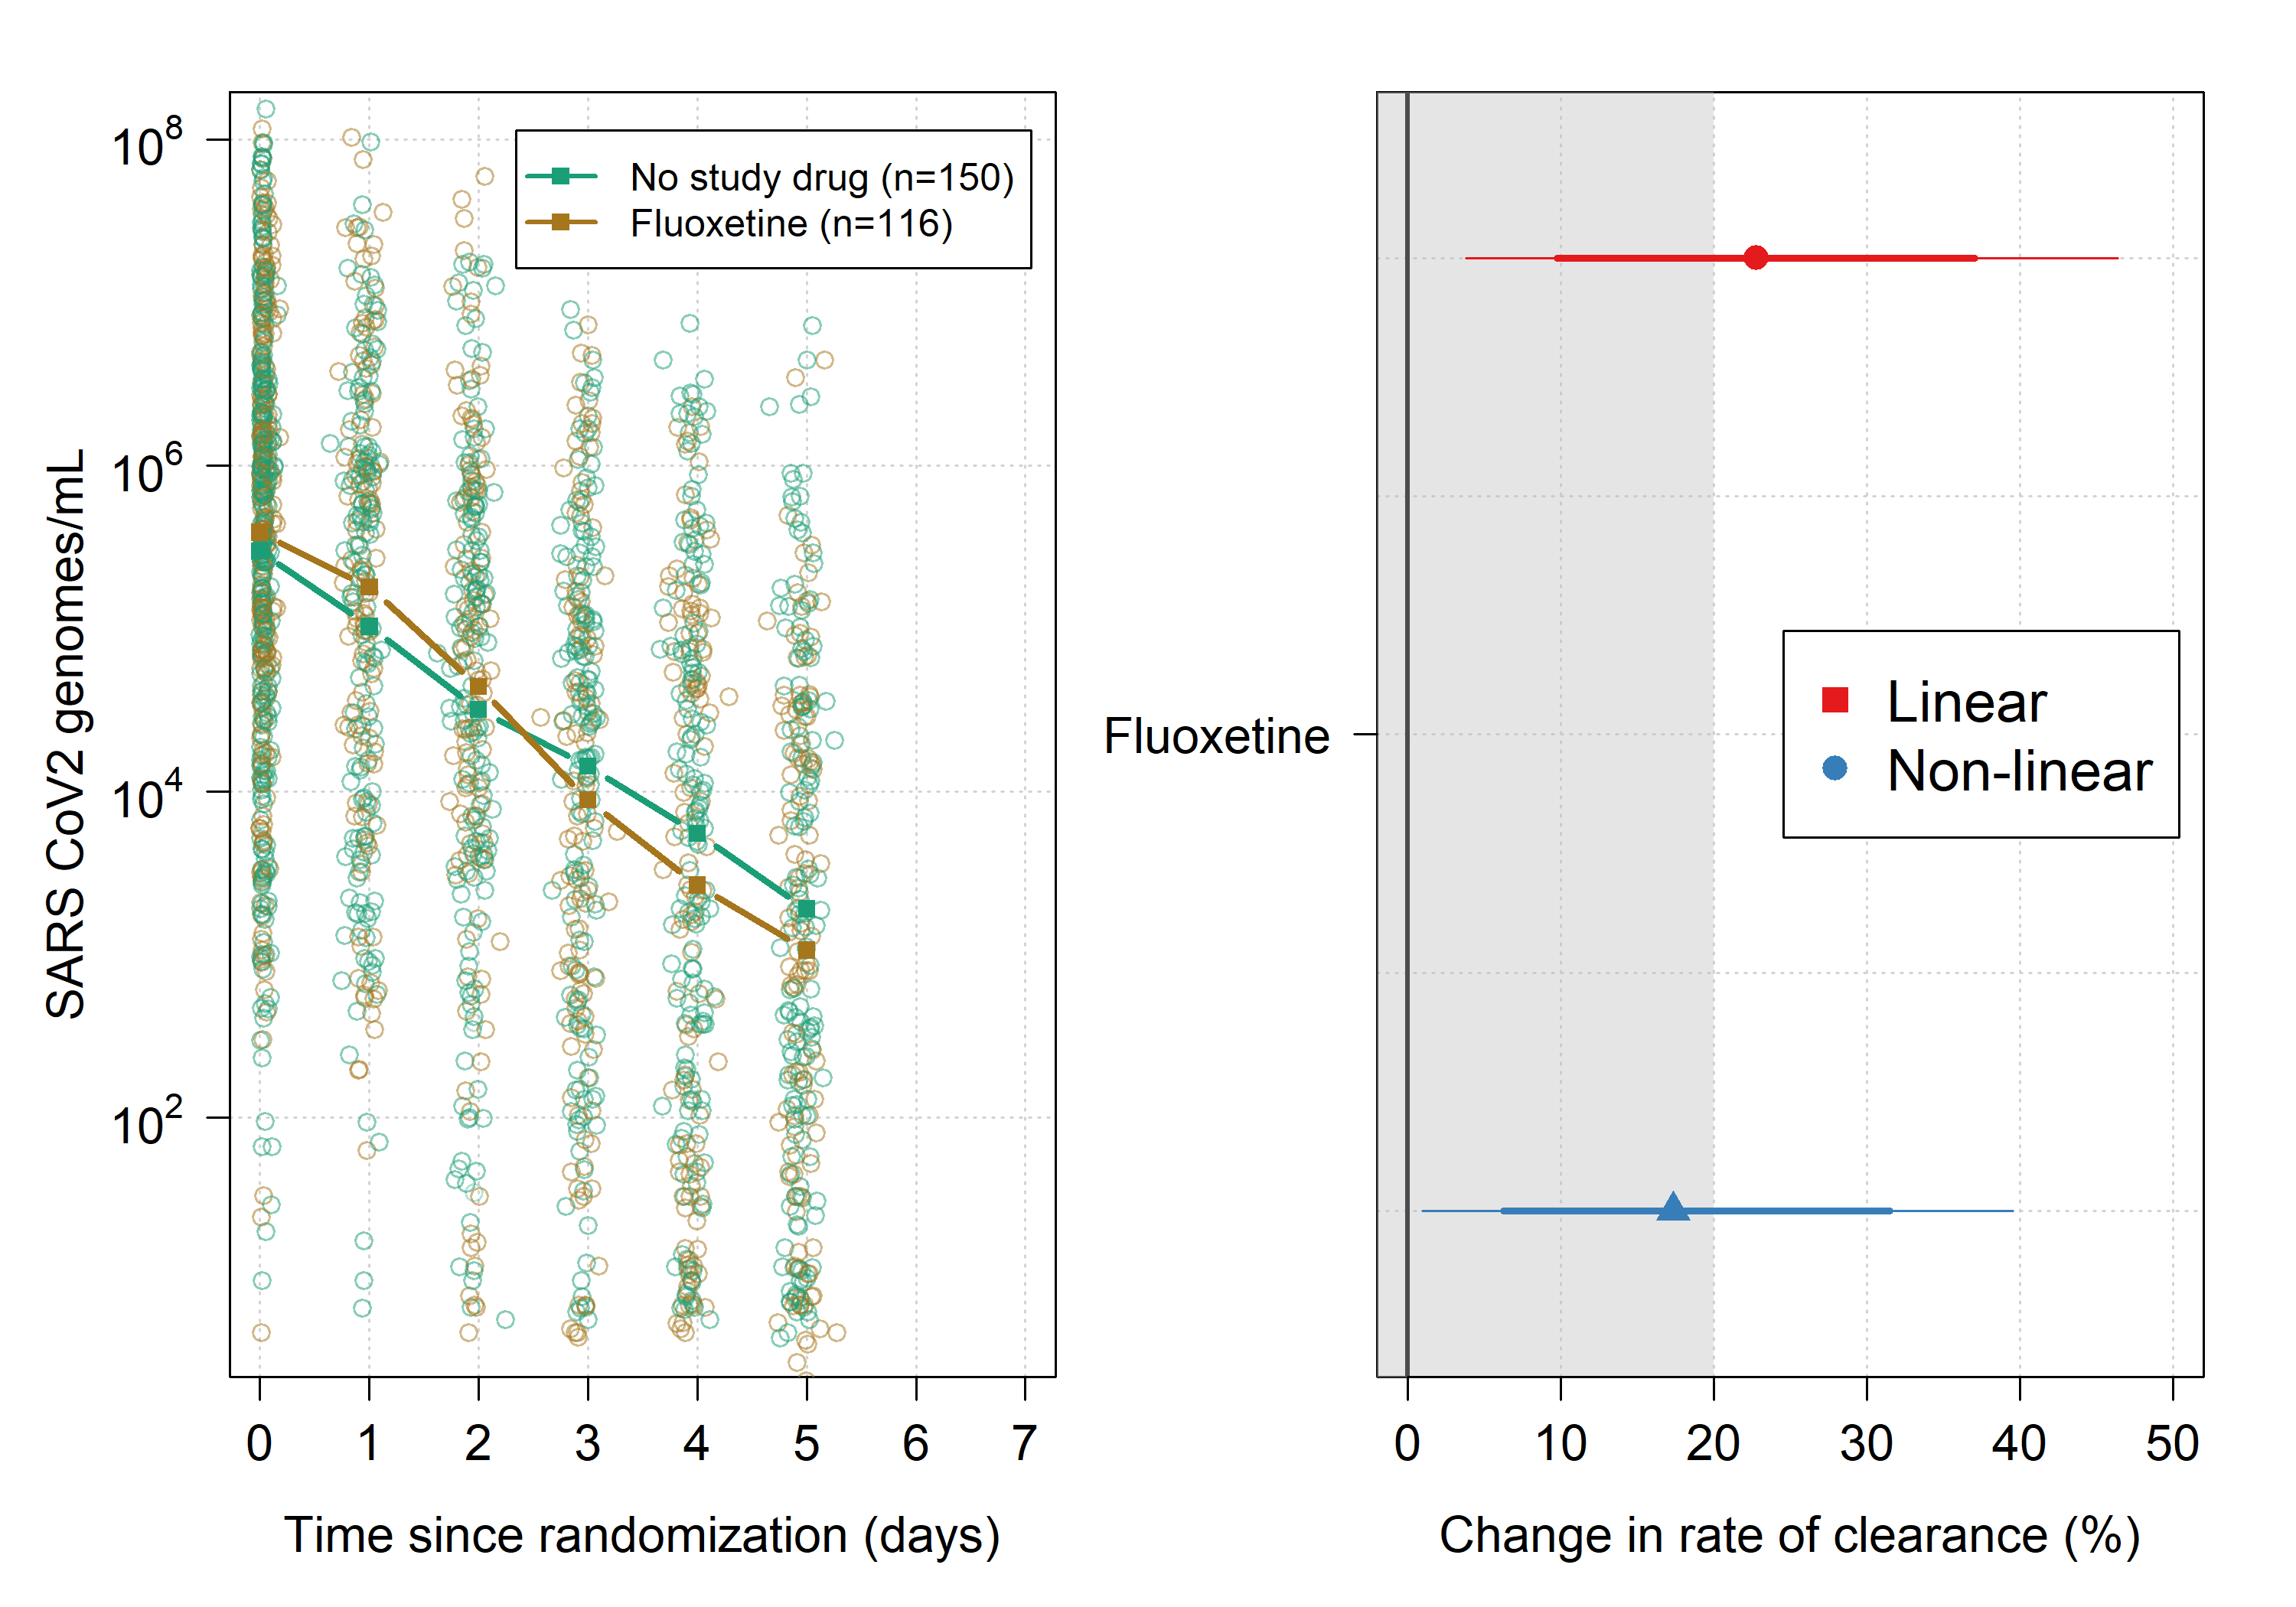
\includegraphics{Fluoxetine_analysis_files/figure-pdf/Figure_main-1.png}

}

\end{figure}

\begin{verbatim}
 2.5%   10%   50%   90% 97.5% 
    4    10    23    37    46 
\end{verbatim}

\begin{verbatim}
Probability that the effect is less than 1.2% is 0.382
\end{verbatim}

\begin{verbatim}
 2.5%   10%   50%   90% 97.5% 
    1     6    17    31    40 
\end{verbatim}

\begin{verbatim}
Probability that the effect is less than 1.2% is 0.592
\end{verbatim}

\begin{figure}[H]

{\centering 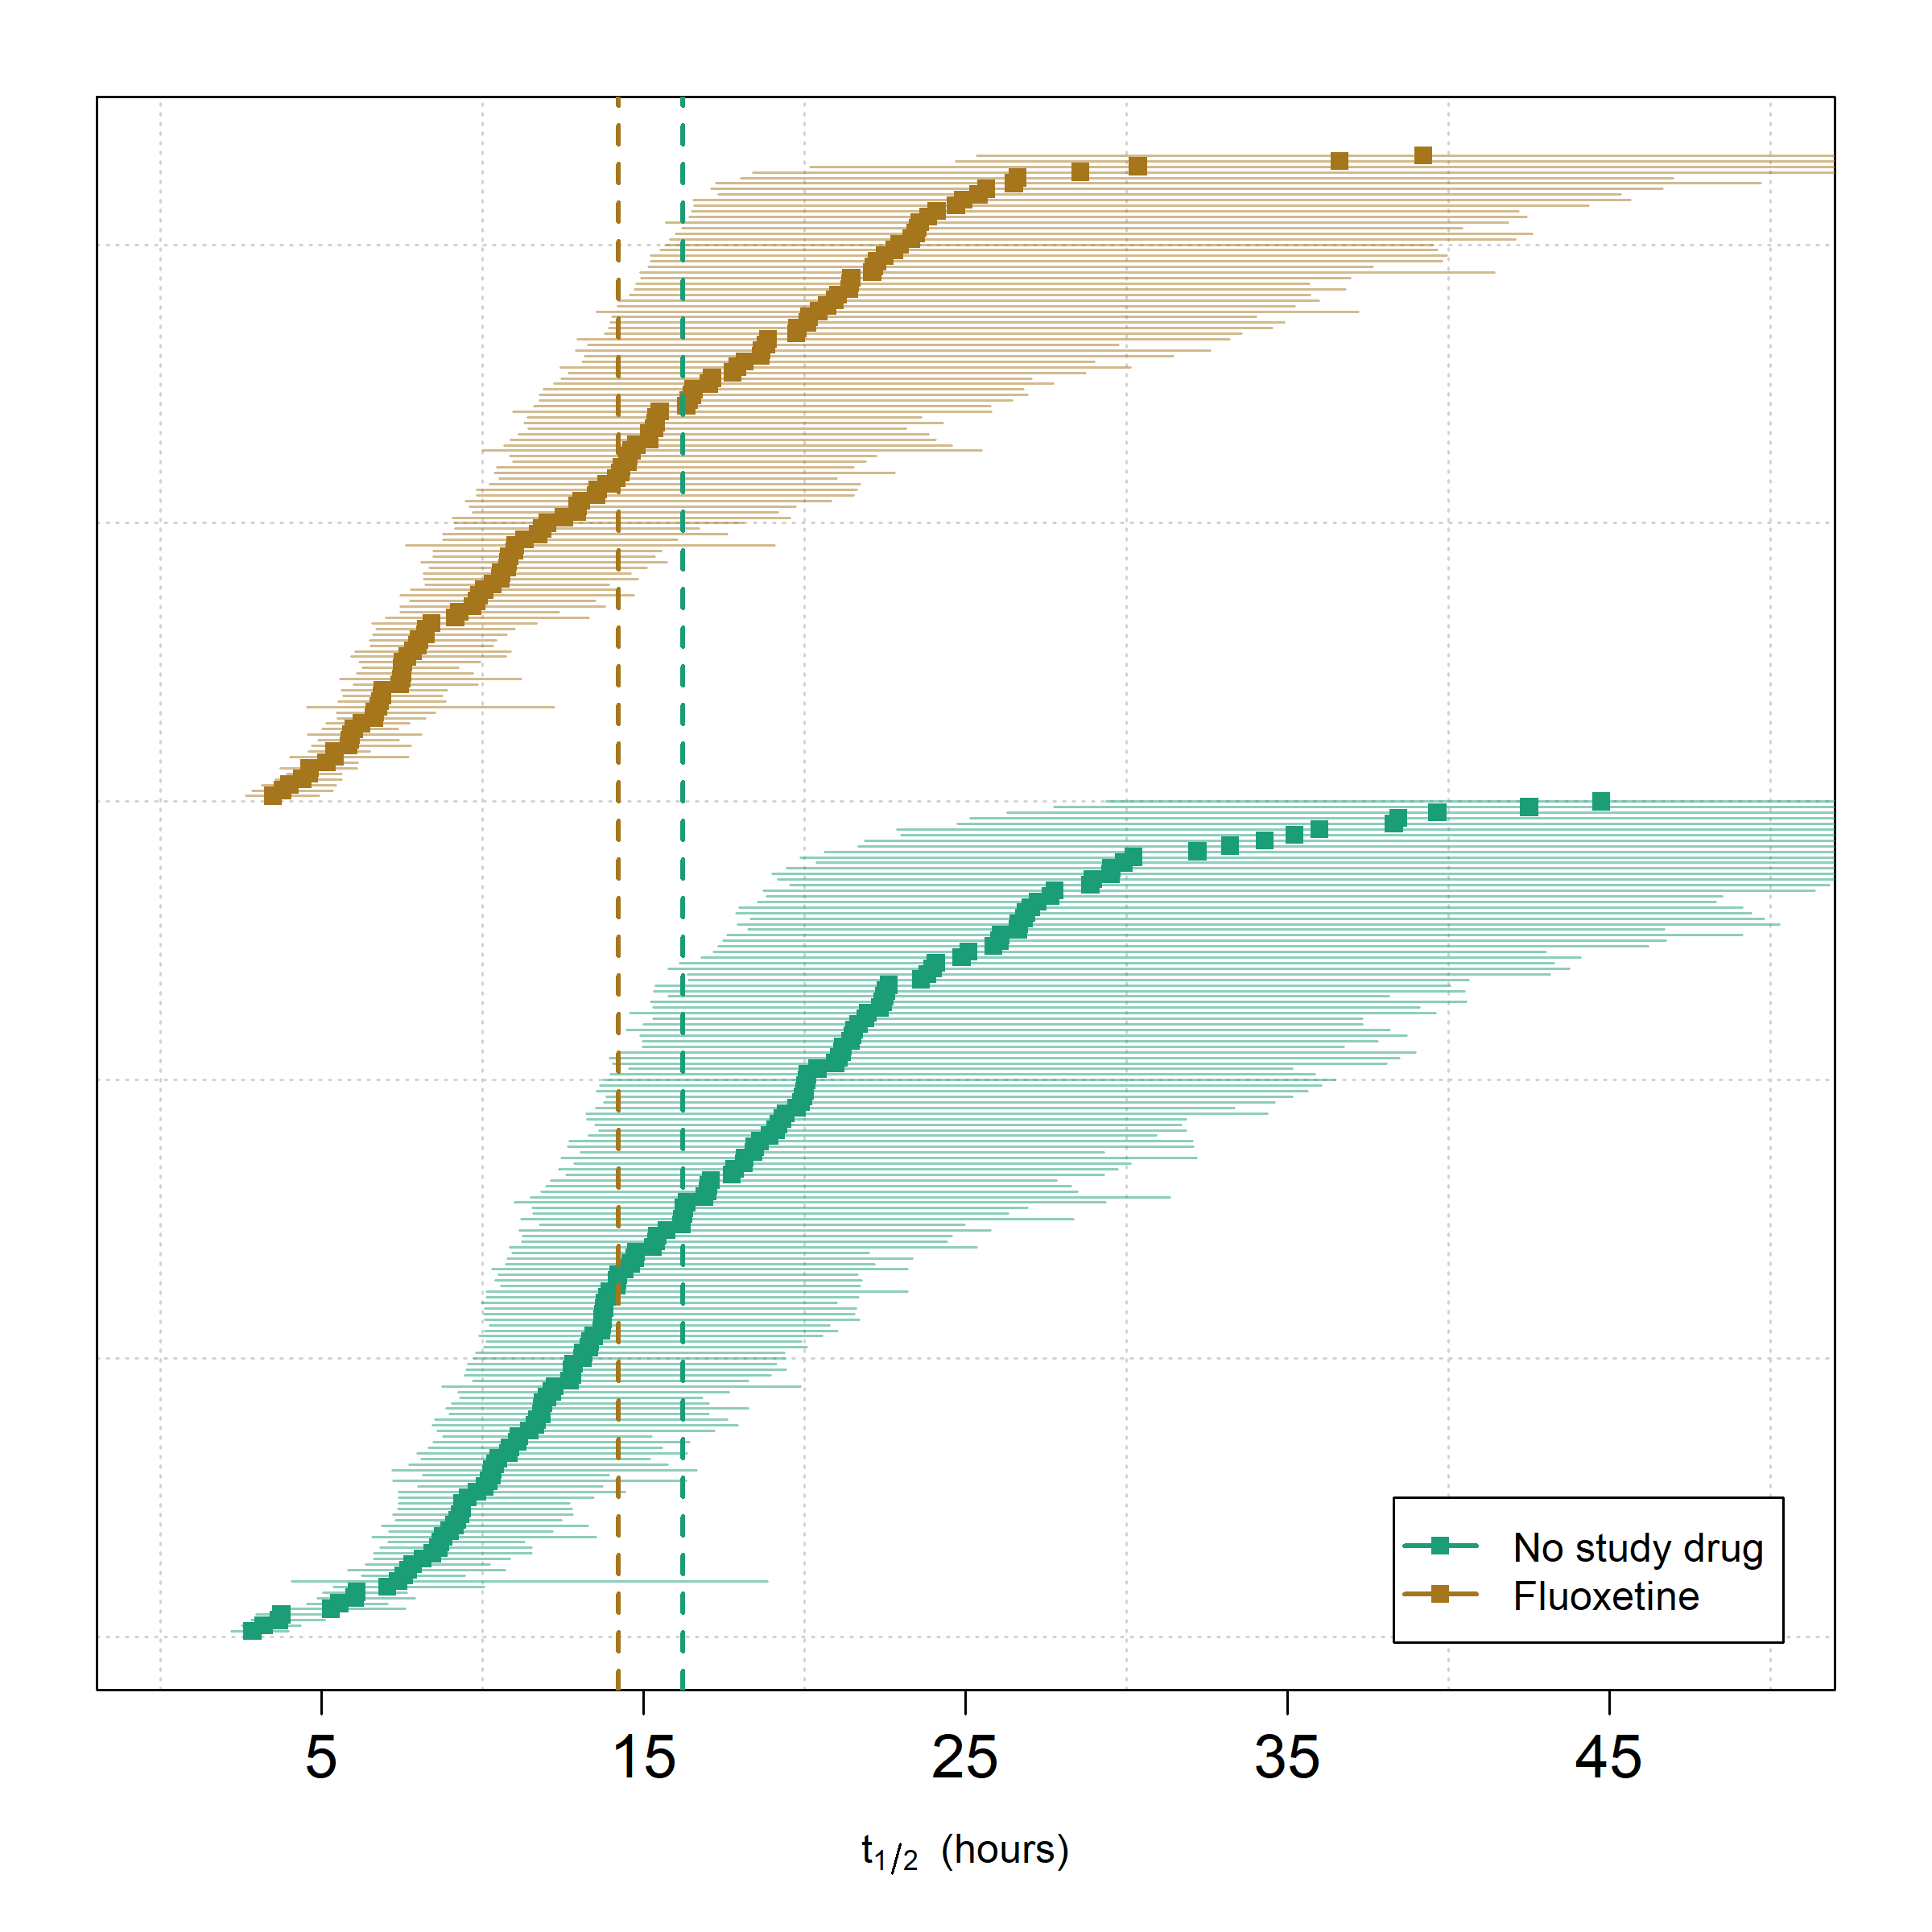
\includegraphics{Fluoxetine_analysis_files/figure-pdf/slopes_plot-1.png}

}

\end{figure}

\begin{verbatim}
In No study drug the median clearance half life was 16.2 (range 2.8 to 44.7)
In Fluoxetine the median clearance half life was 14.2 (range 3.5 to 39.2)
\end{verbatim}

\begin{verbatim}
The following `from` values were not present in `x`: Age_scaled, Antibody_test, Symptom_onset, N_dose
The following `from` values were not present in `x`: Age_scaled, Antibody_test, Symptom_onset, N_dose
\end{verbatim}

\begin{figure}[H]

{\centering 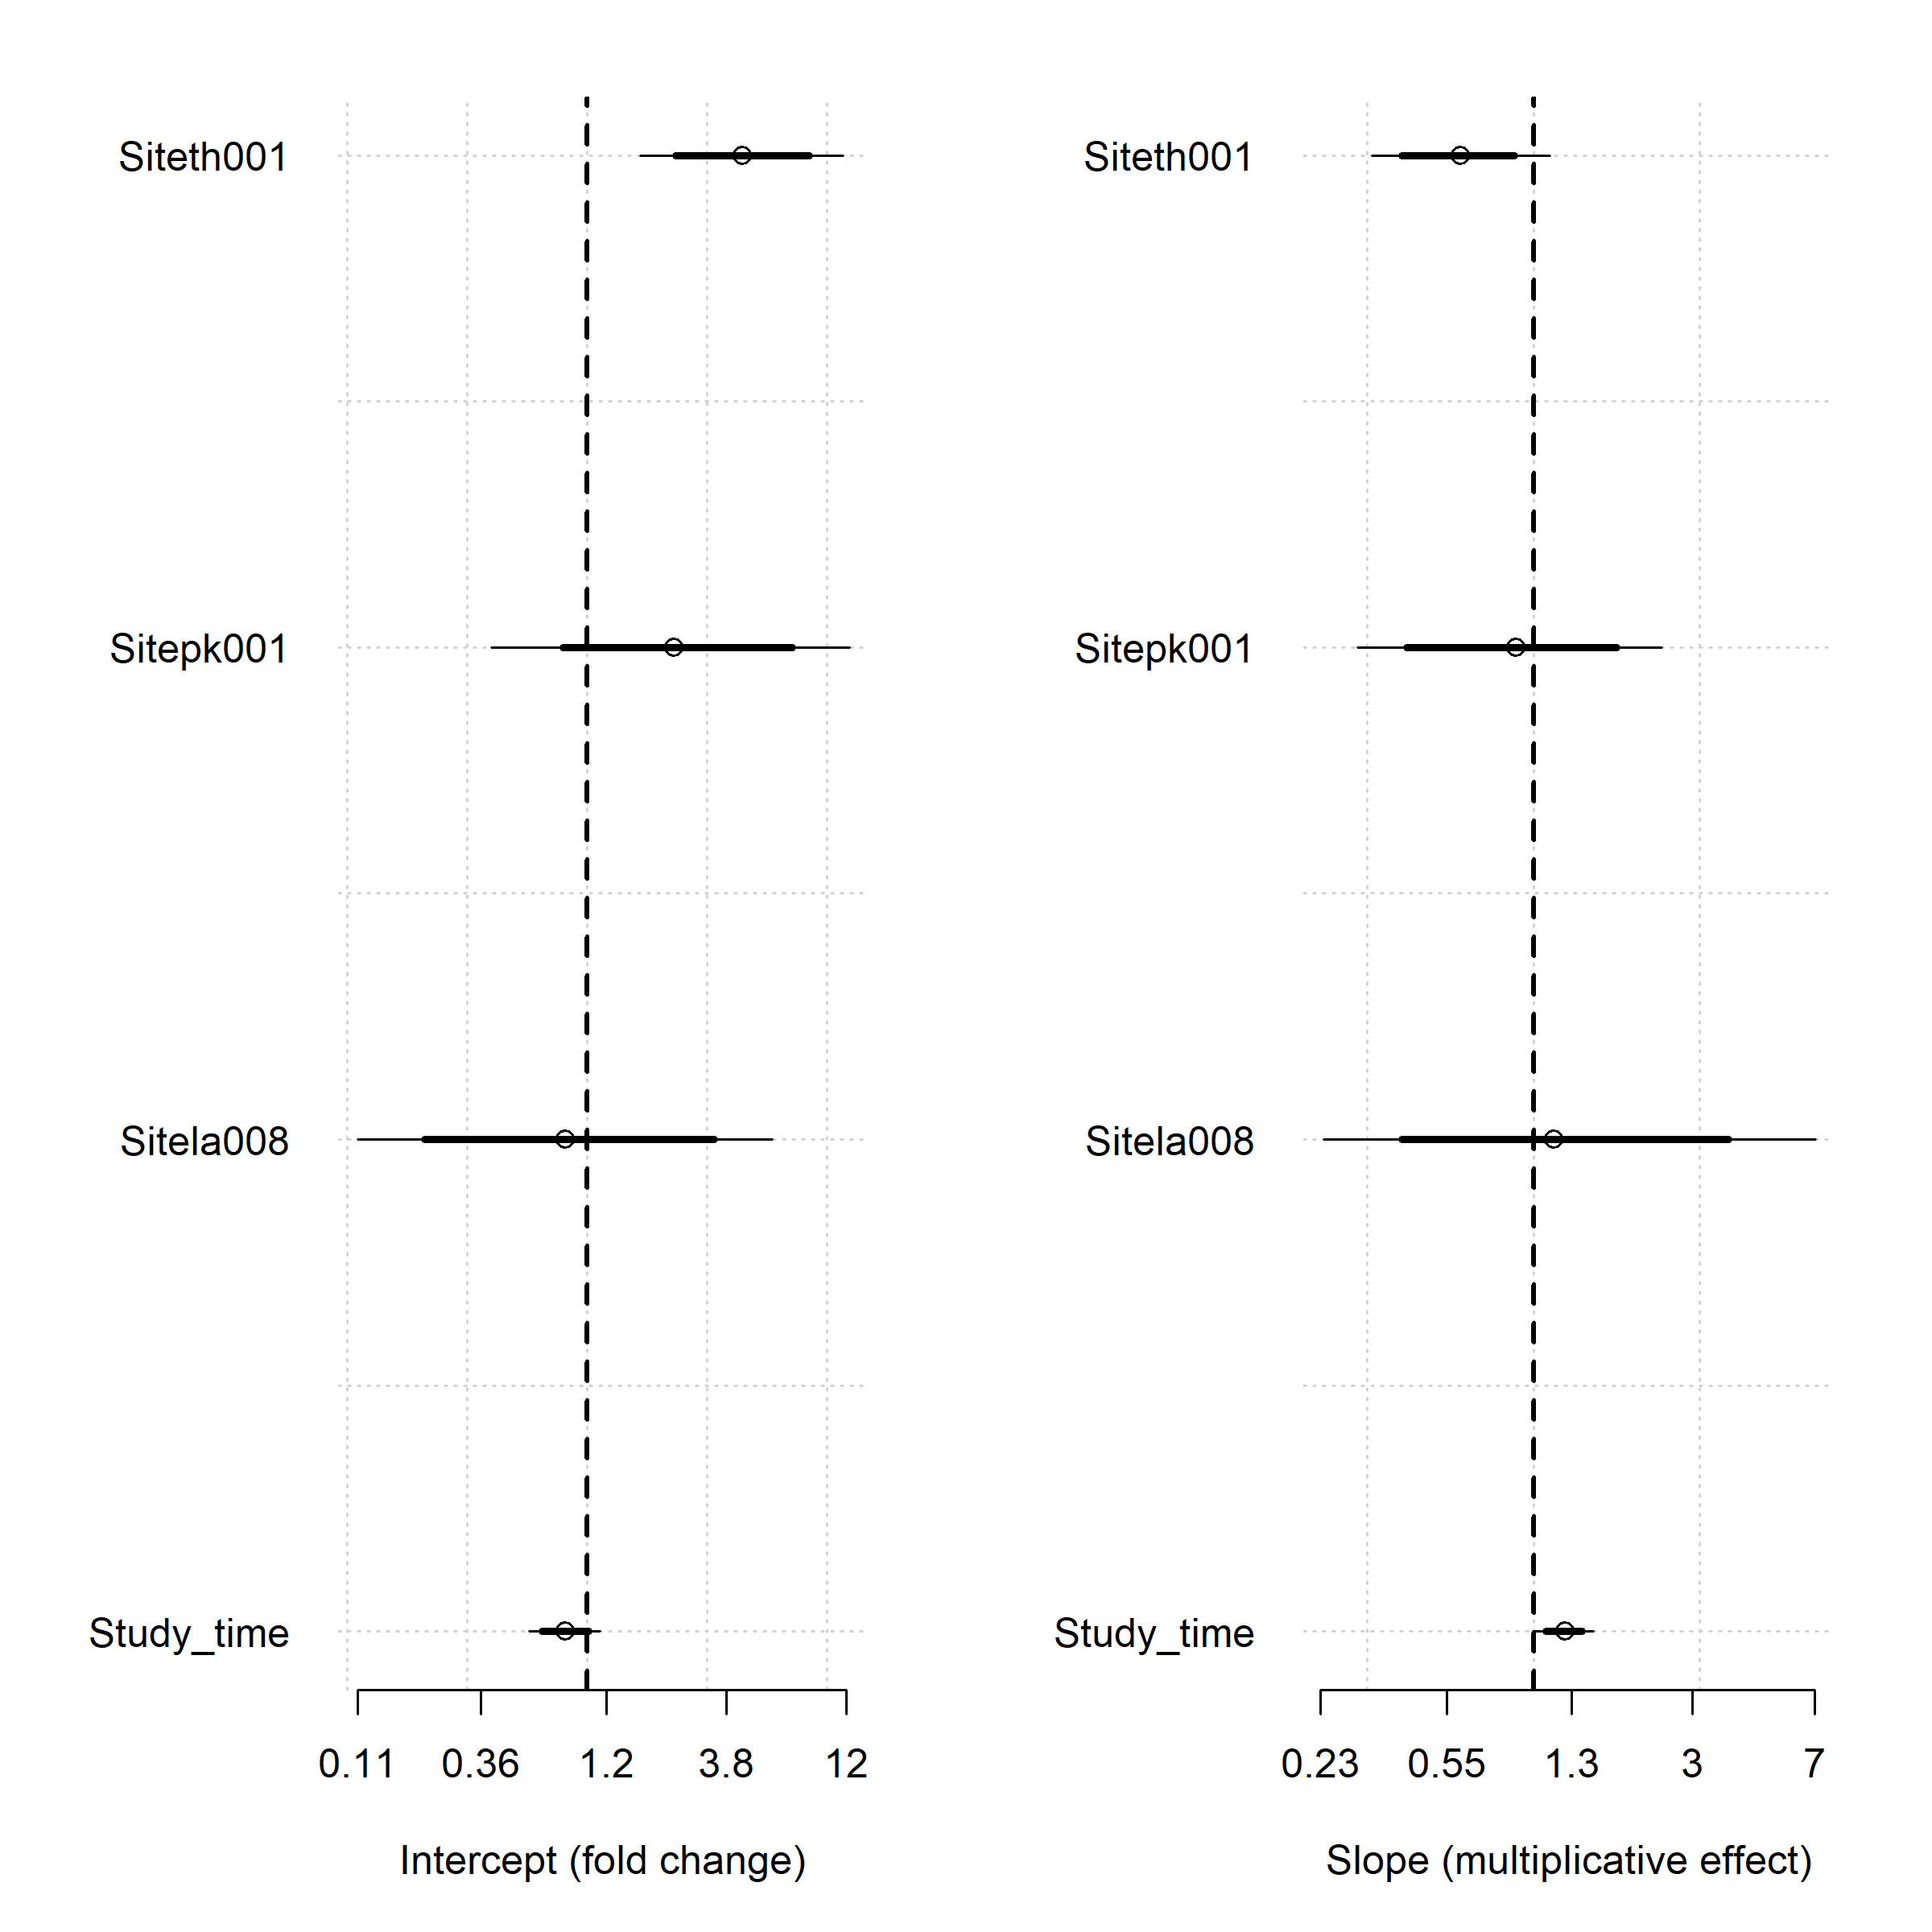
\includegraphics{Fluoxetine_analysis_files/figure-pdf/coef_plot-1.png}

}

\end{figure}

\hypertarget{individual-patient-data}{%
\subsection{Individual patient data}\label{individual-patient-data}}

\begin{figure}[H]

{\centering 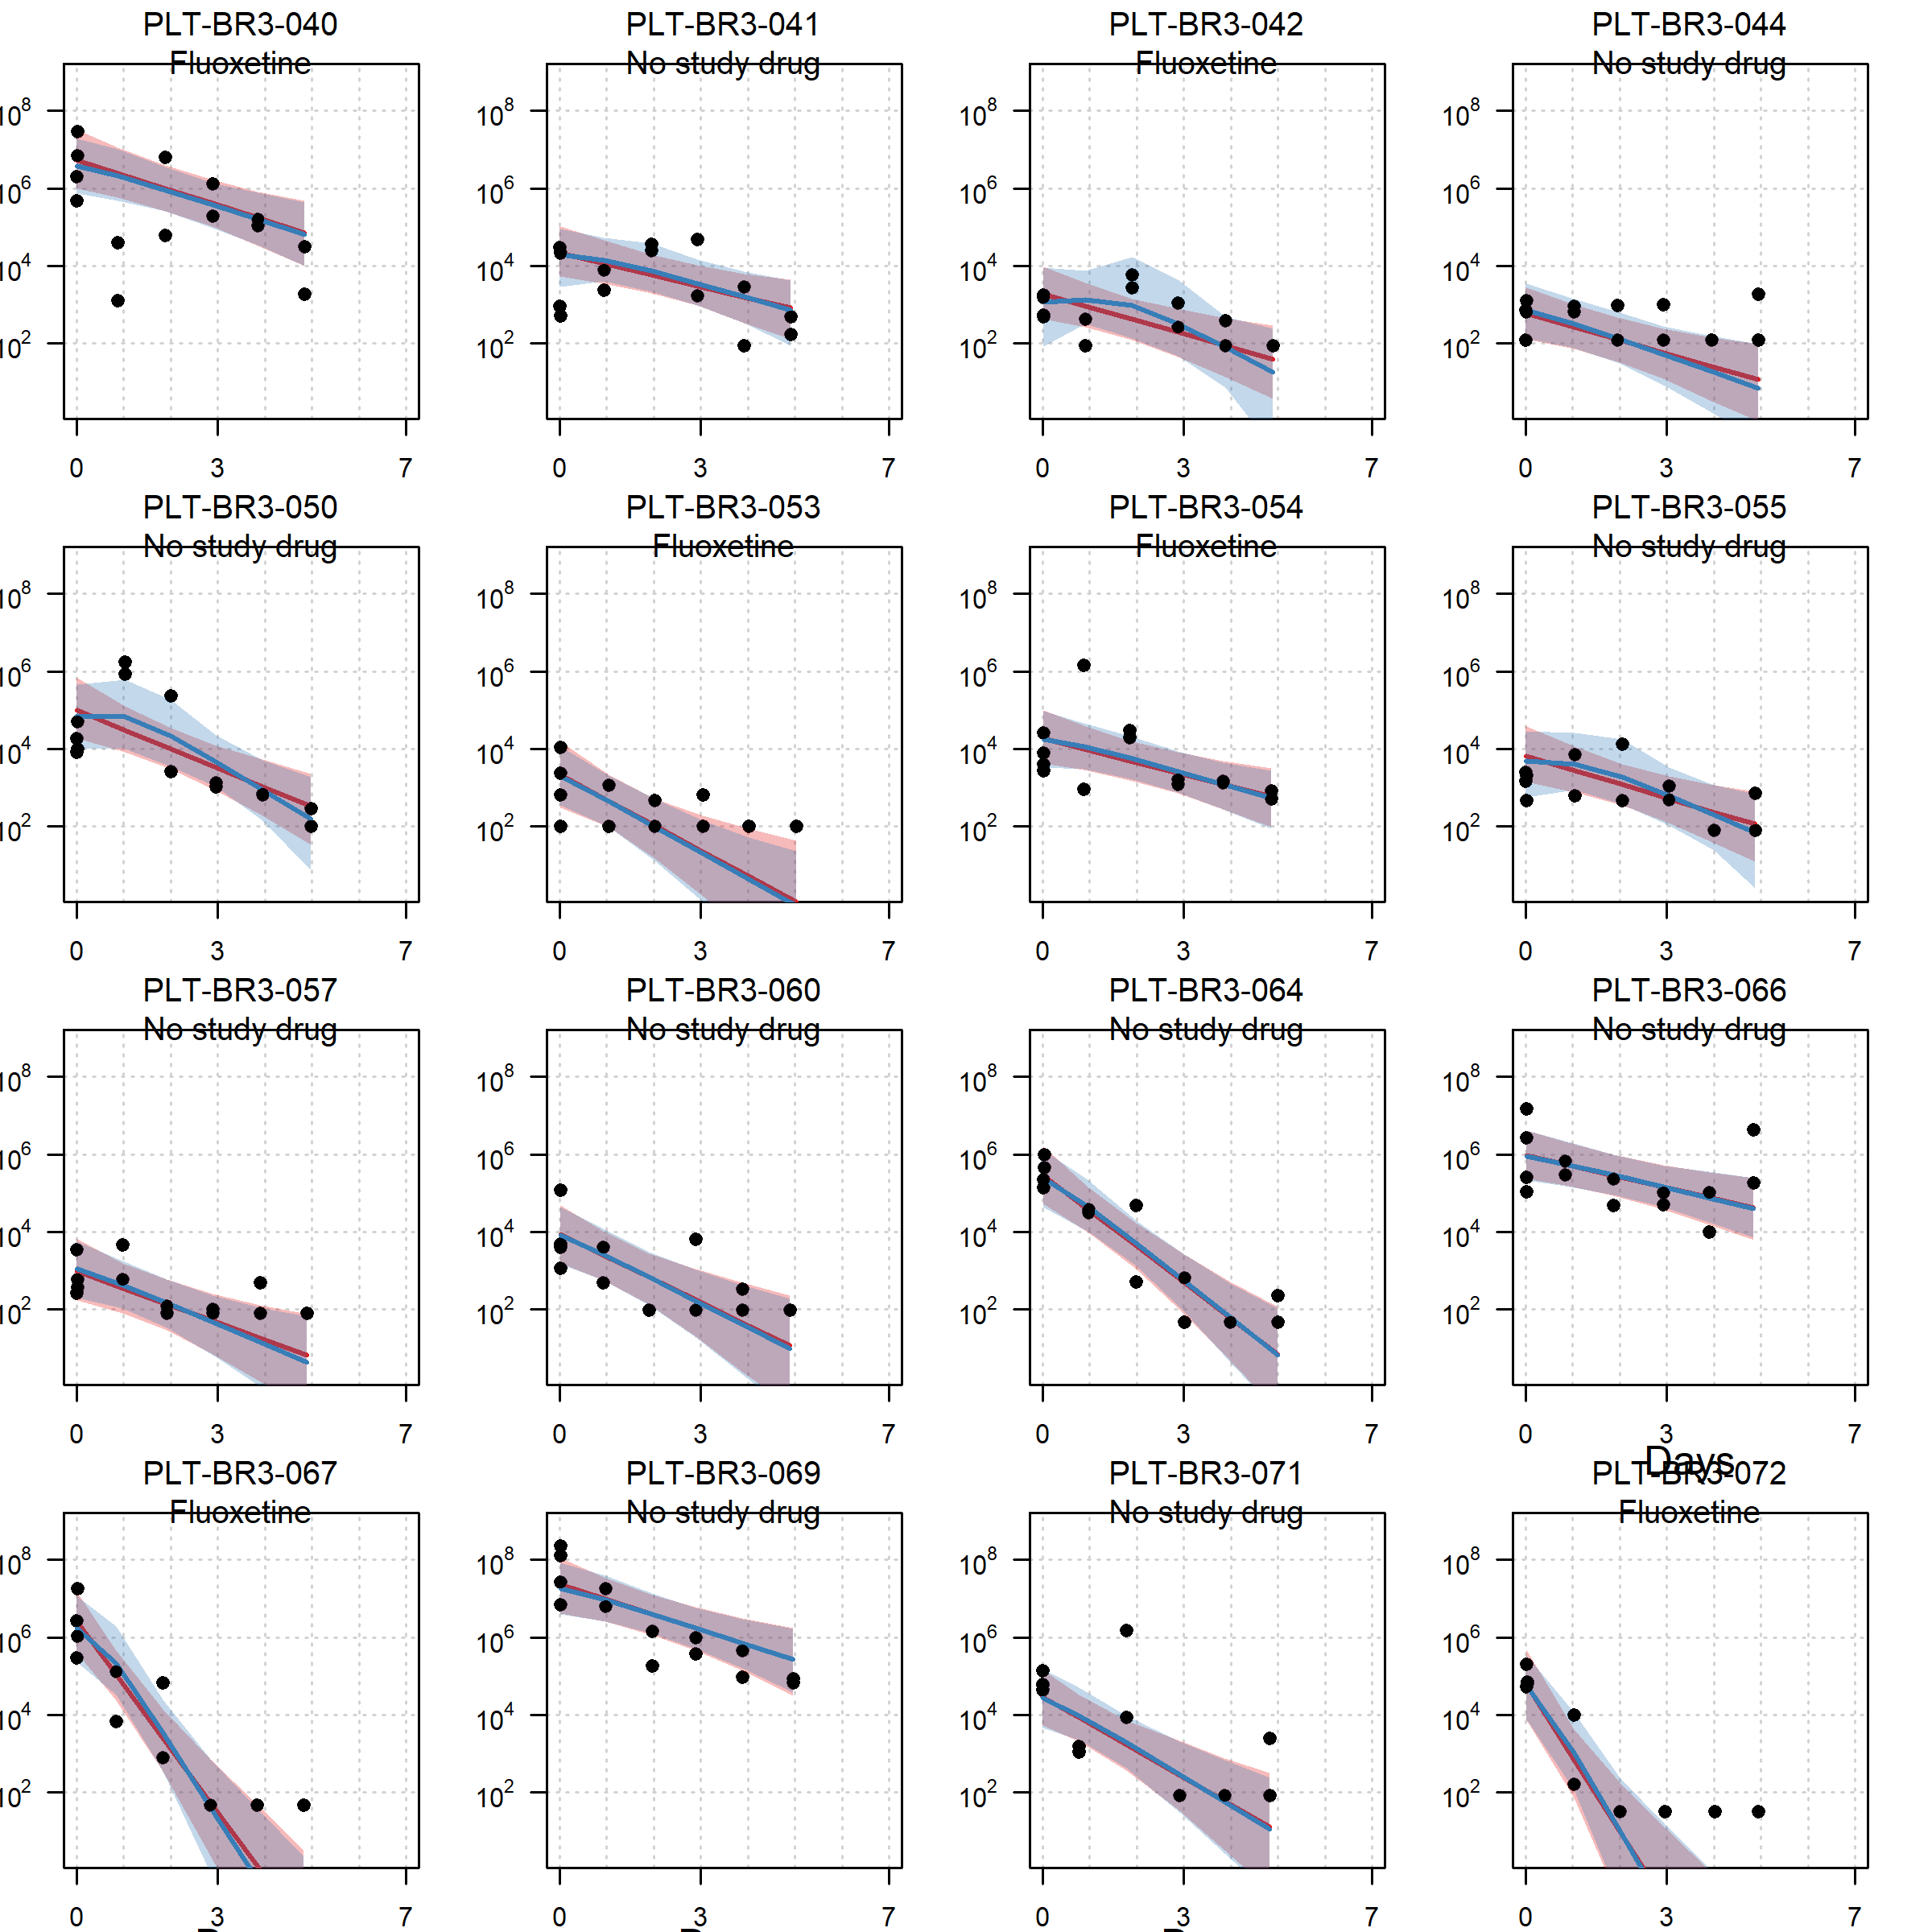
\includegraphics{Fluoxetine_analysis_files/figure-pdf/individ_data-1.png}

}

\end{figure}

\begin{figure}[H]

{\centering 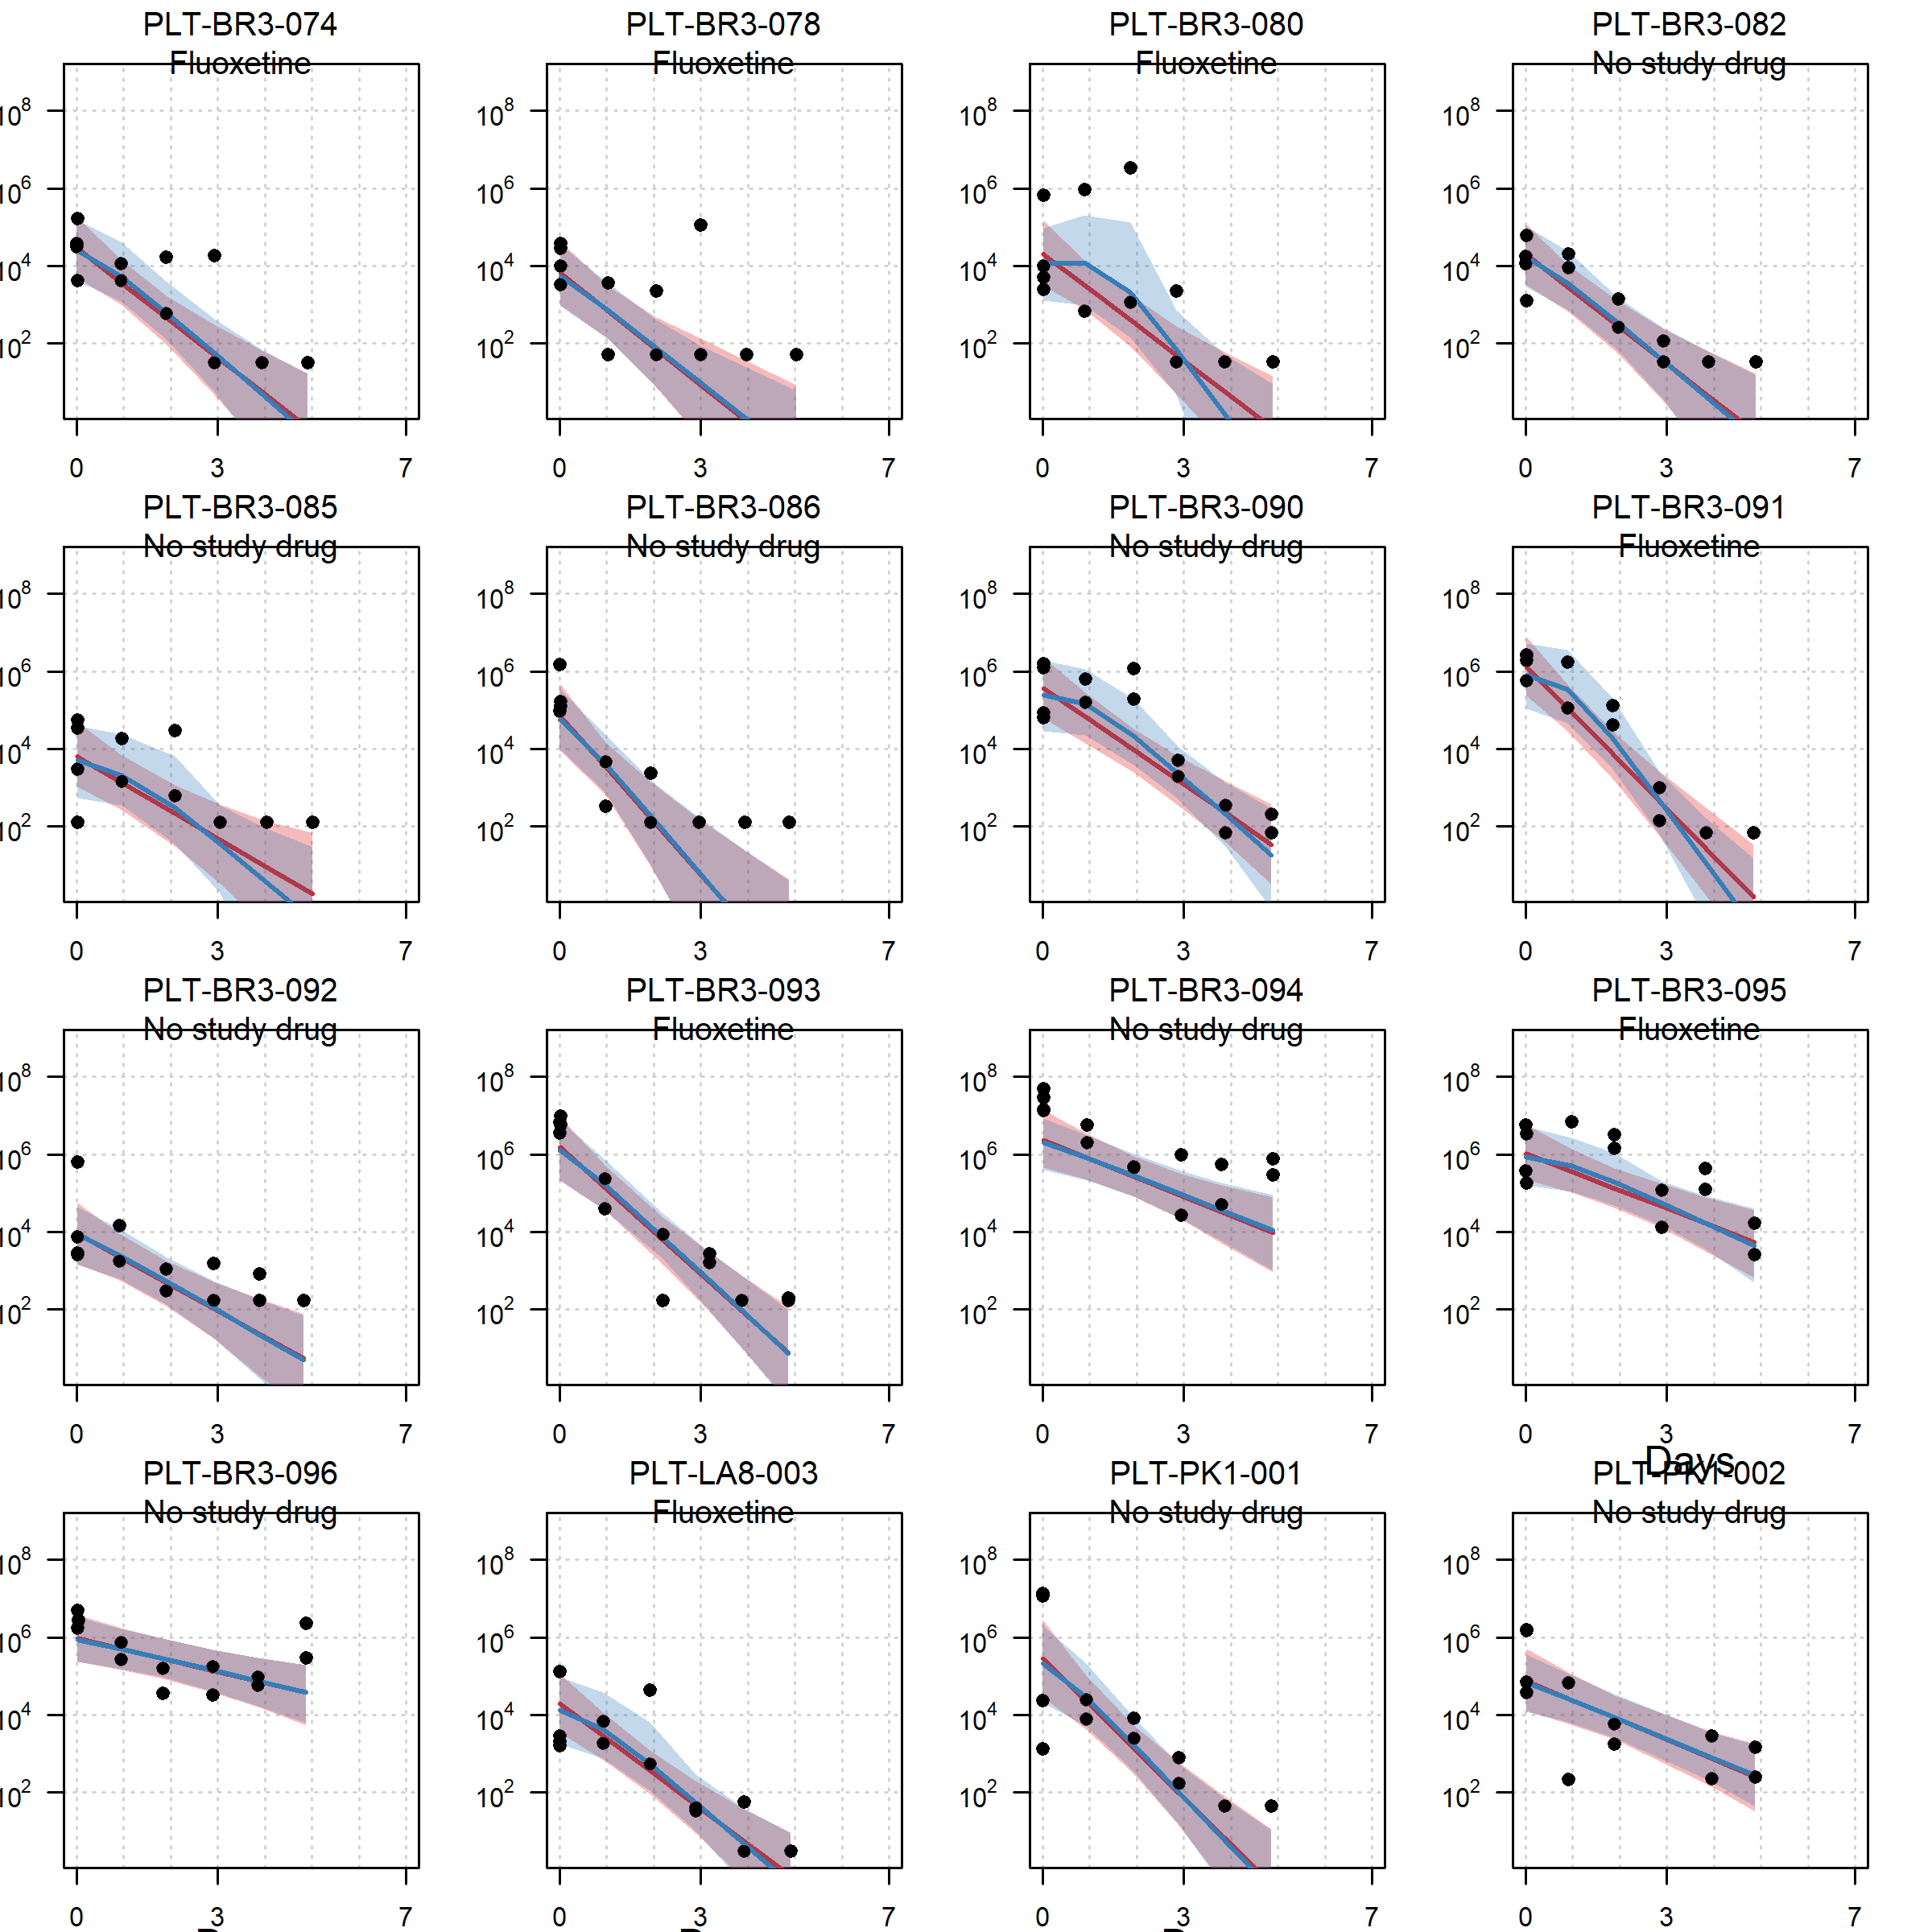
\includegraphics{Fluoxetine_analysis_files/figure-pdf/individ_data-2.png}

}

\end{figure}

\begin{figure}[H]

{\centering 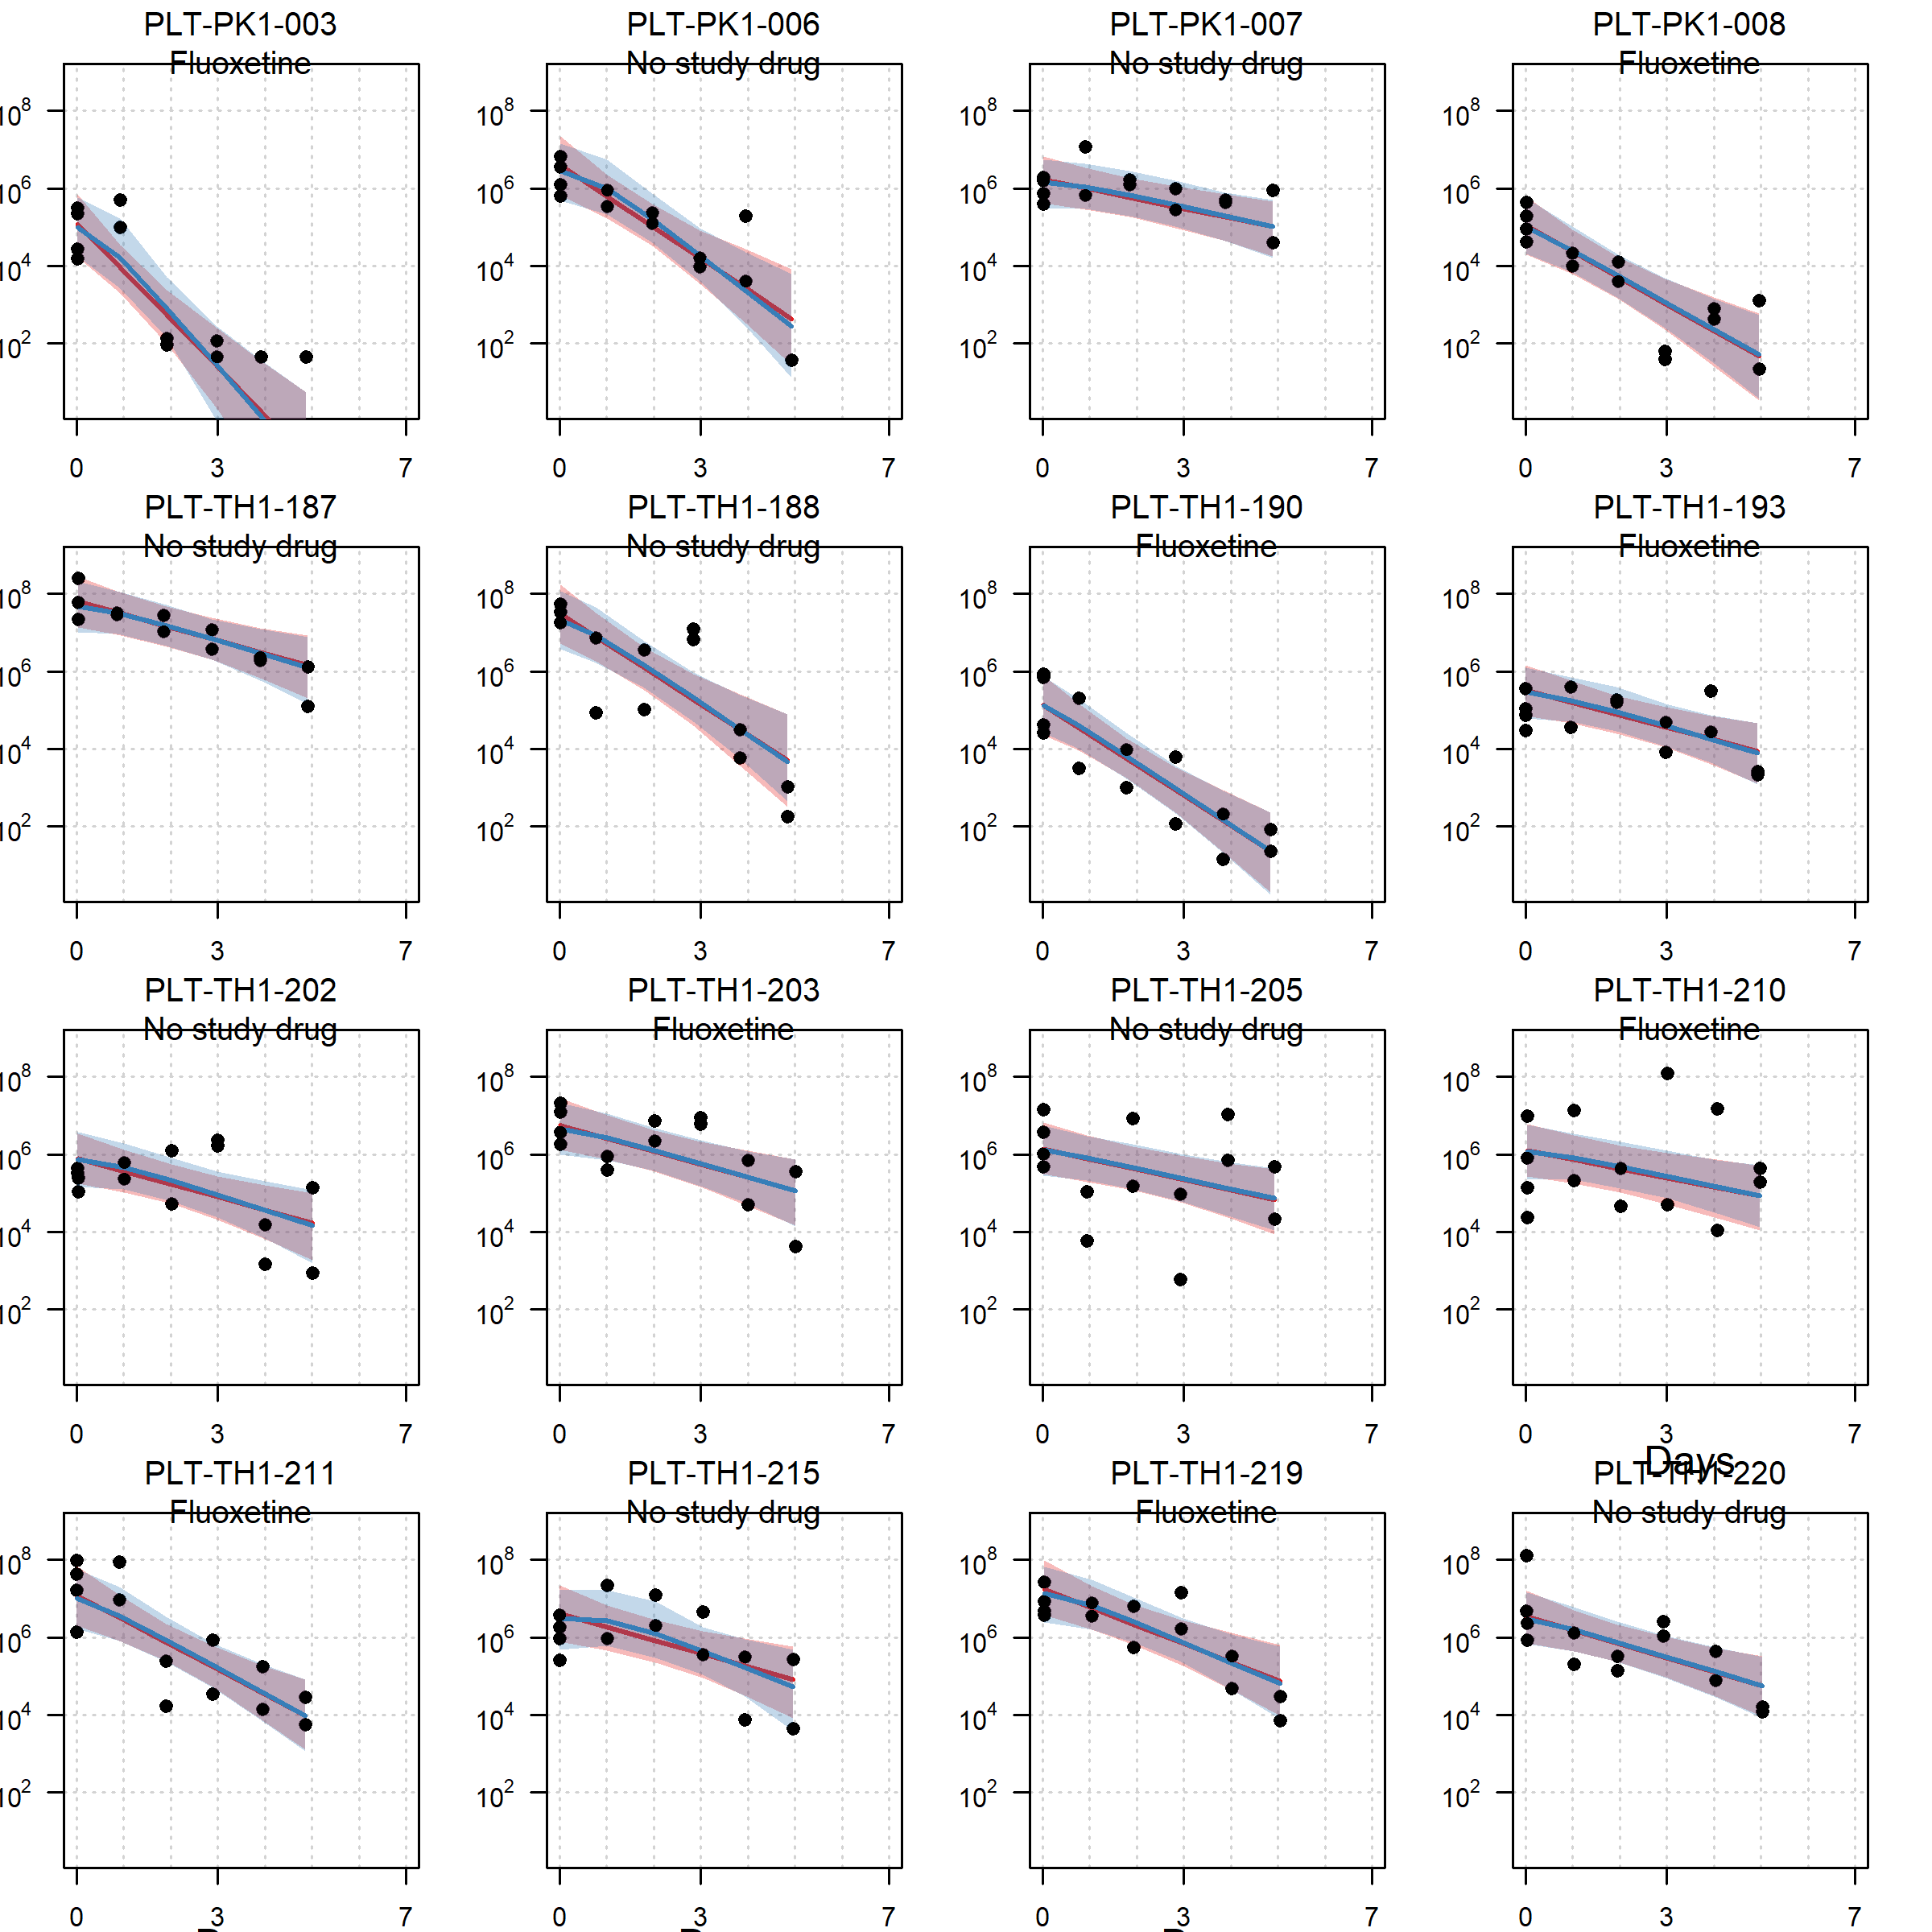
\includegraphics{Fluoxetine_analysis_files/figure-pdf/individ_data-3.png}

}

\end{figure}

\begin{figure}[H]

{\centering 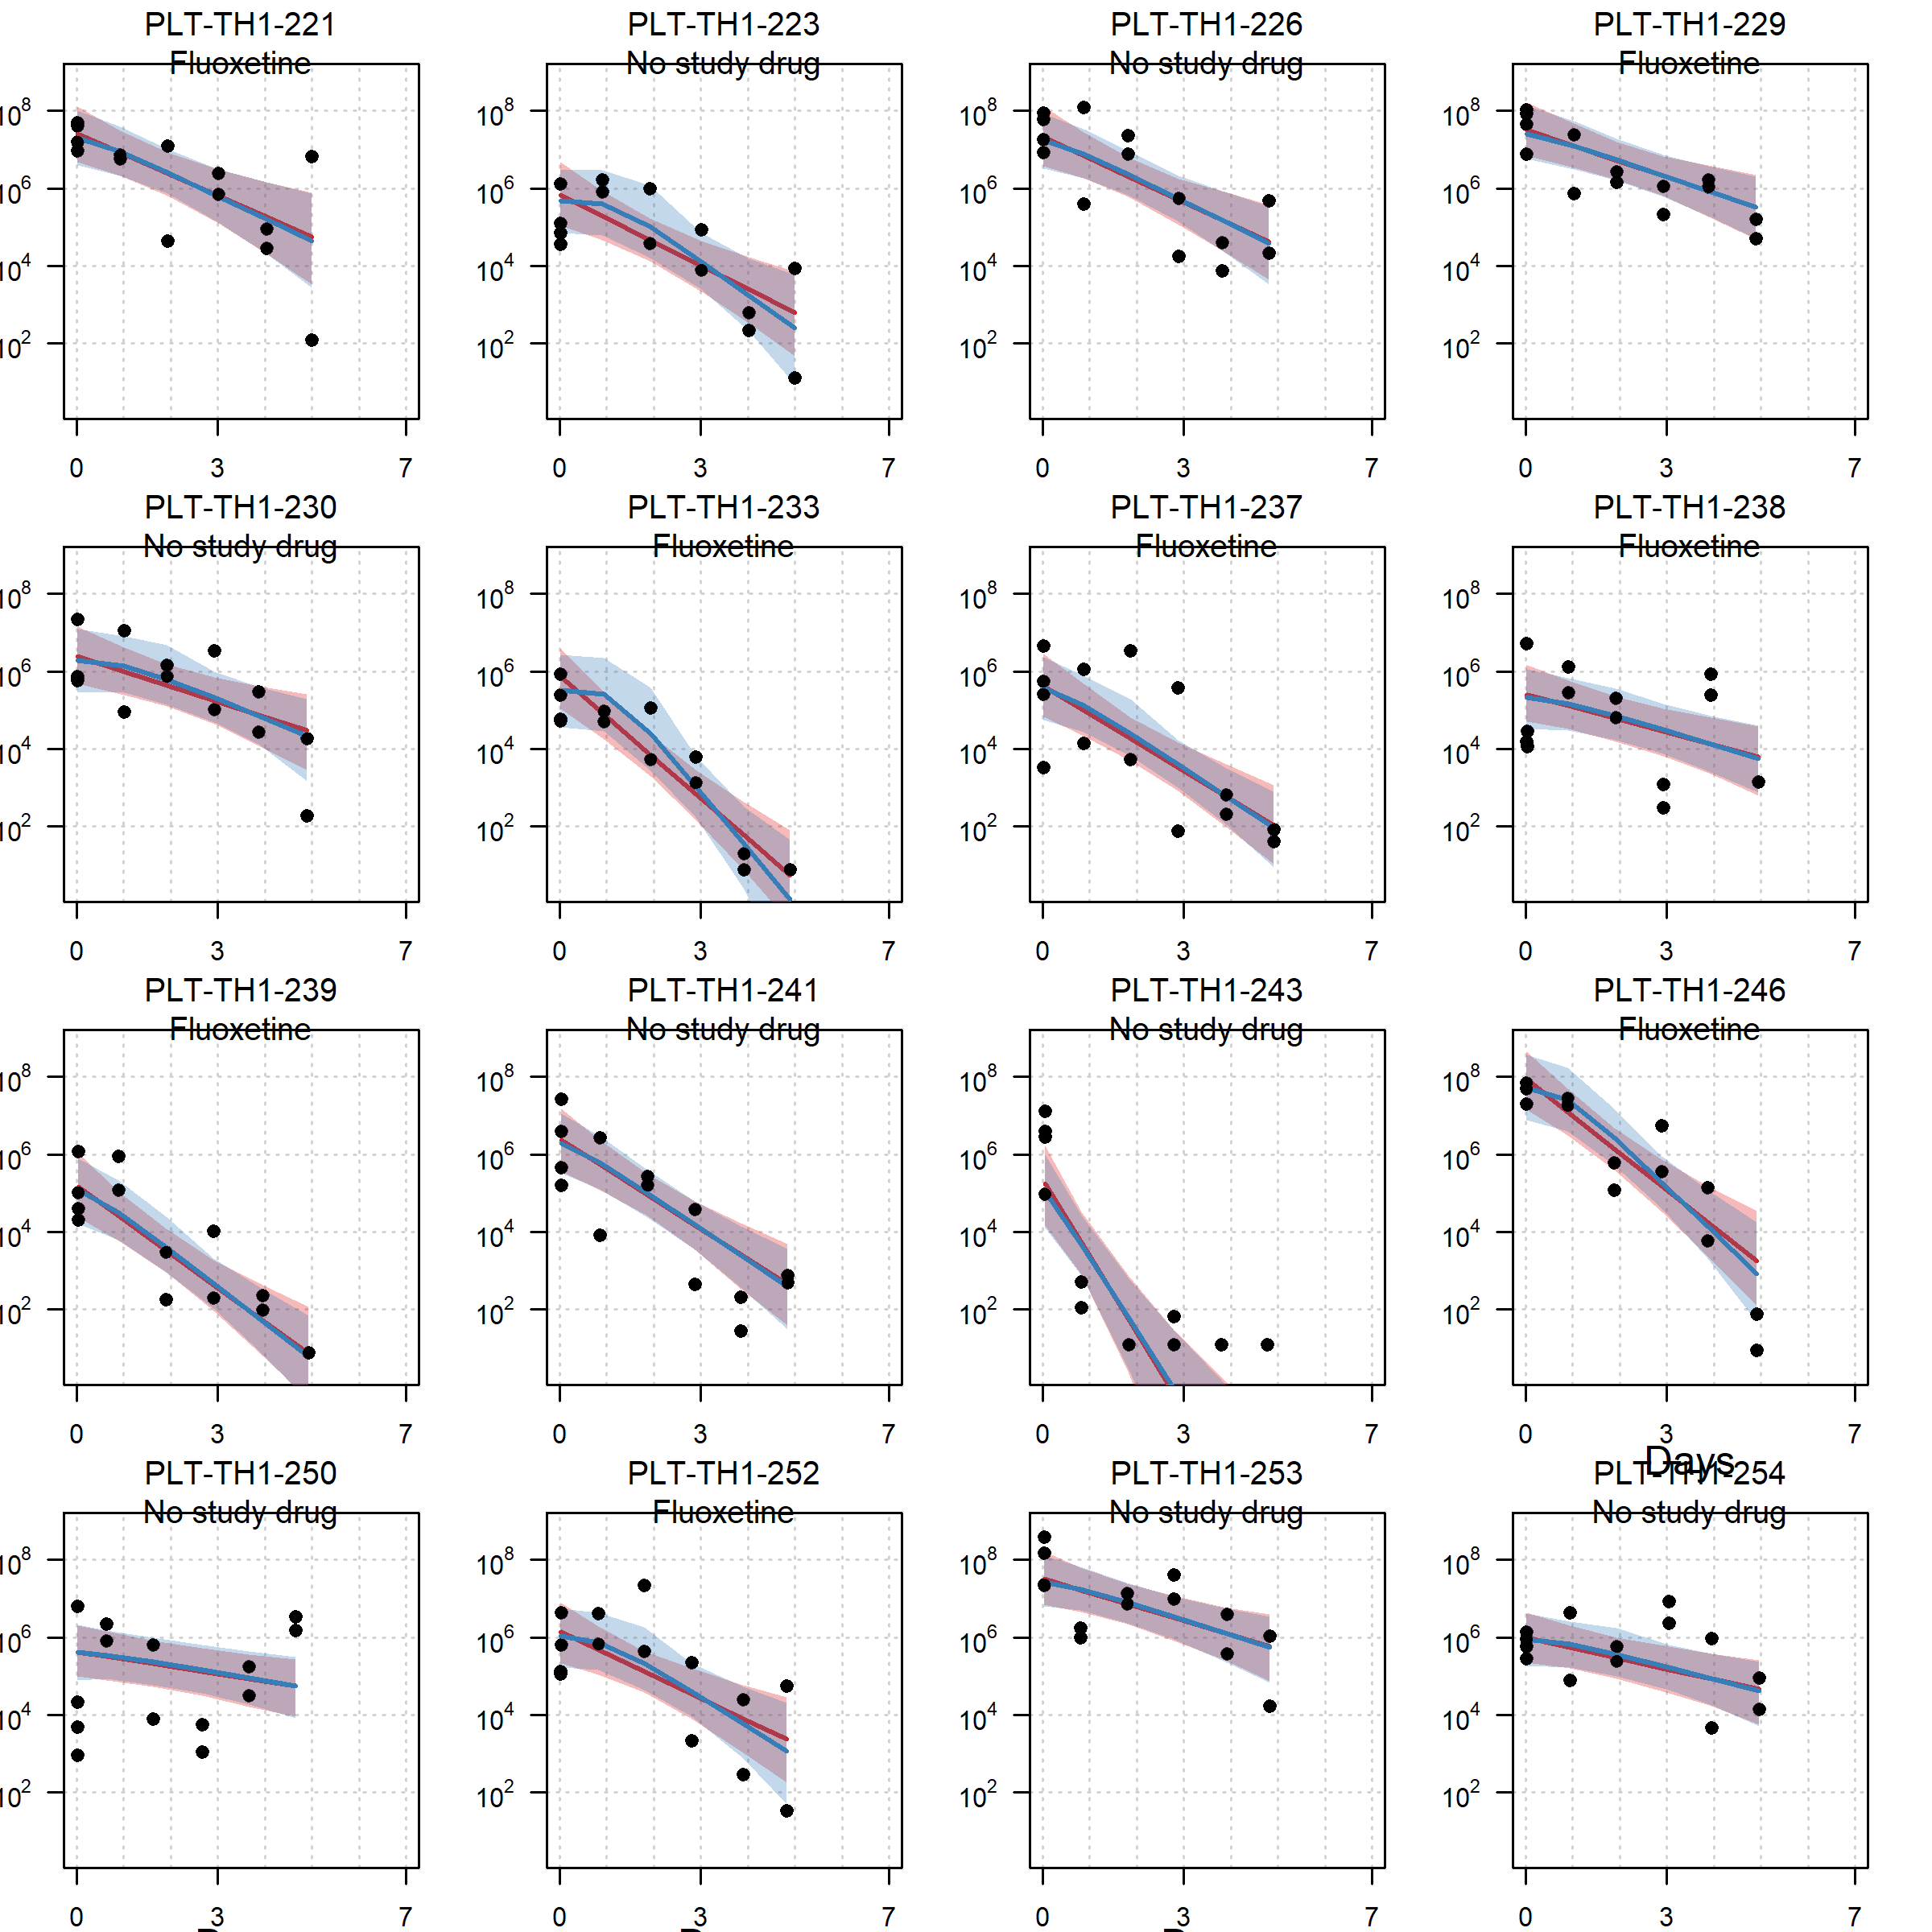
\includegraphics{Fluoxetine_analysis_files/figure-pdf/individ_data-4.png}

}

\end{figure}

\begin{figure}[H]

{\centering 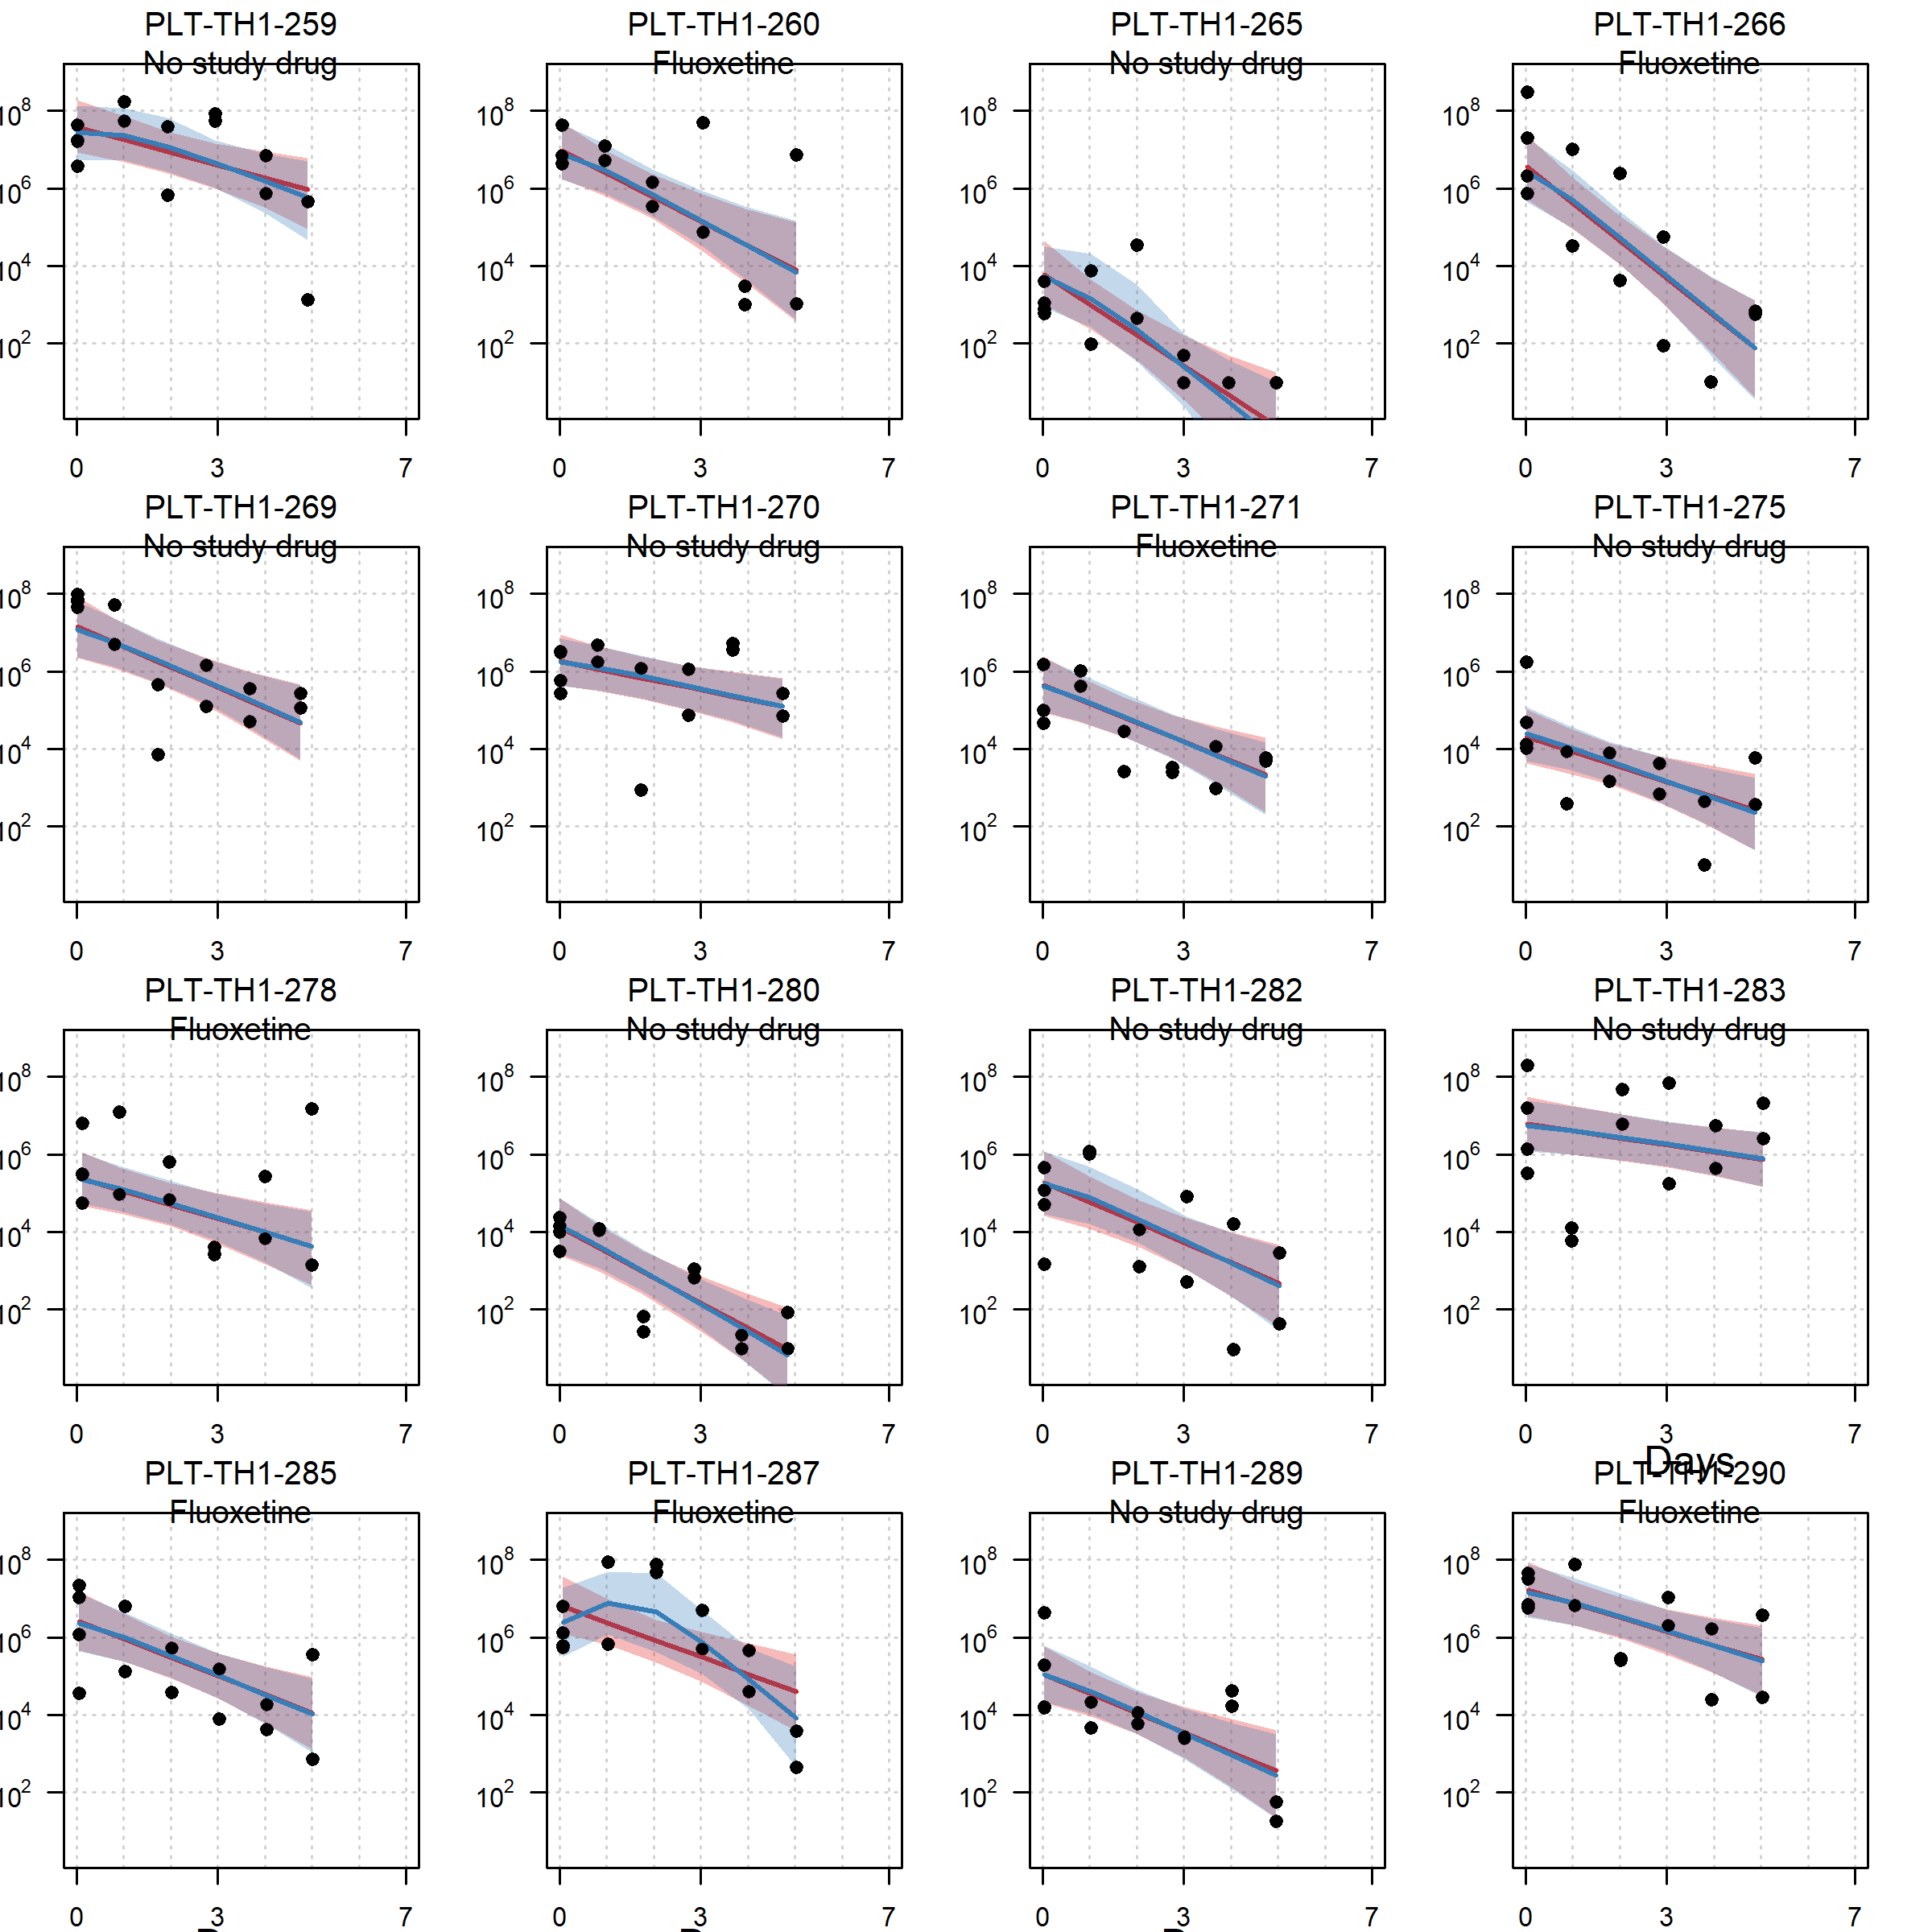
\includegraphics{Fluoxetine_analysis_files/figure-pdf/individ_data-5.png}

}

\end{figure}

\begin{figure}[H]

{\centering 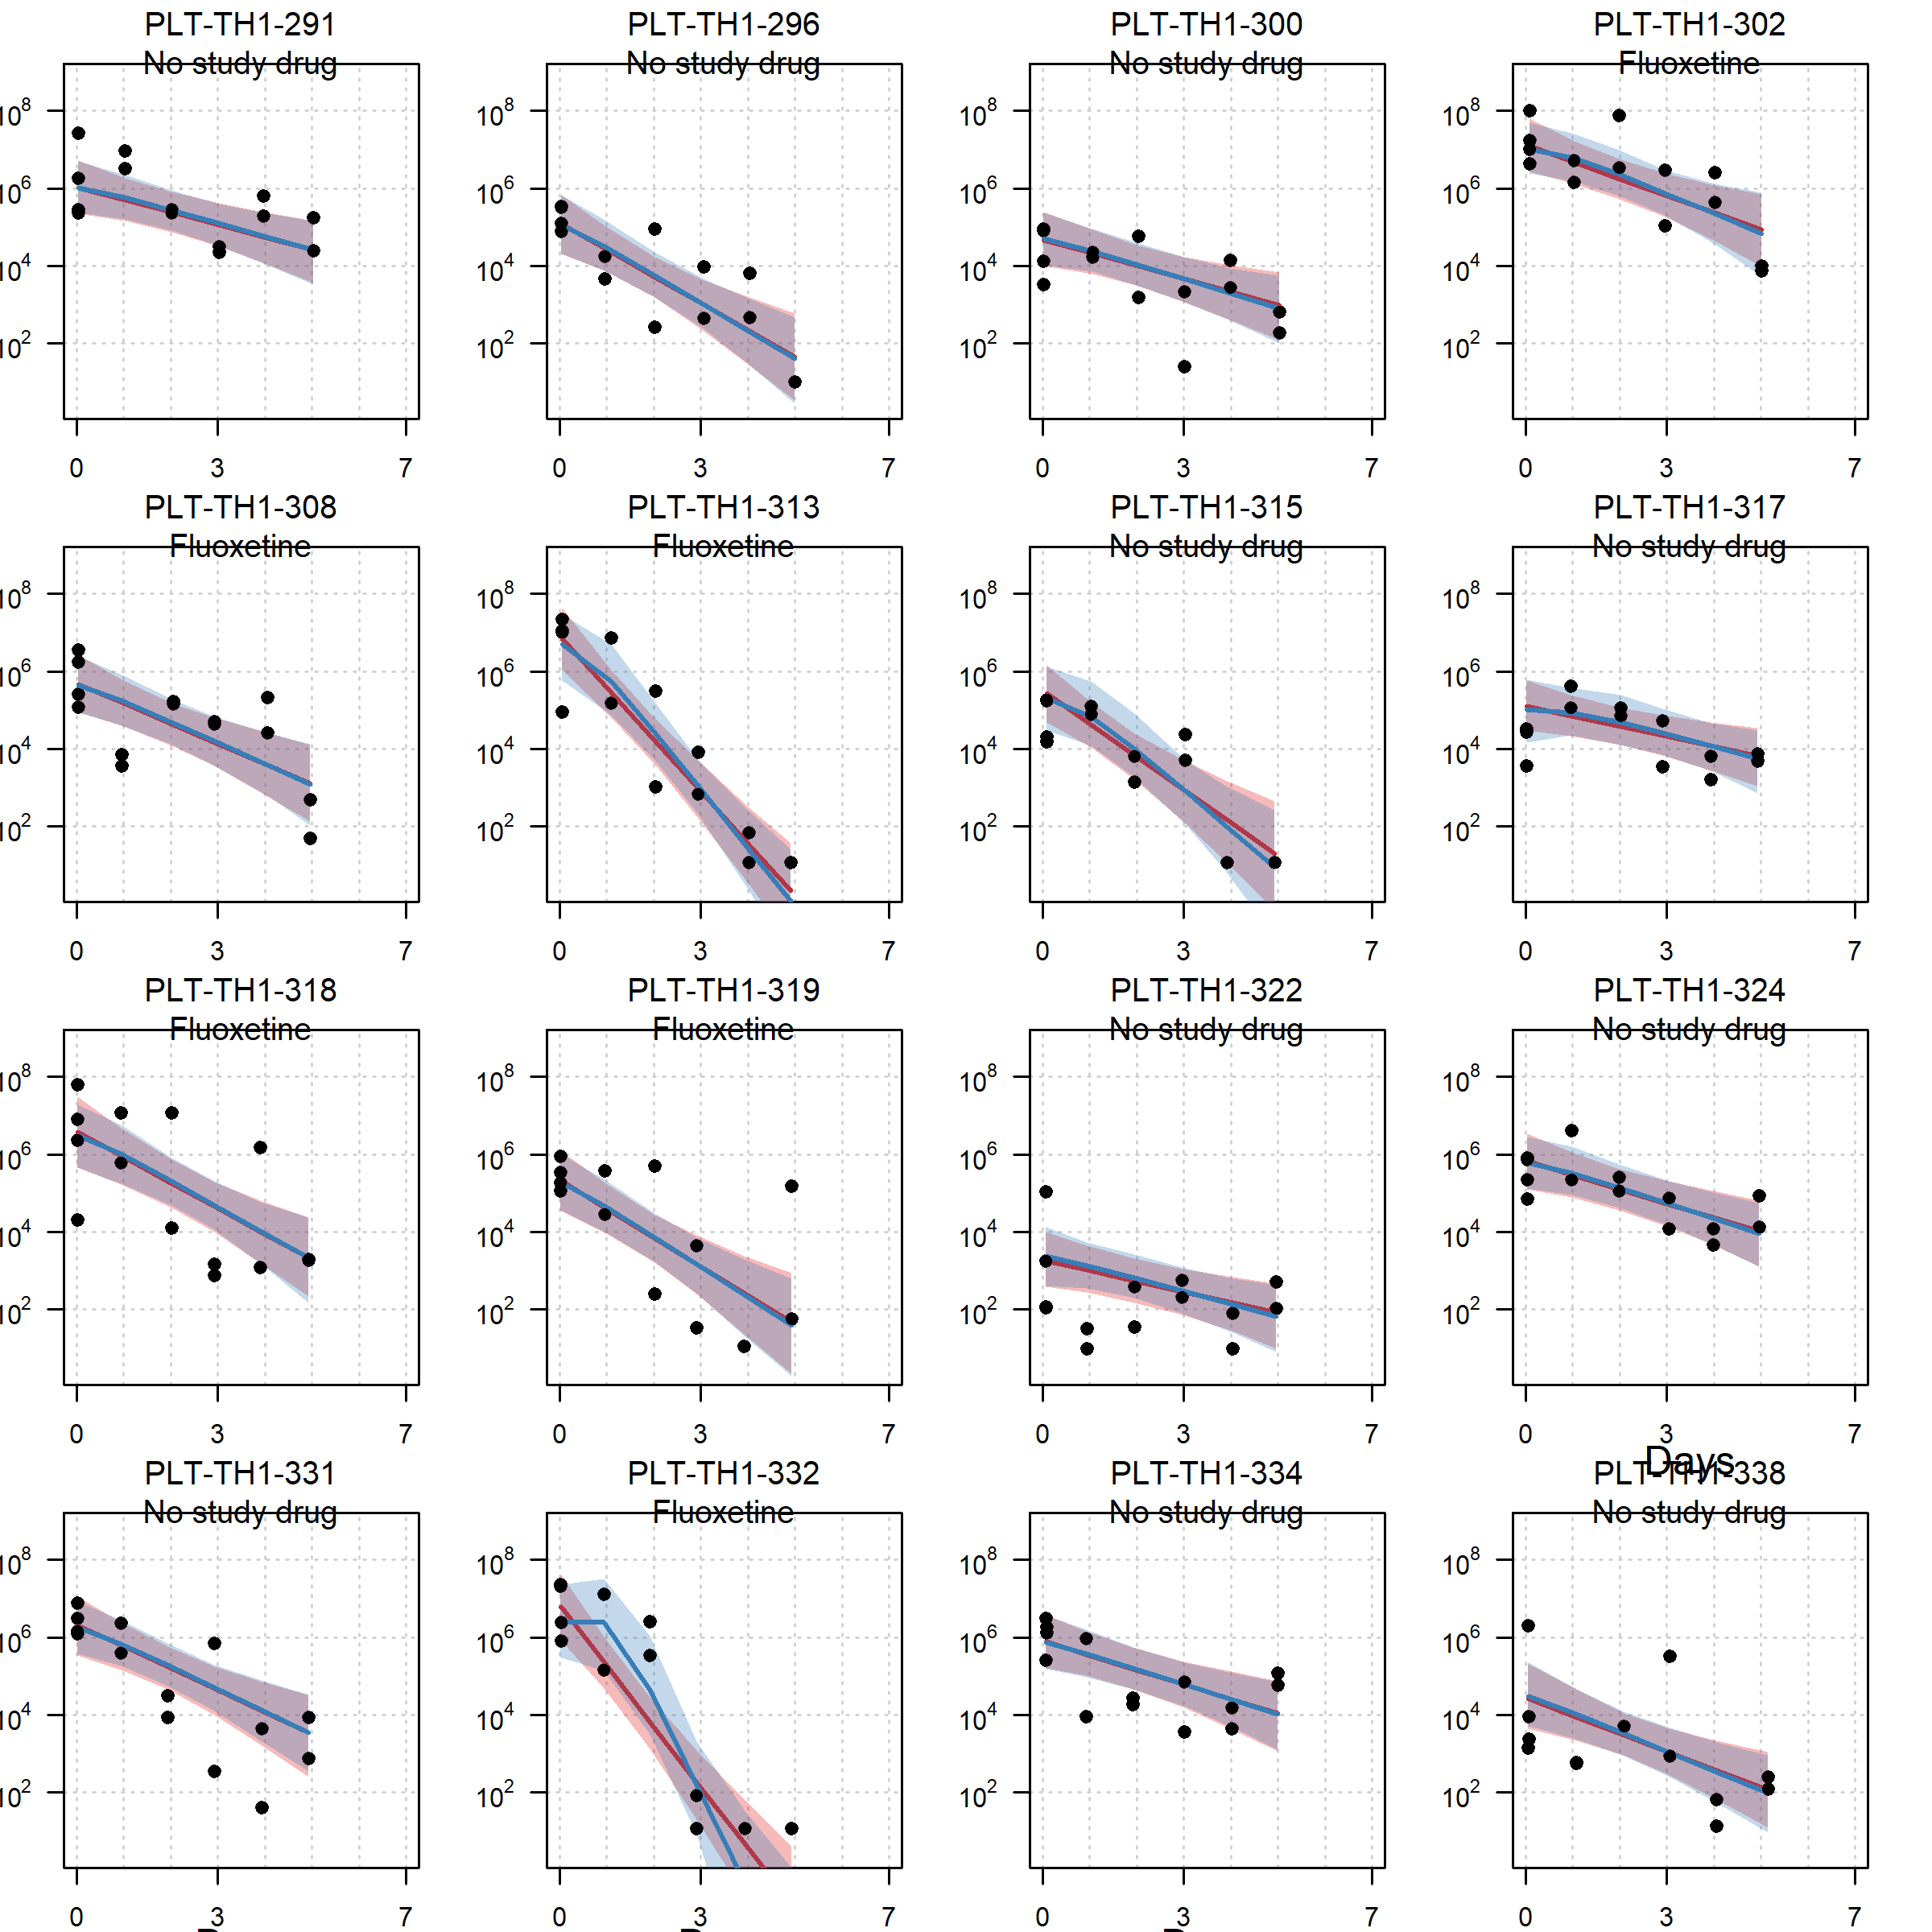
\includegraphics{Fluoxetine_analysis_files/figure-pdf/individ_data-6.png}

}

\end{figure}

\begin{figure}[H]

{\centering 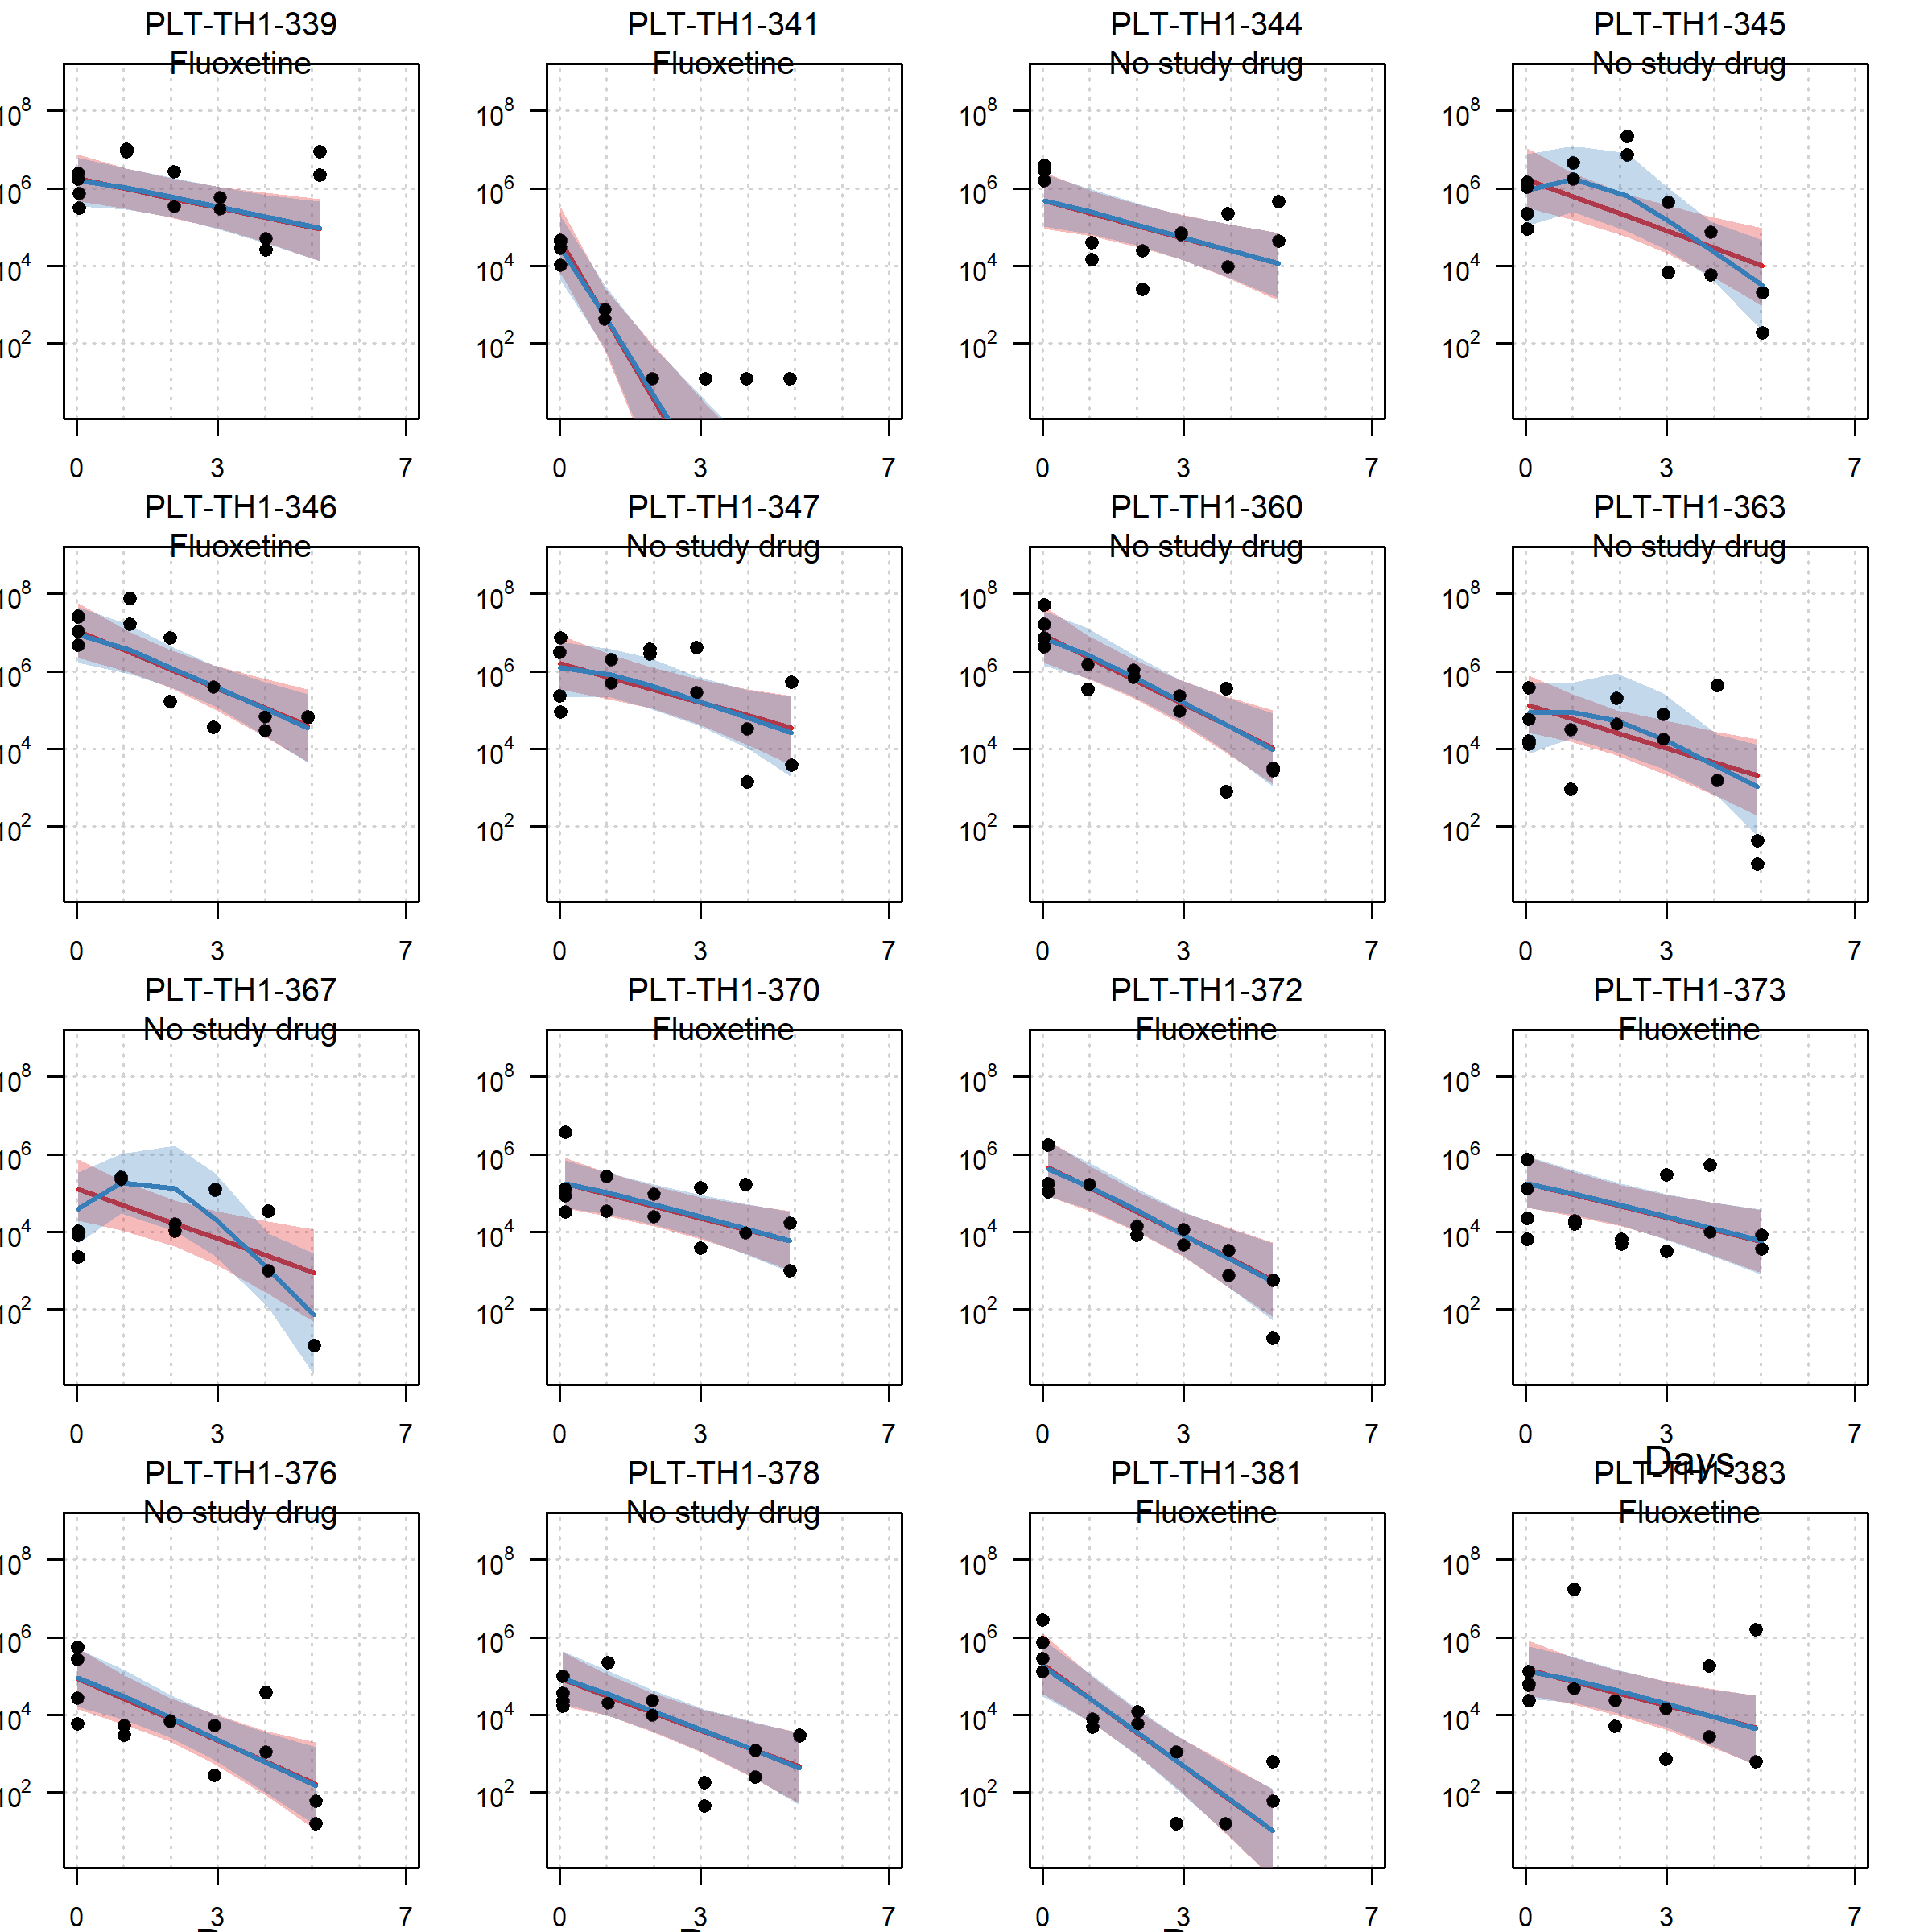
\includegraphics{Fluoxetine_analysis_files/figure-pdf/individ_data-7.png}

}

\end{figure}

\begin{figure}[H]

{\centering 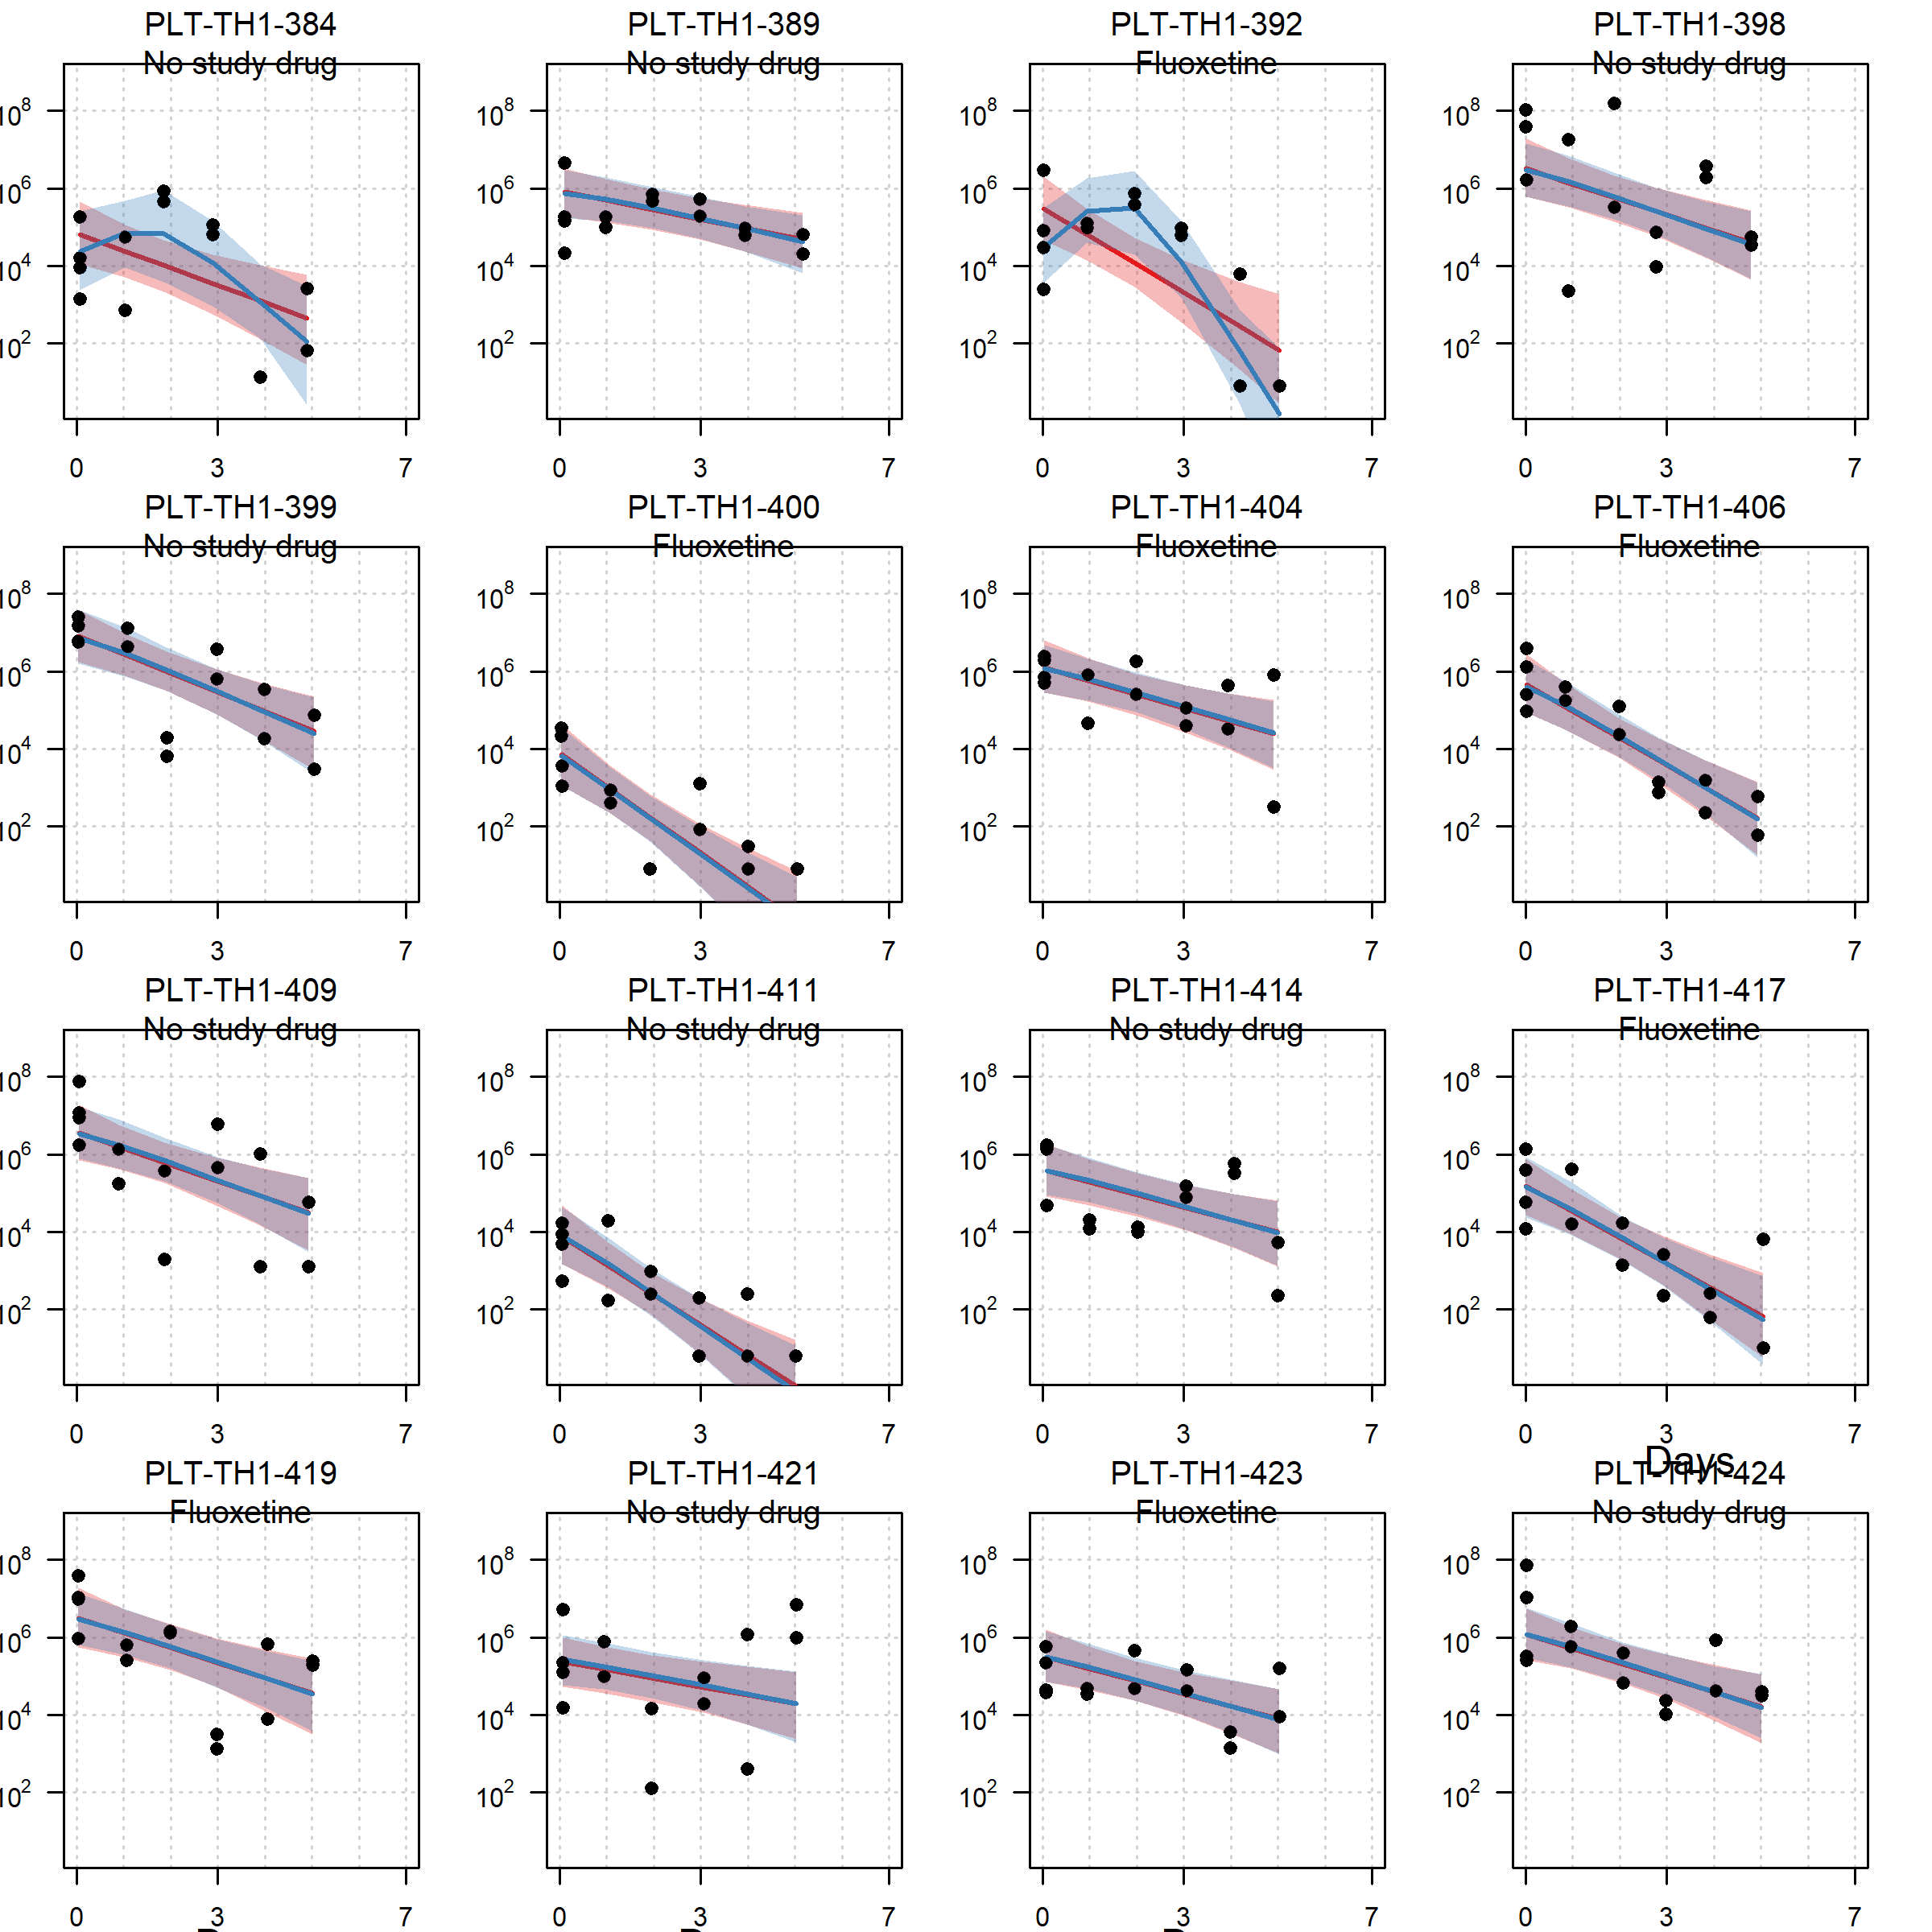
\includegraphics{Fluoxetine_analysis_files/figure-pdf/individ_data-8.png}

}

\end{figure}

\begin{figure}[H]

{\centering 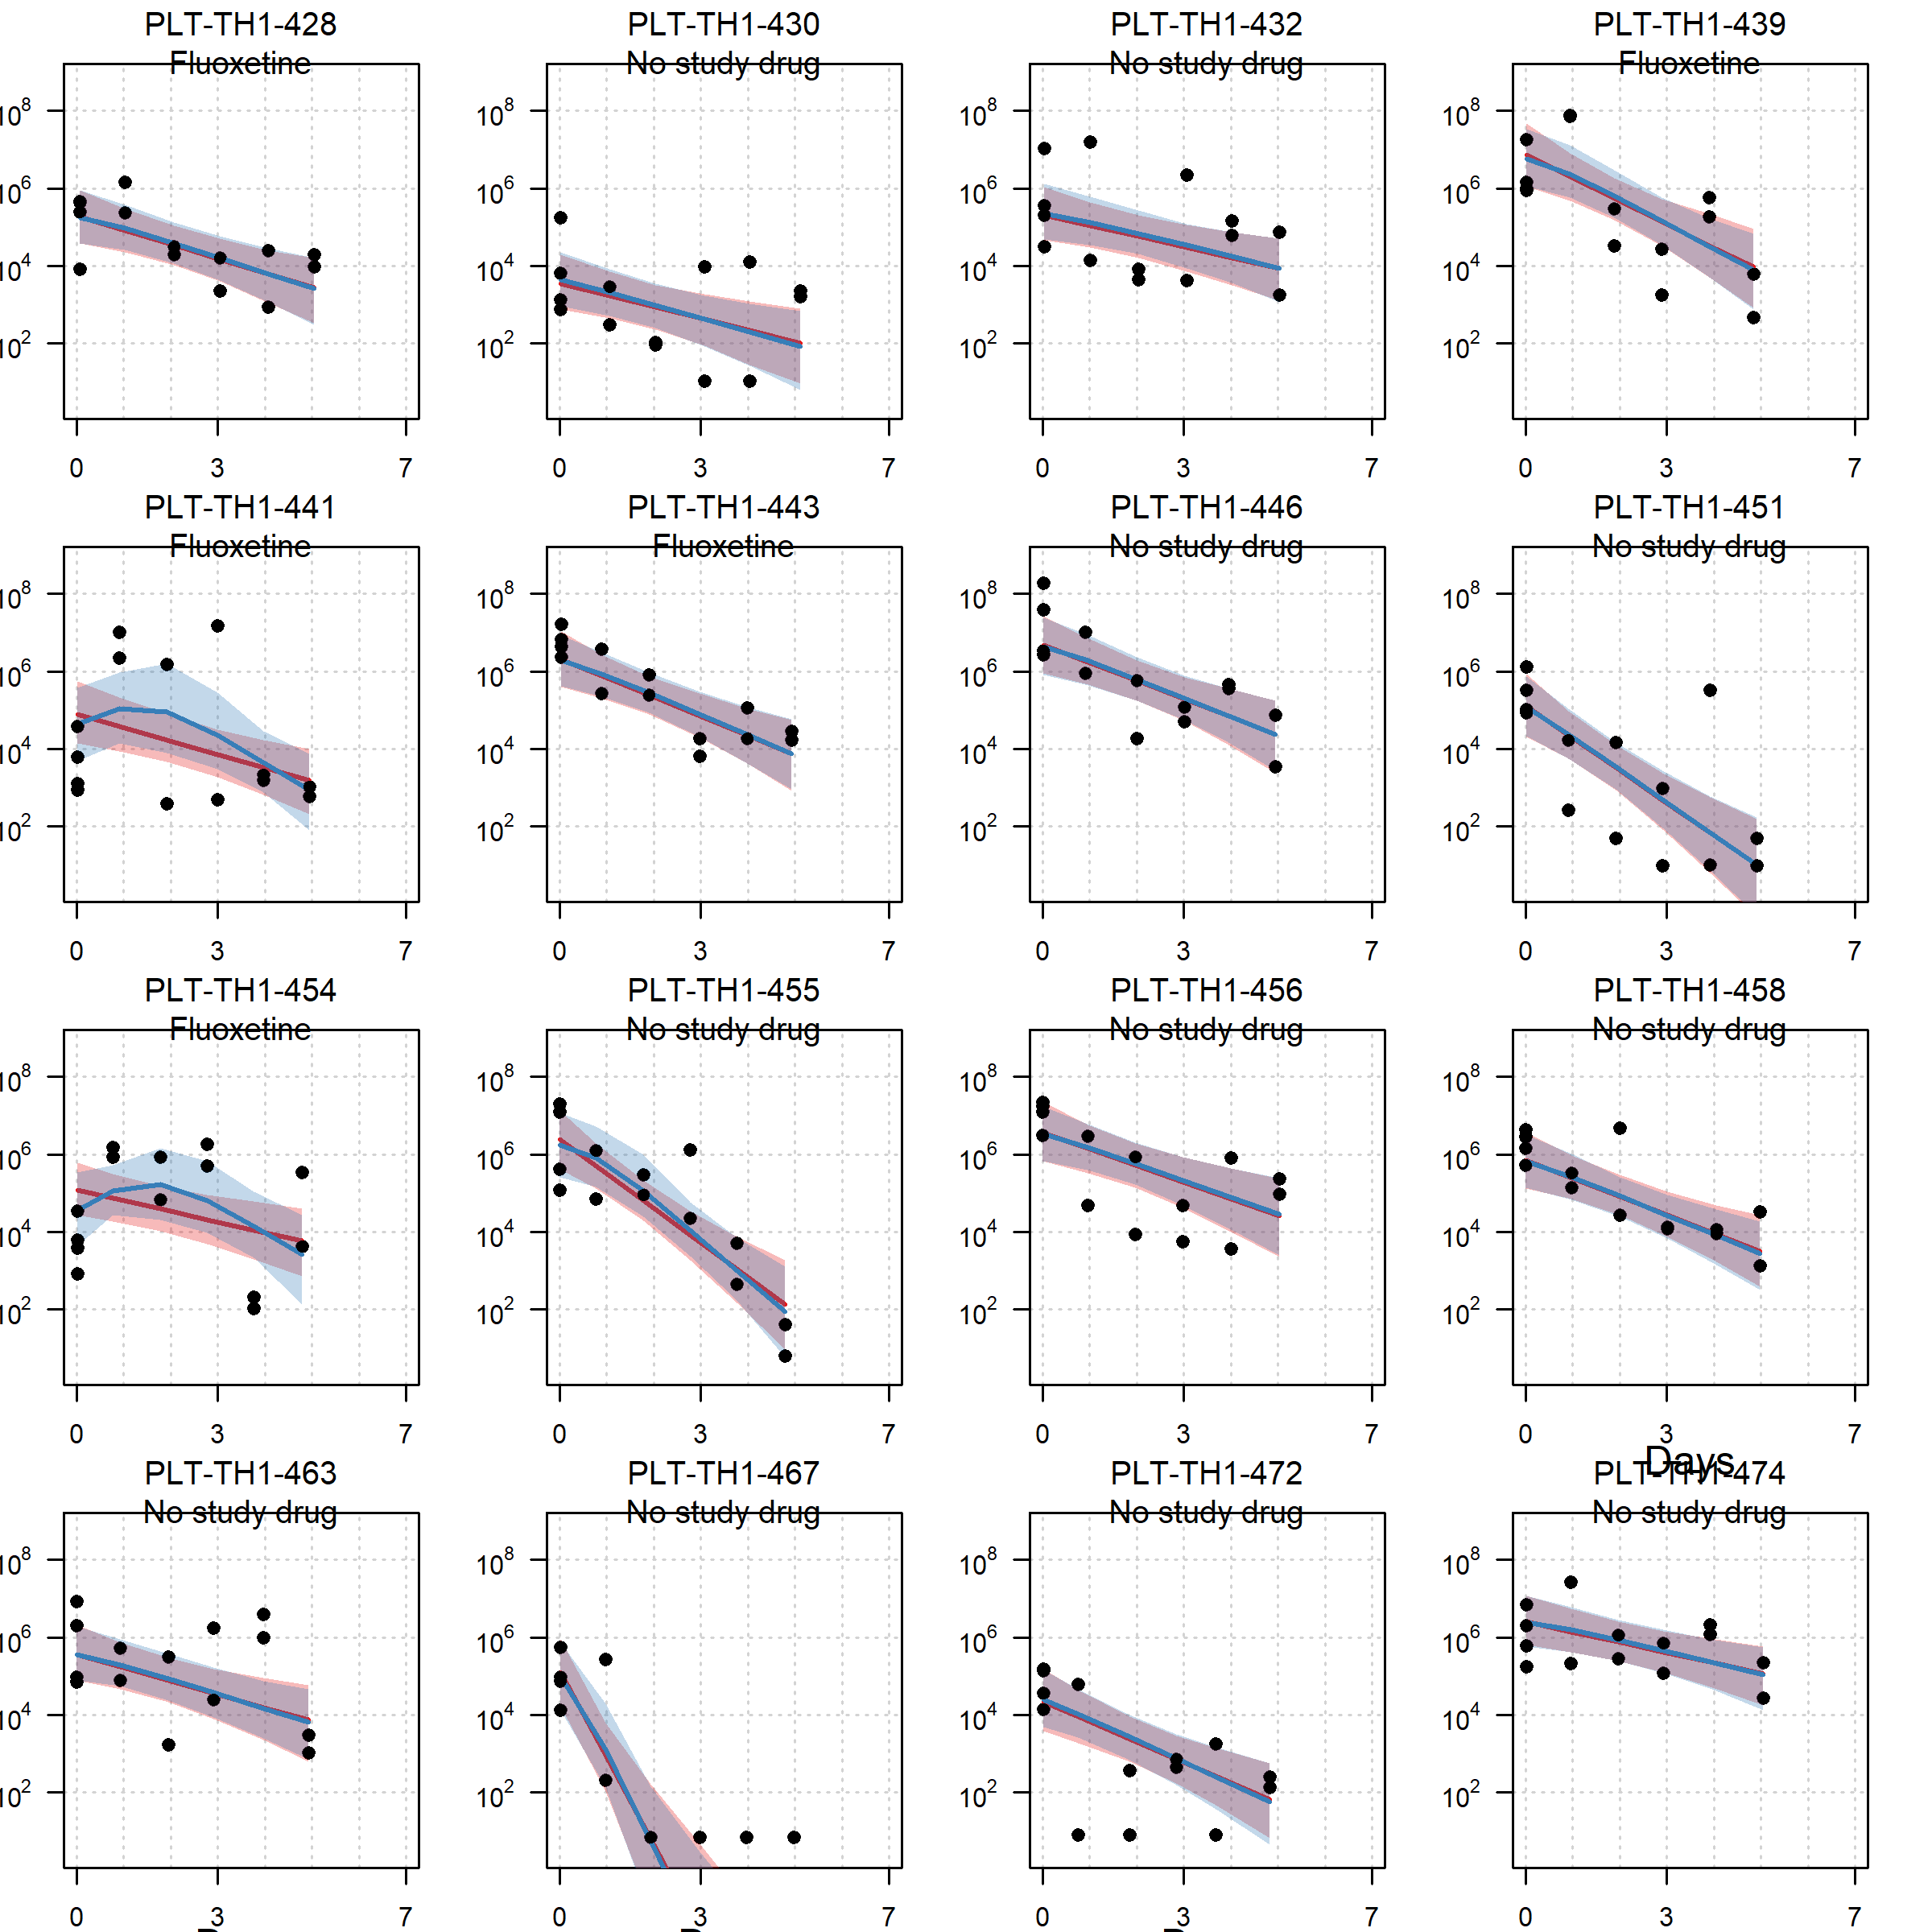
\includegraphics{Fluoxetine_analysis_files/figure-pdf/individ_data-9.png}

}

\end{figure}

\begin{figure}[H]

{\centering 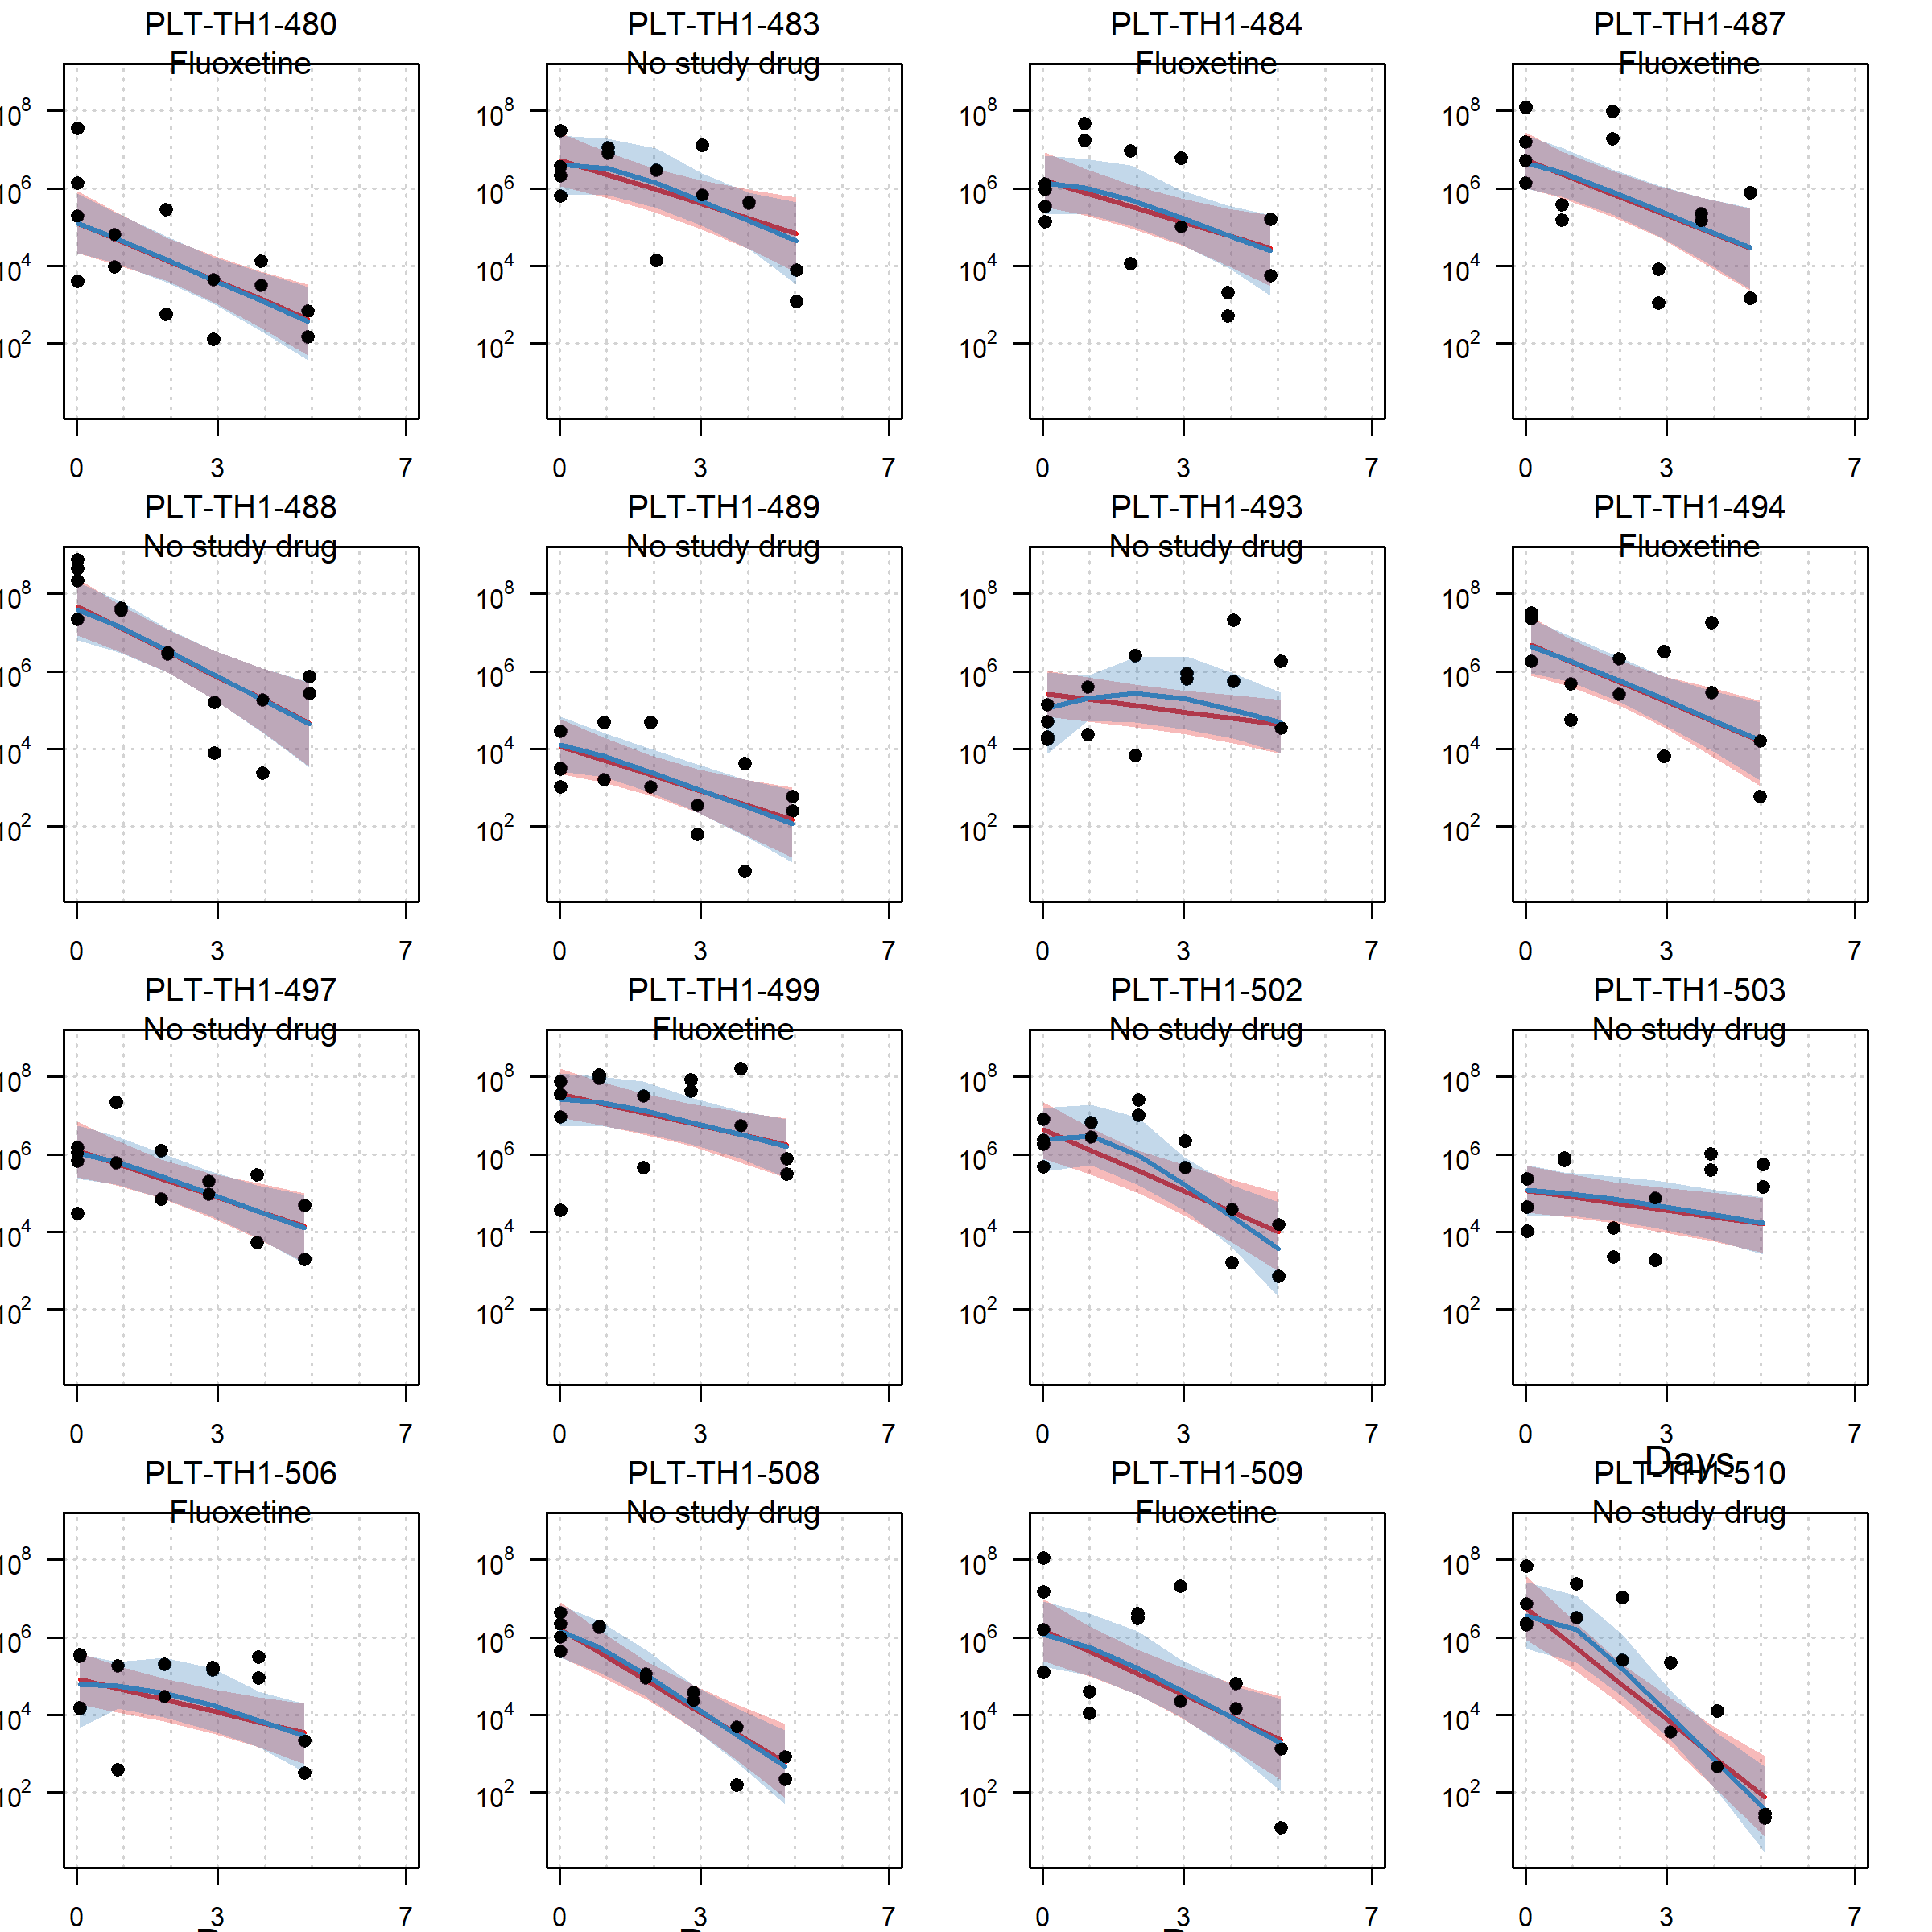
\includegraphics{Fluoxetine_analysis_files/figure-pdf/individ_data-10.png}

}

\end{figure}

\begin{figure}[H]

{\centering 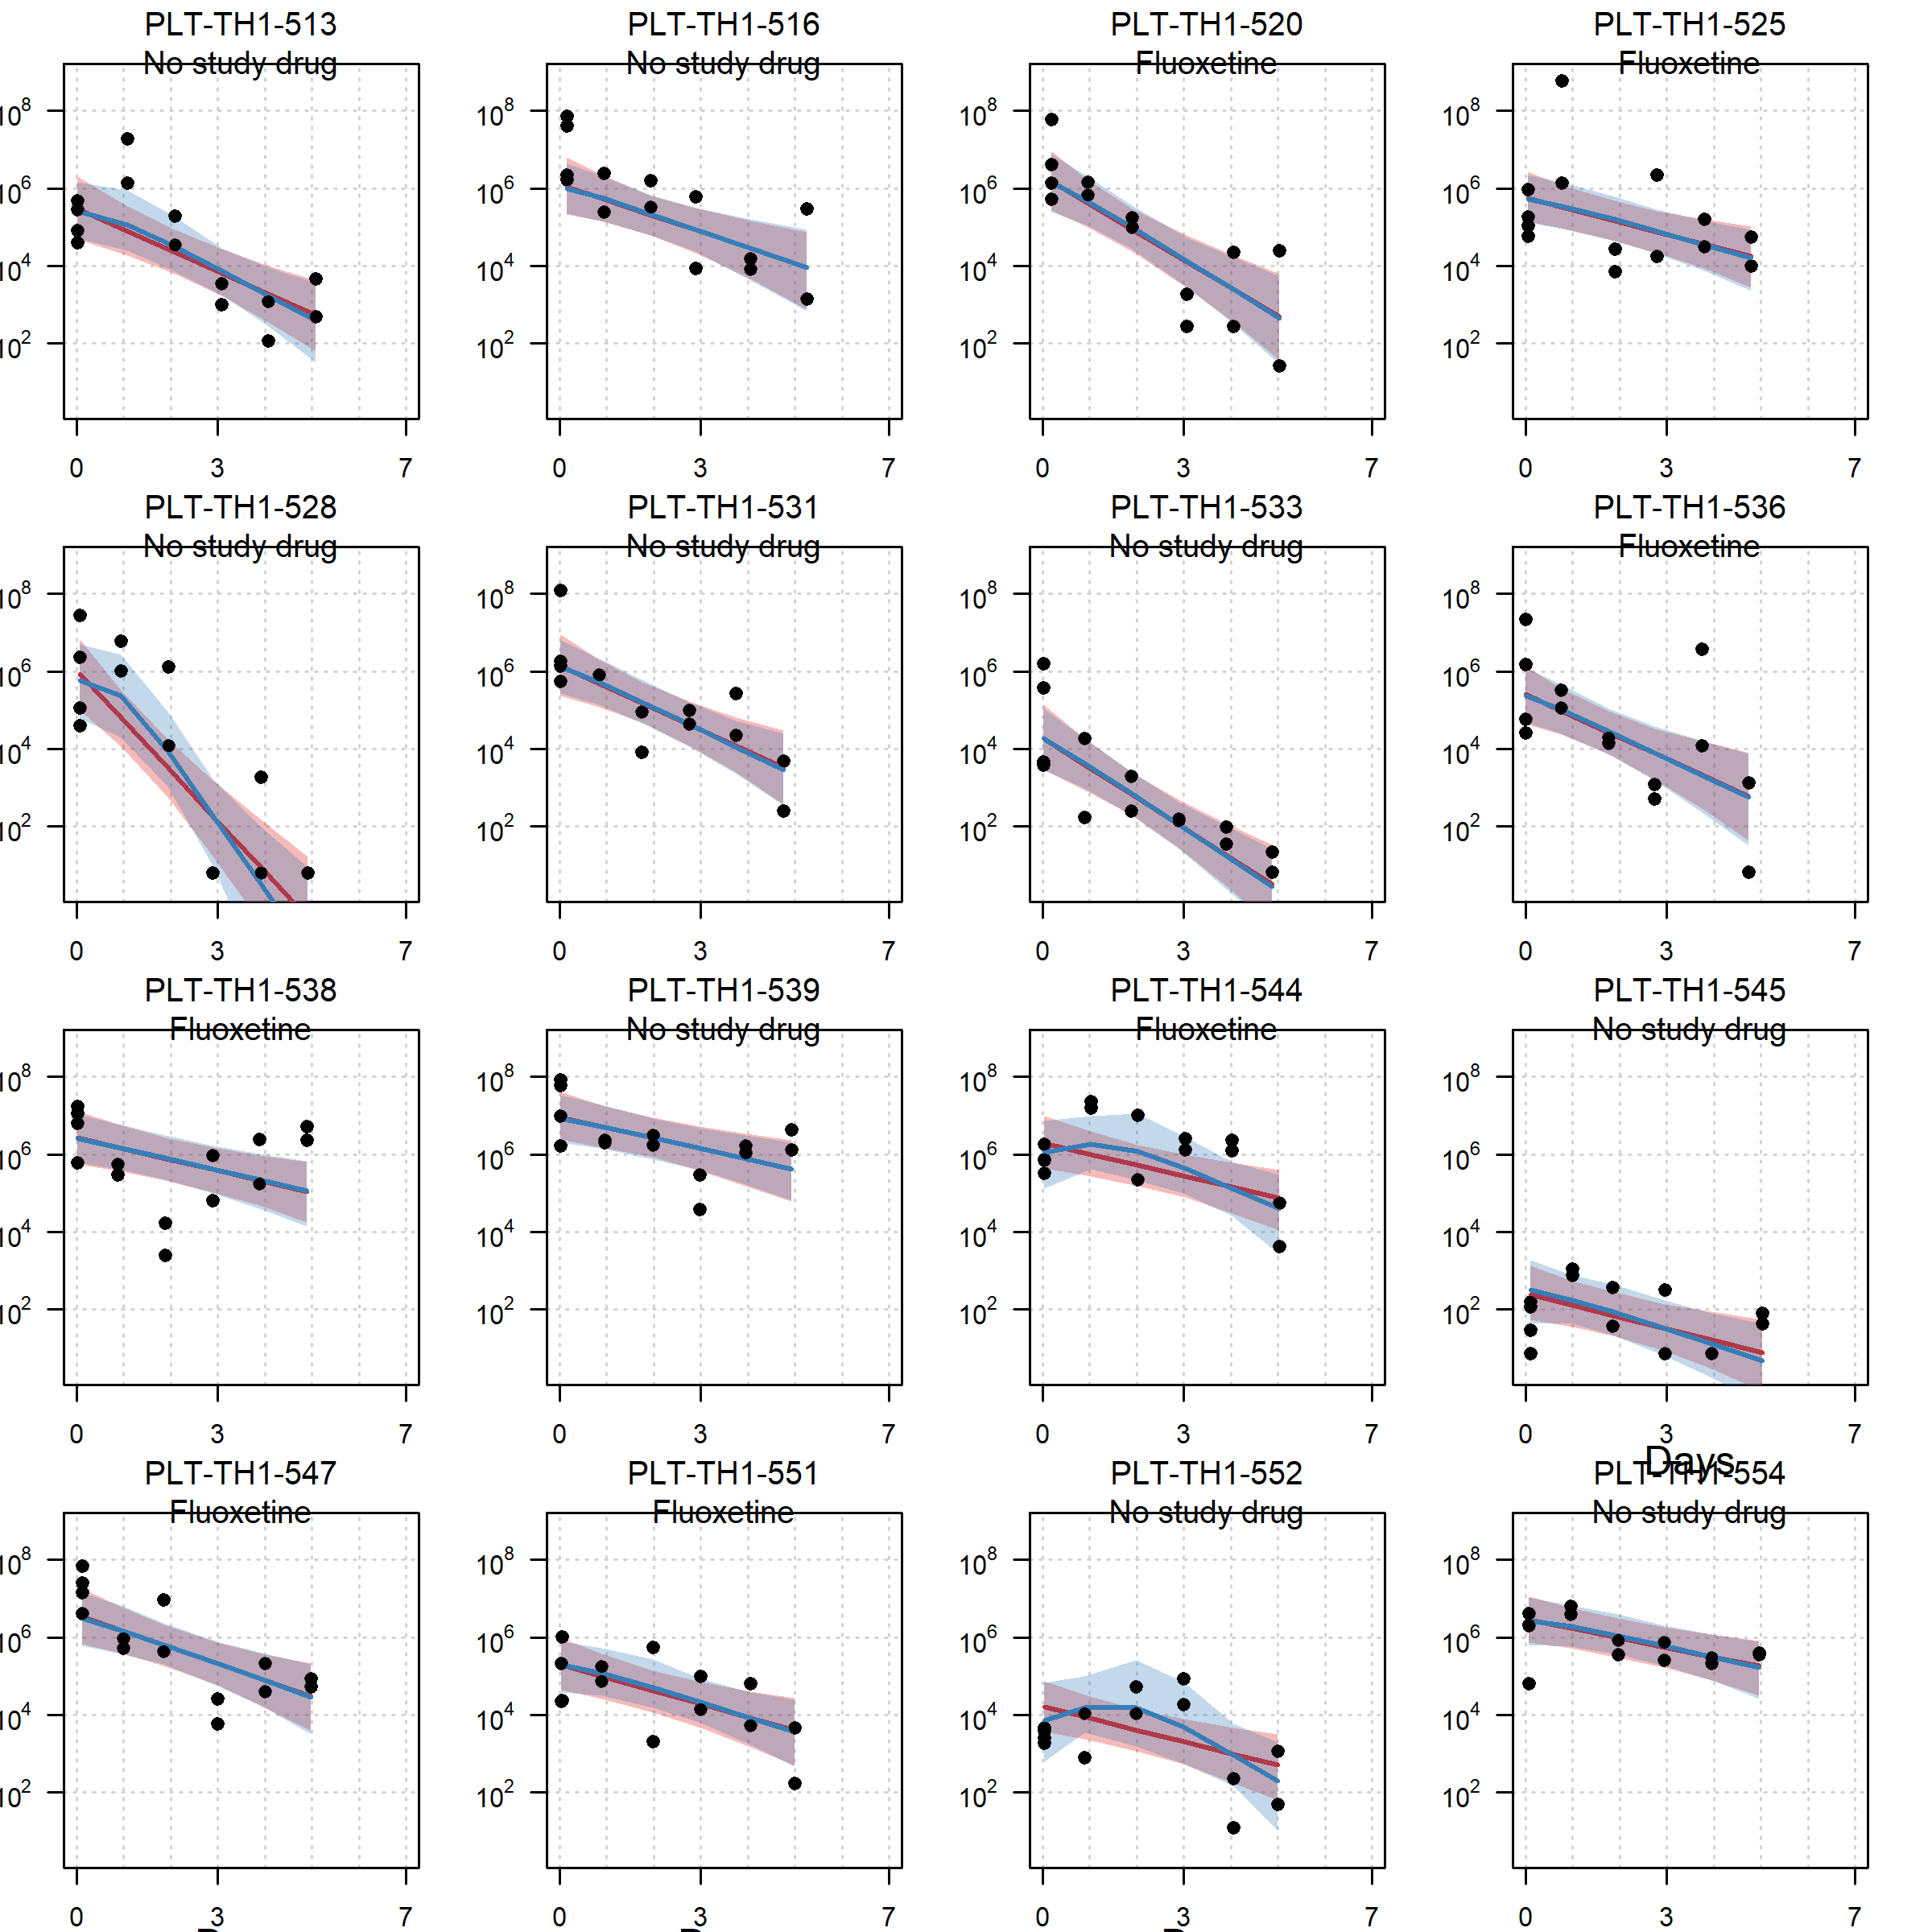
\includegraphics{Fluoxetine_analysis_files/figure-pdf/individ_data-11.png}

}

\end{figure}

\begin{figure}[H]

{\centering 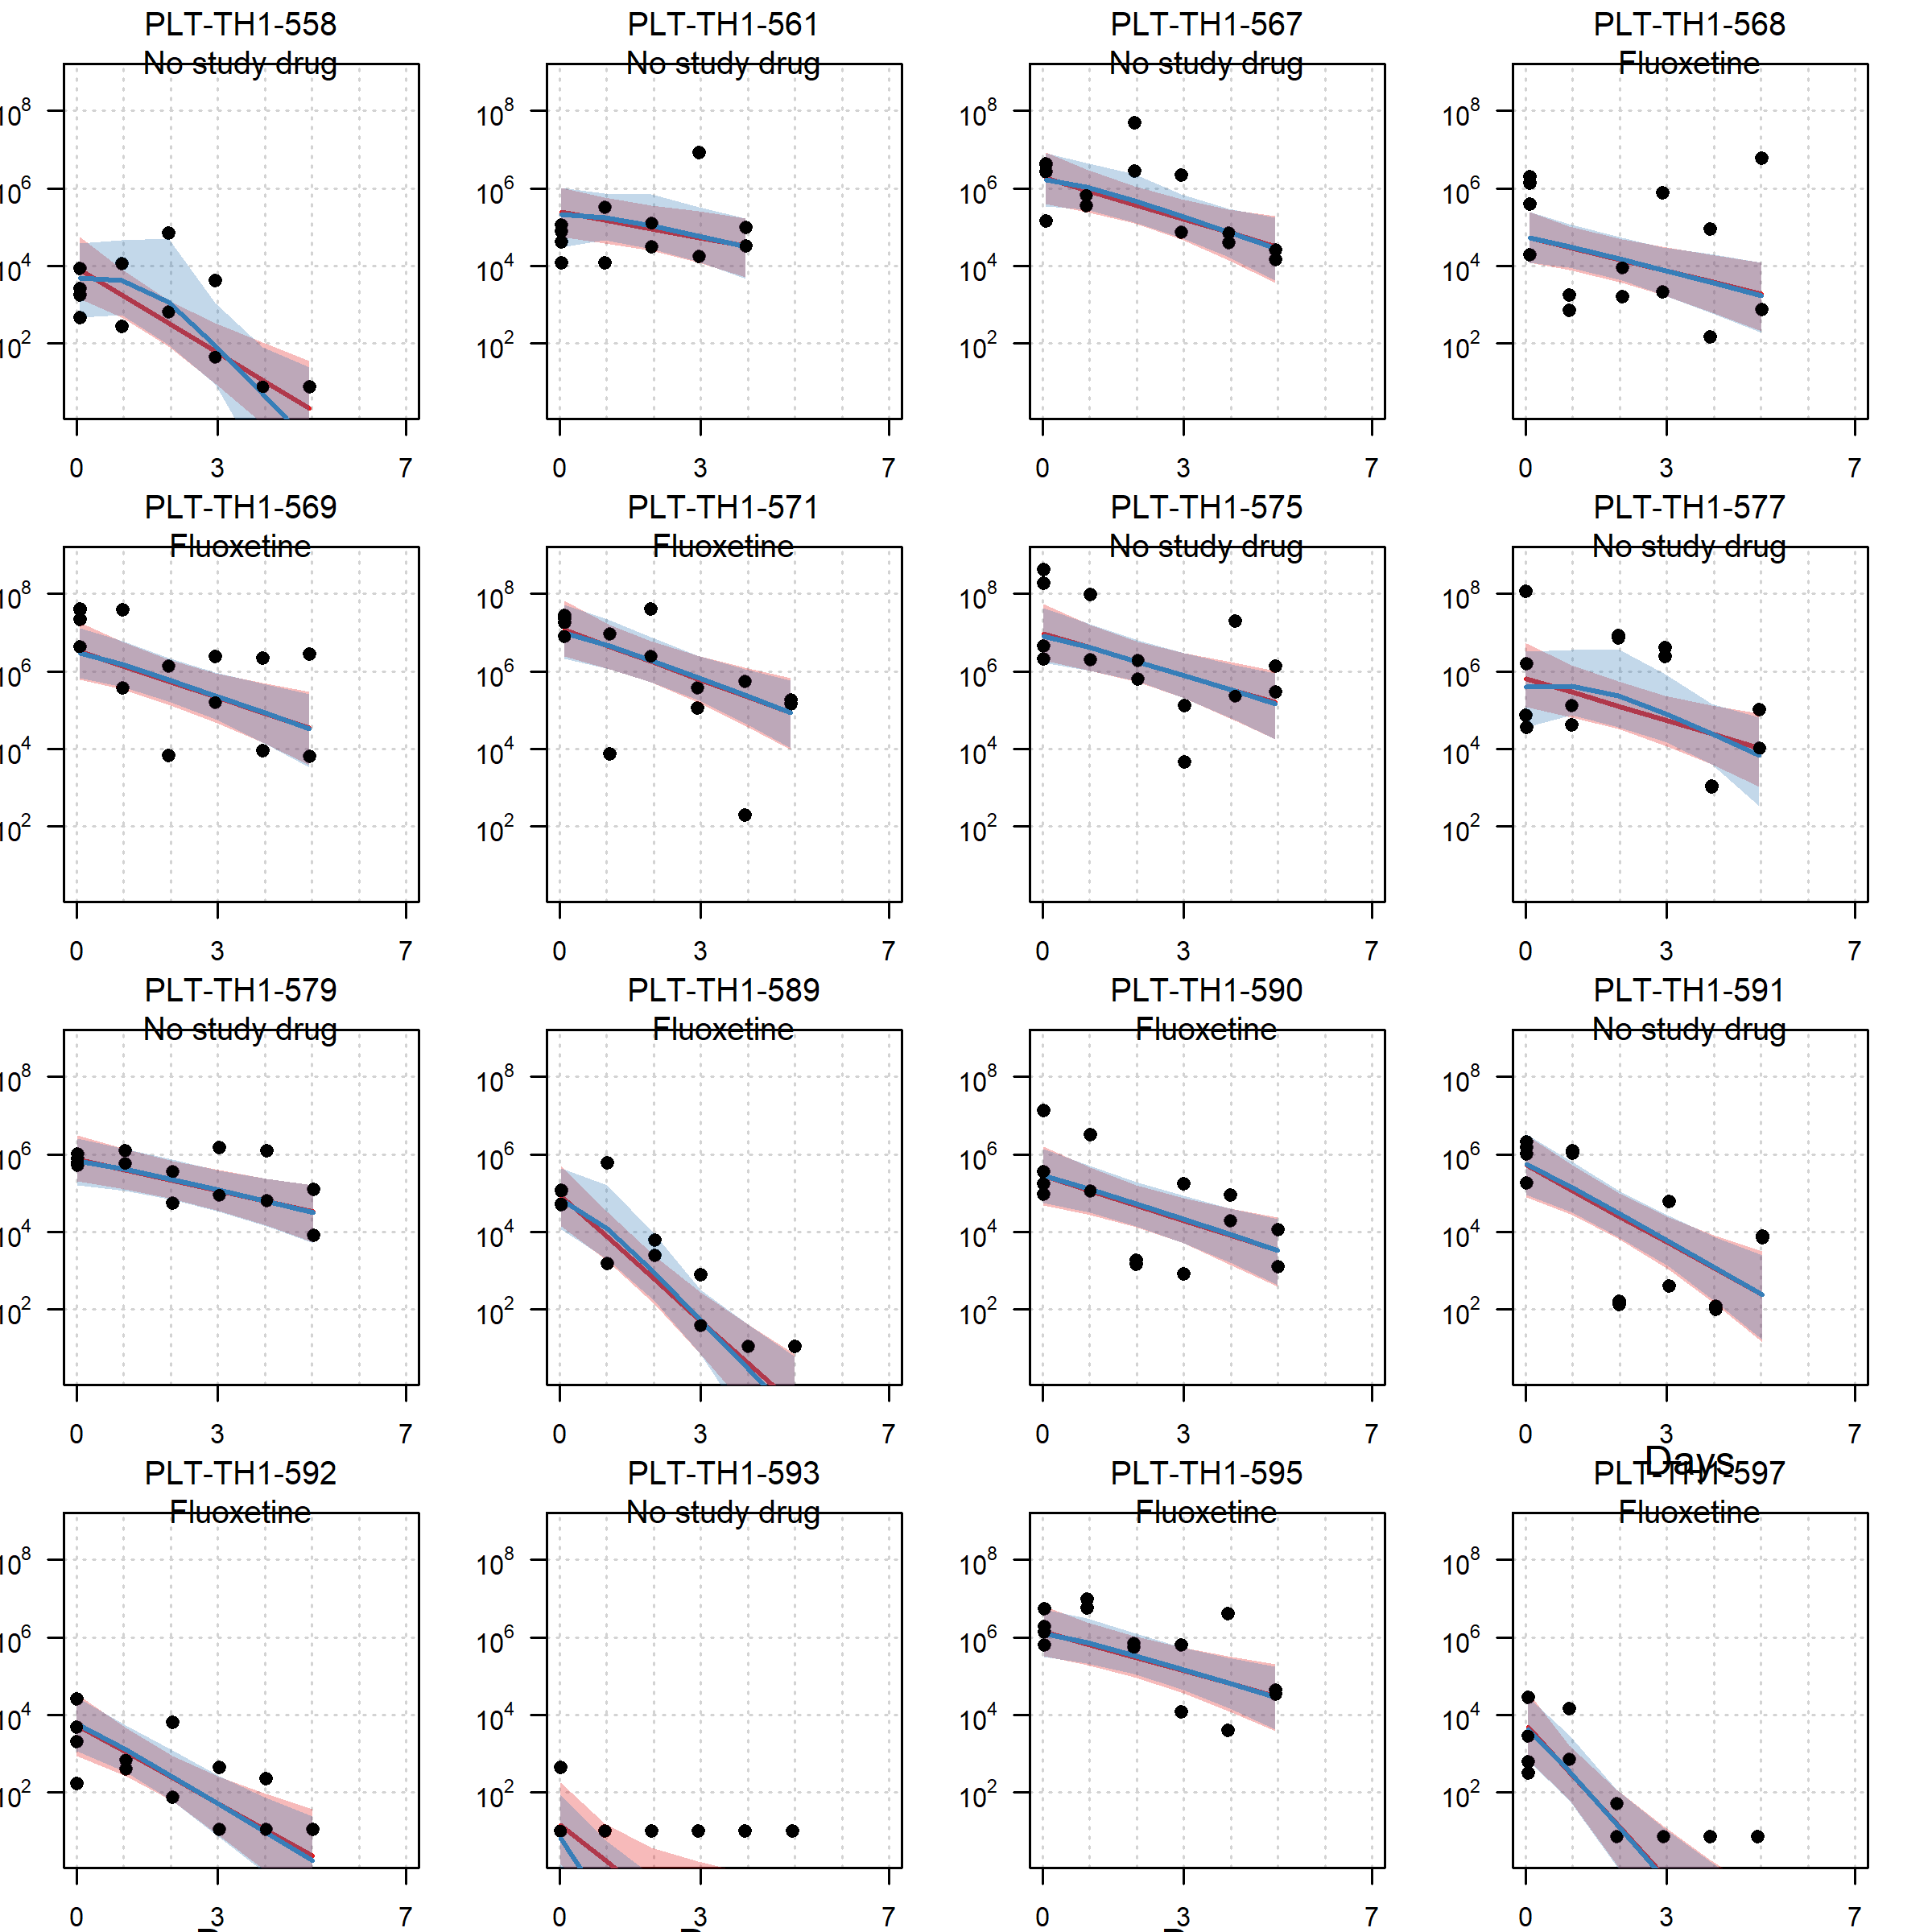
\includegraphics{Fluoxetine_analysis_files/figure-pdf/individ_data-12.png}

}

\end{figure}

\begin{figure}[H]

{\centering 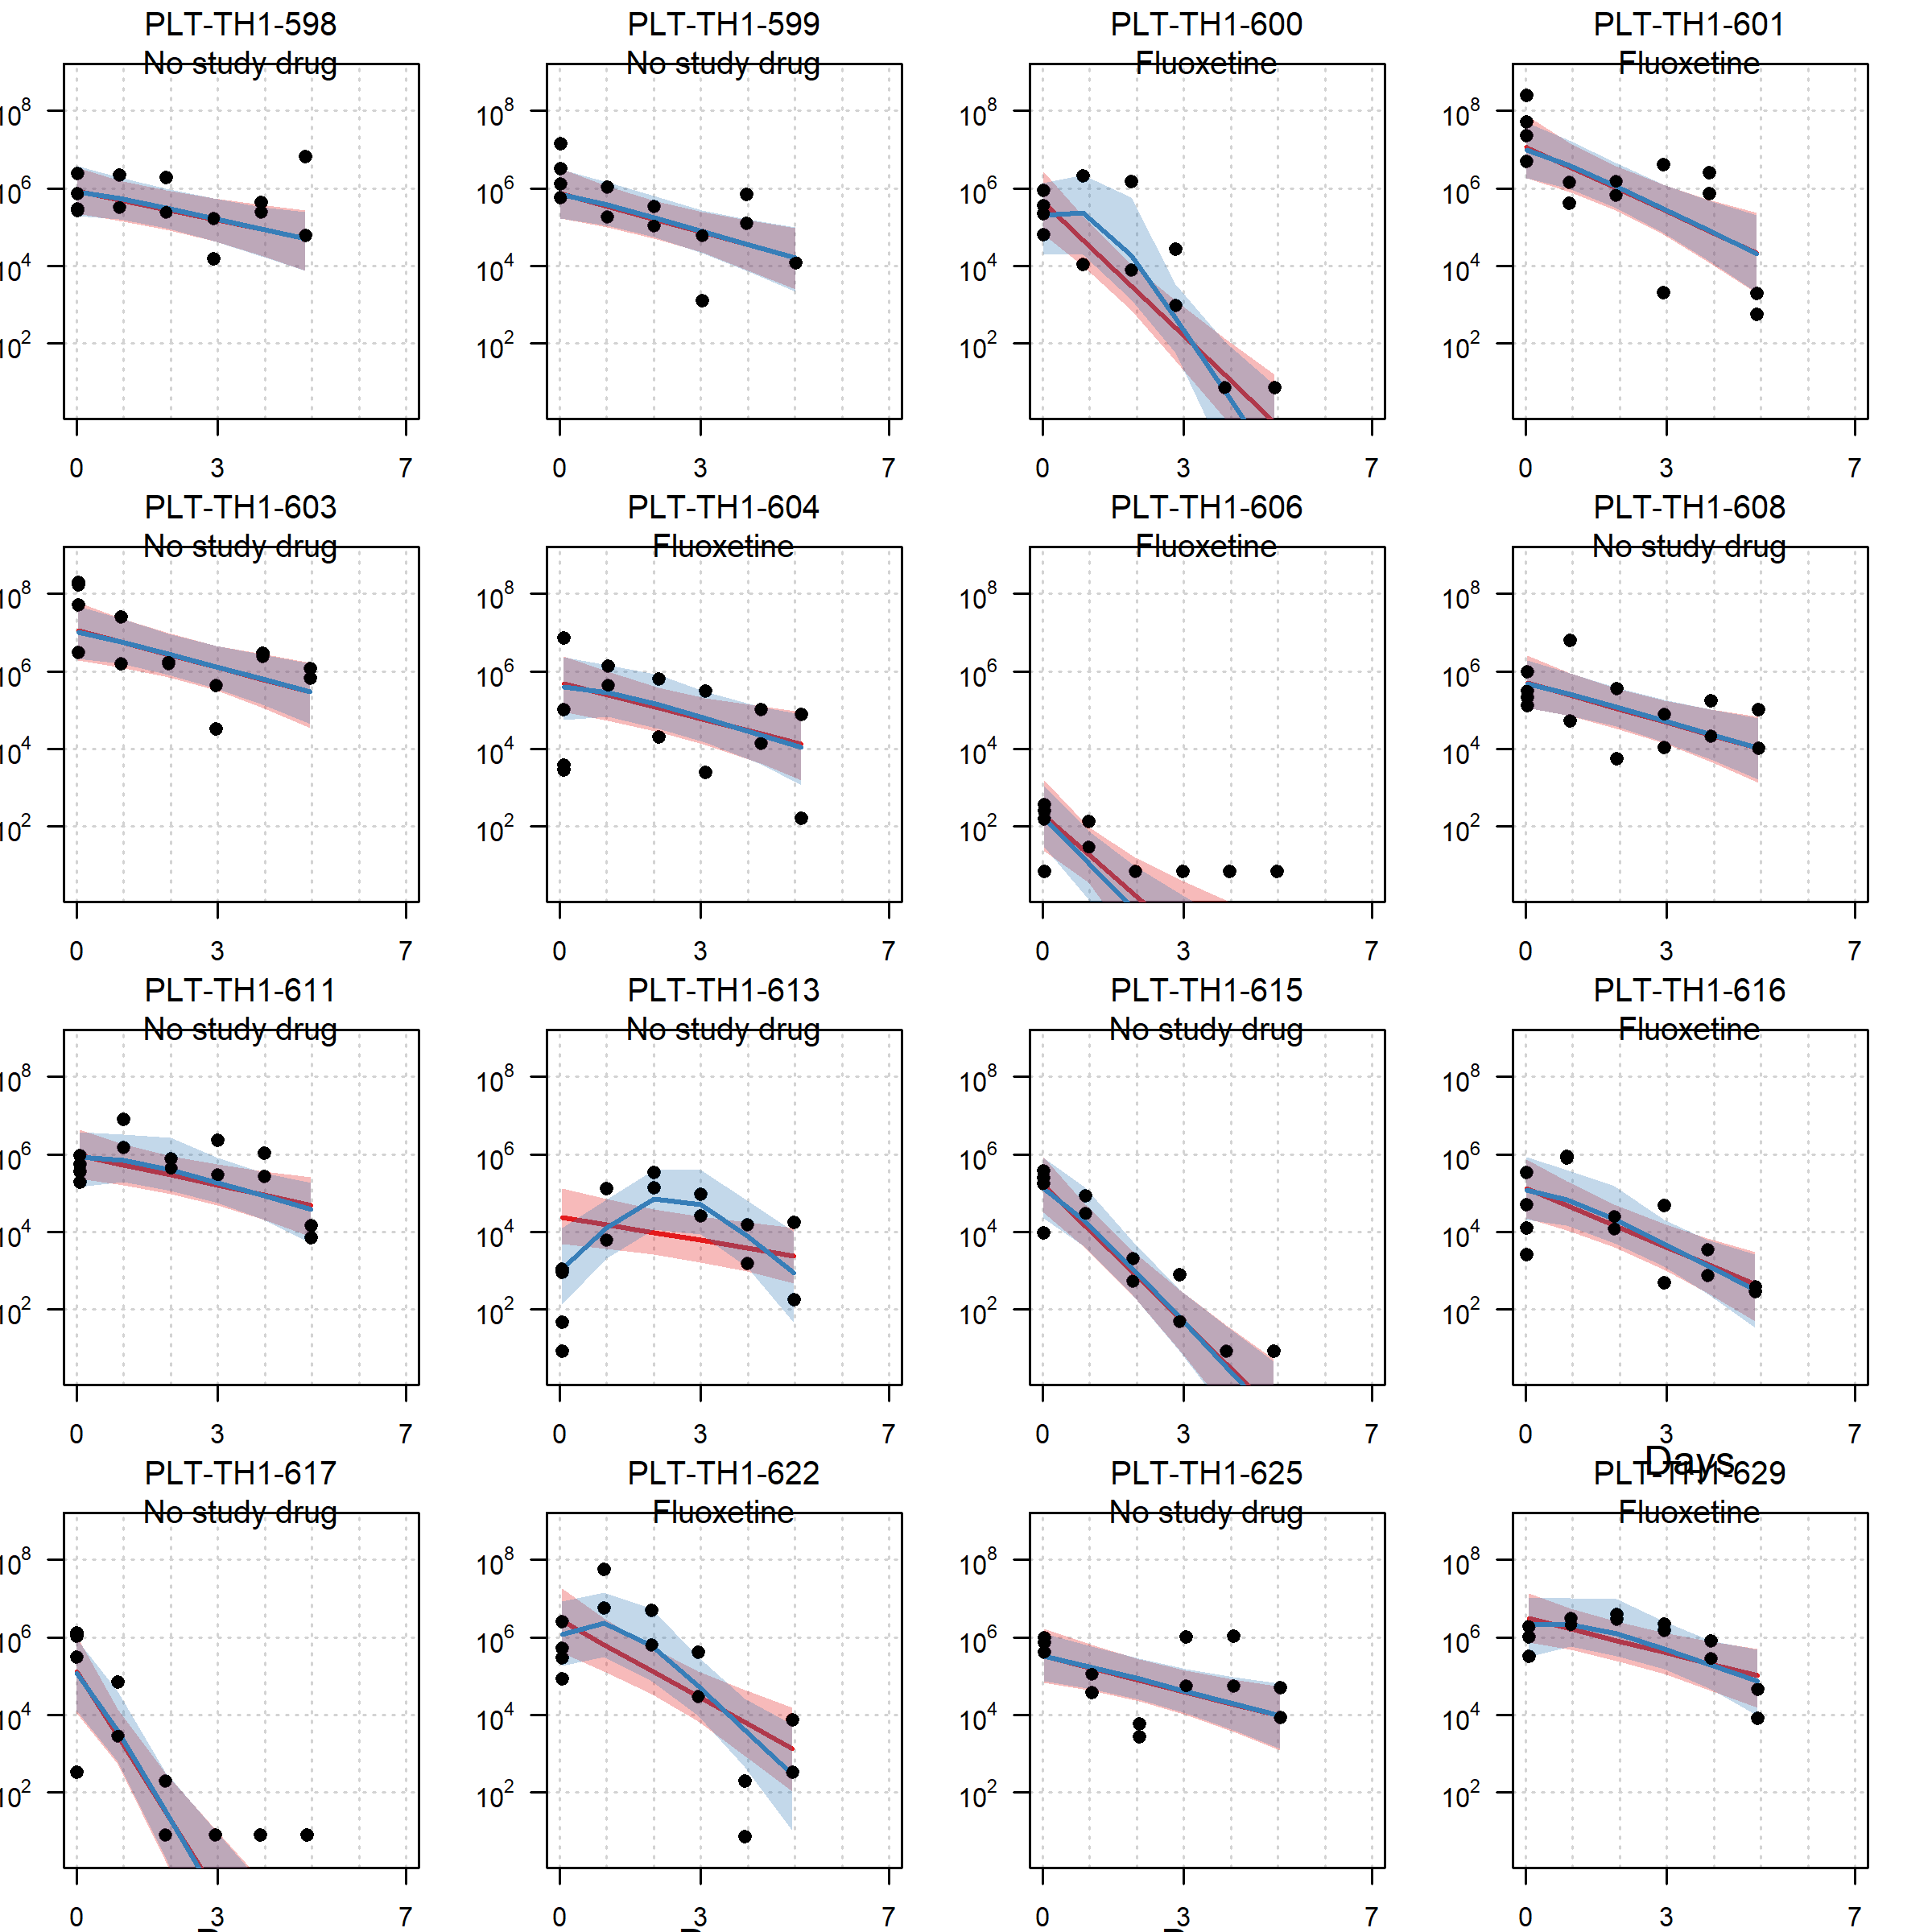
\includegraphics{Fluoxetine_analysis_files/figure-pdf/individ_data-13.png}

}

\end{figure}

\begin{figure}[H]

{\centering 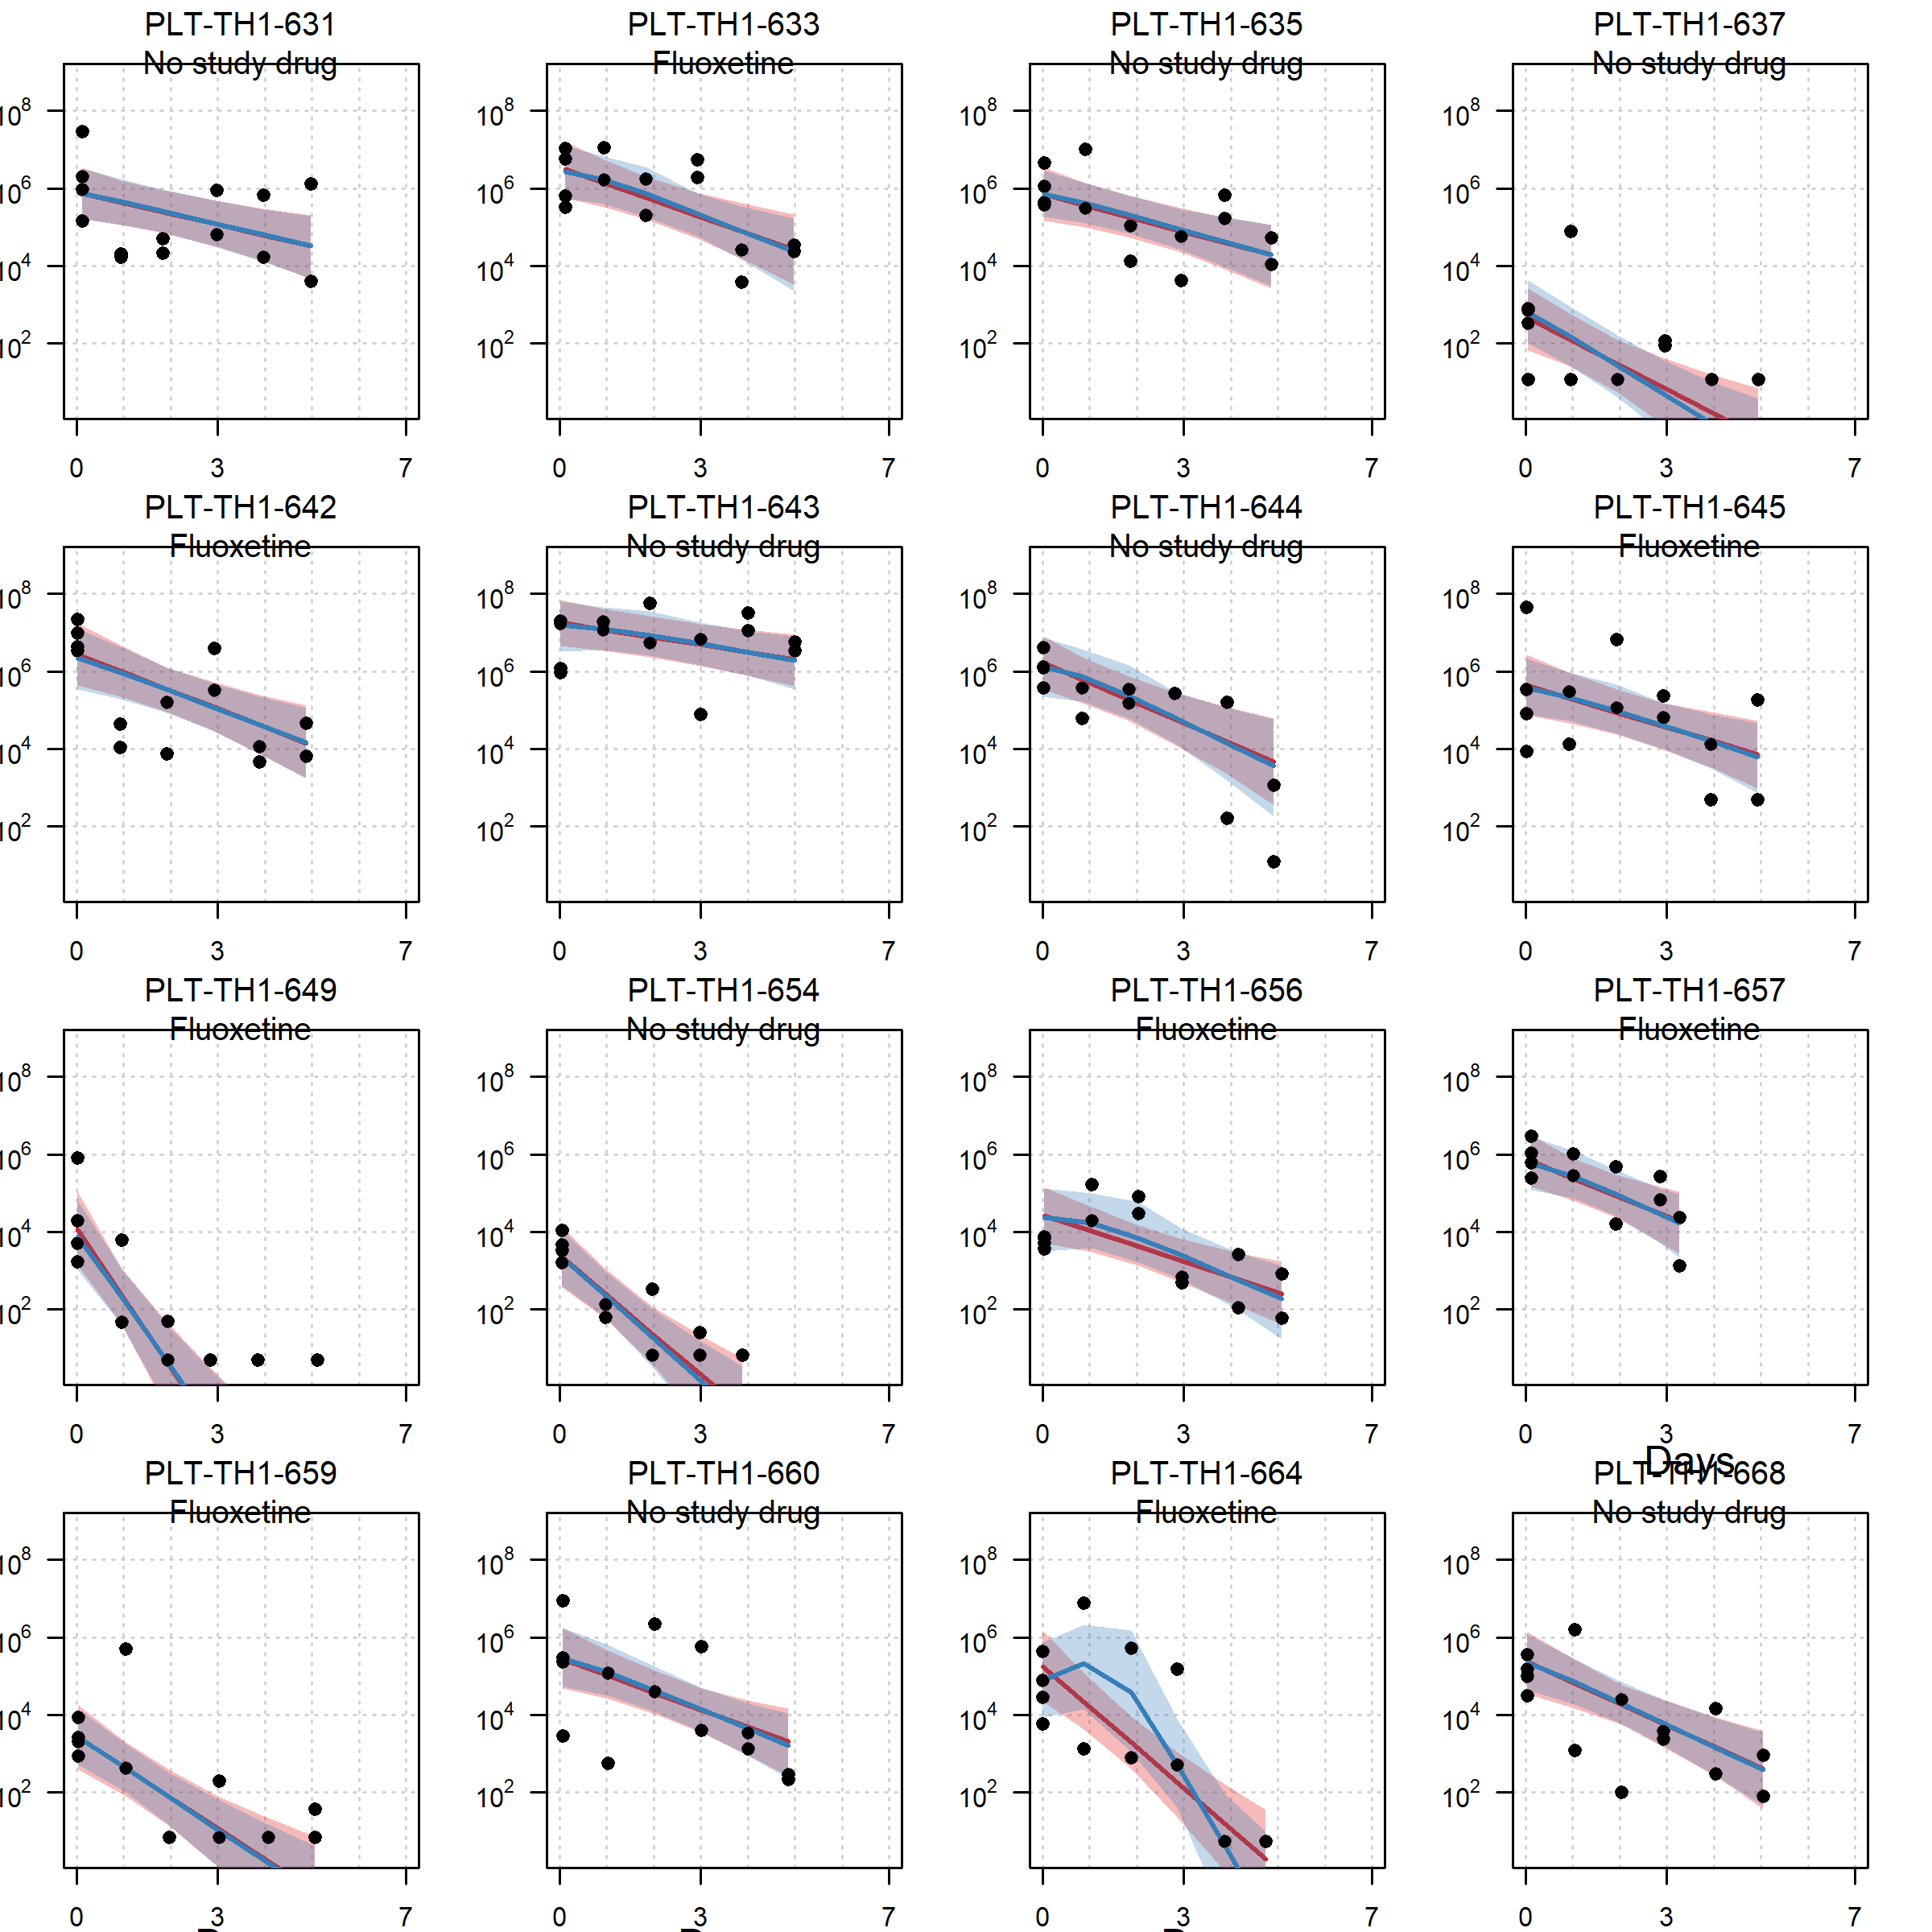
\includegraphics{Fluoxetine_analysis_files/figure-pdf/individ_data-14.png}

}

\end{figure}

\begin{figure}[H]

{\centering 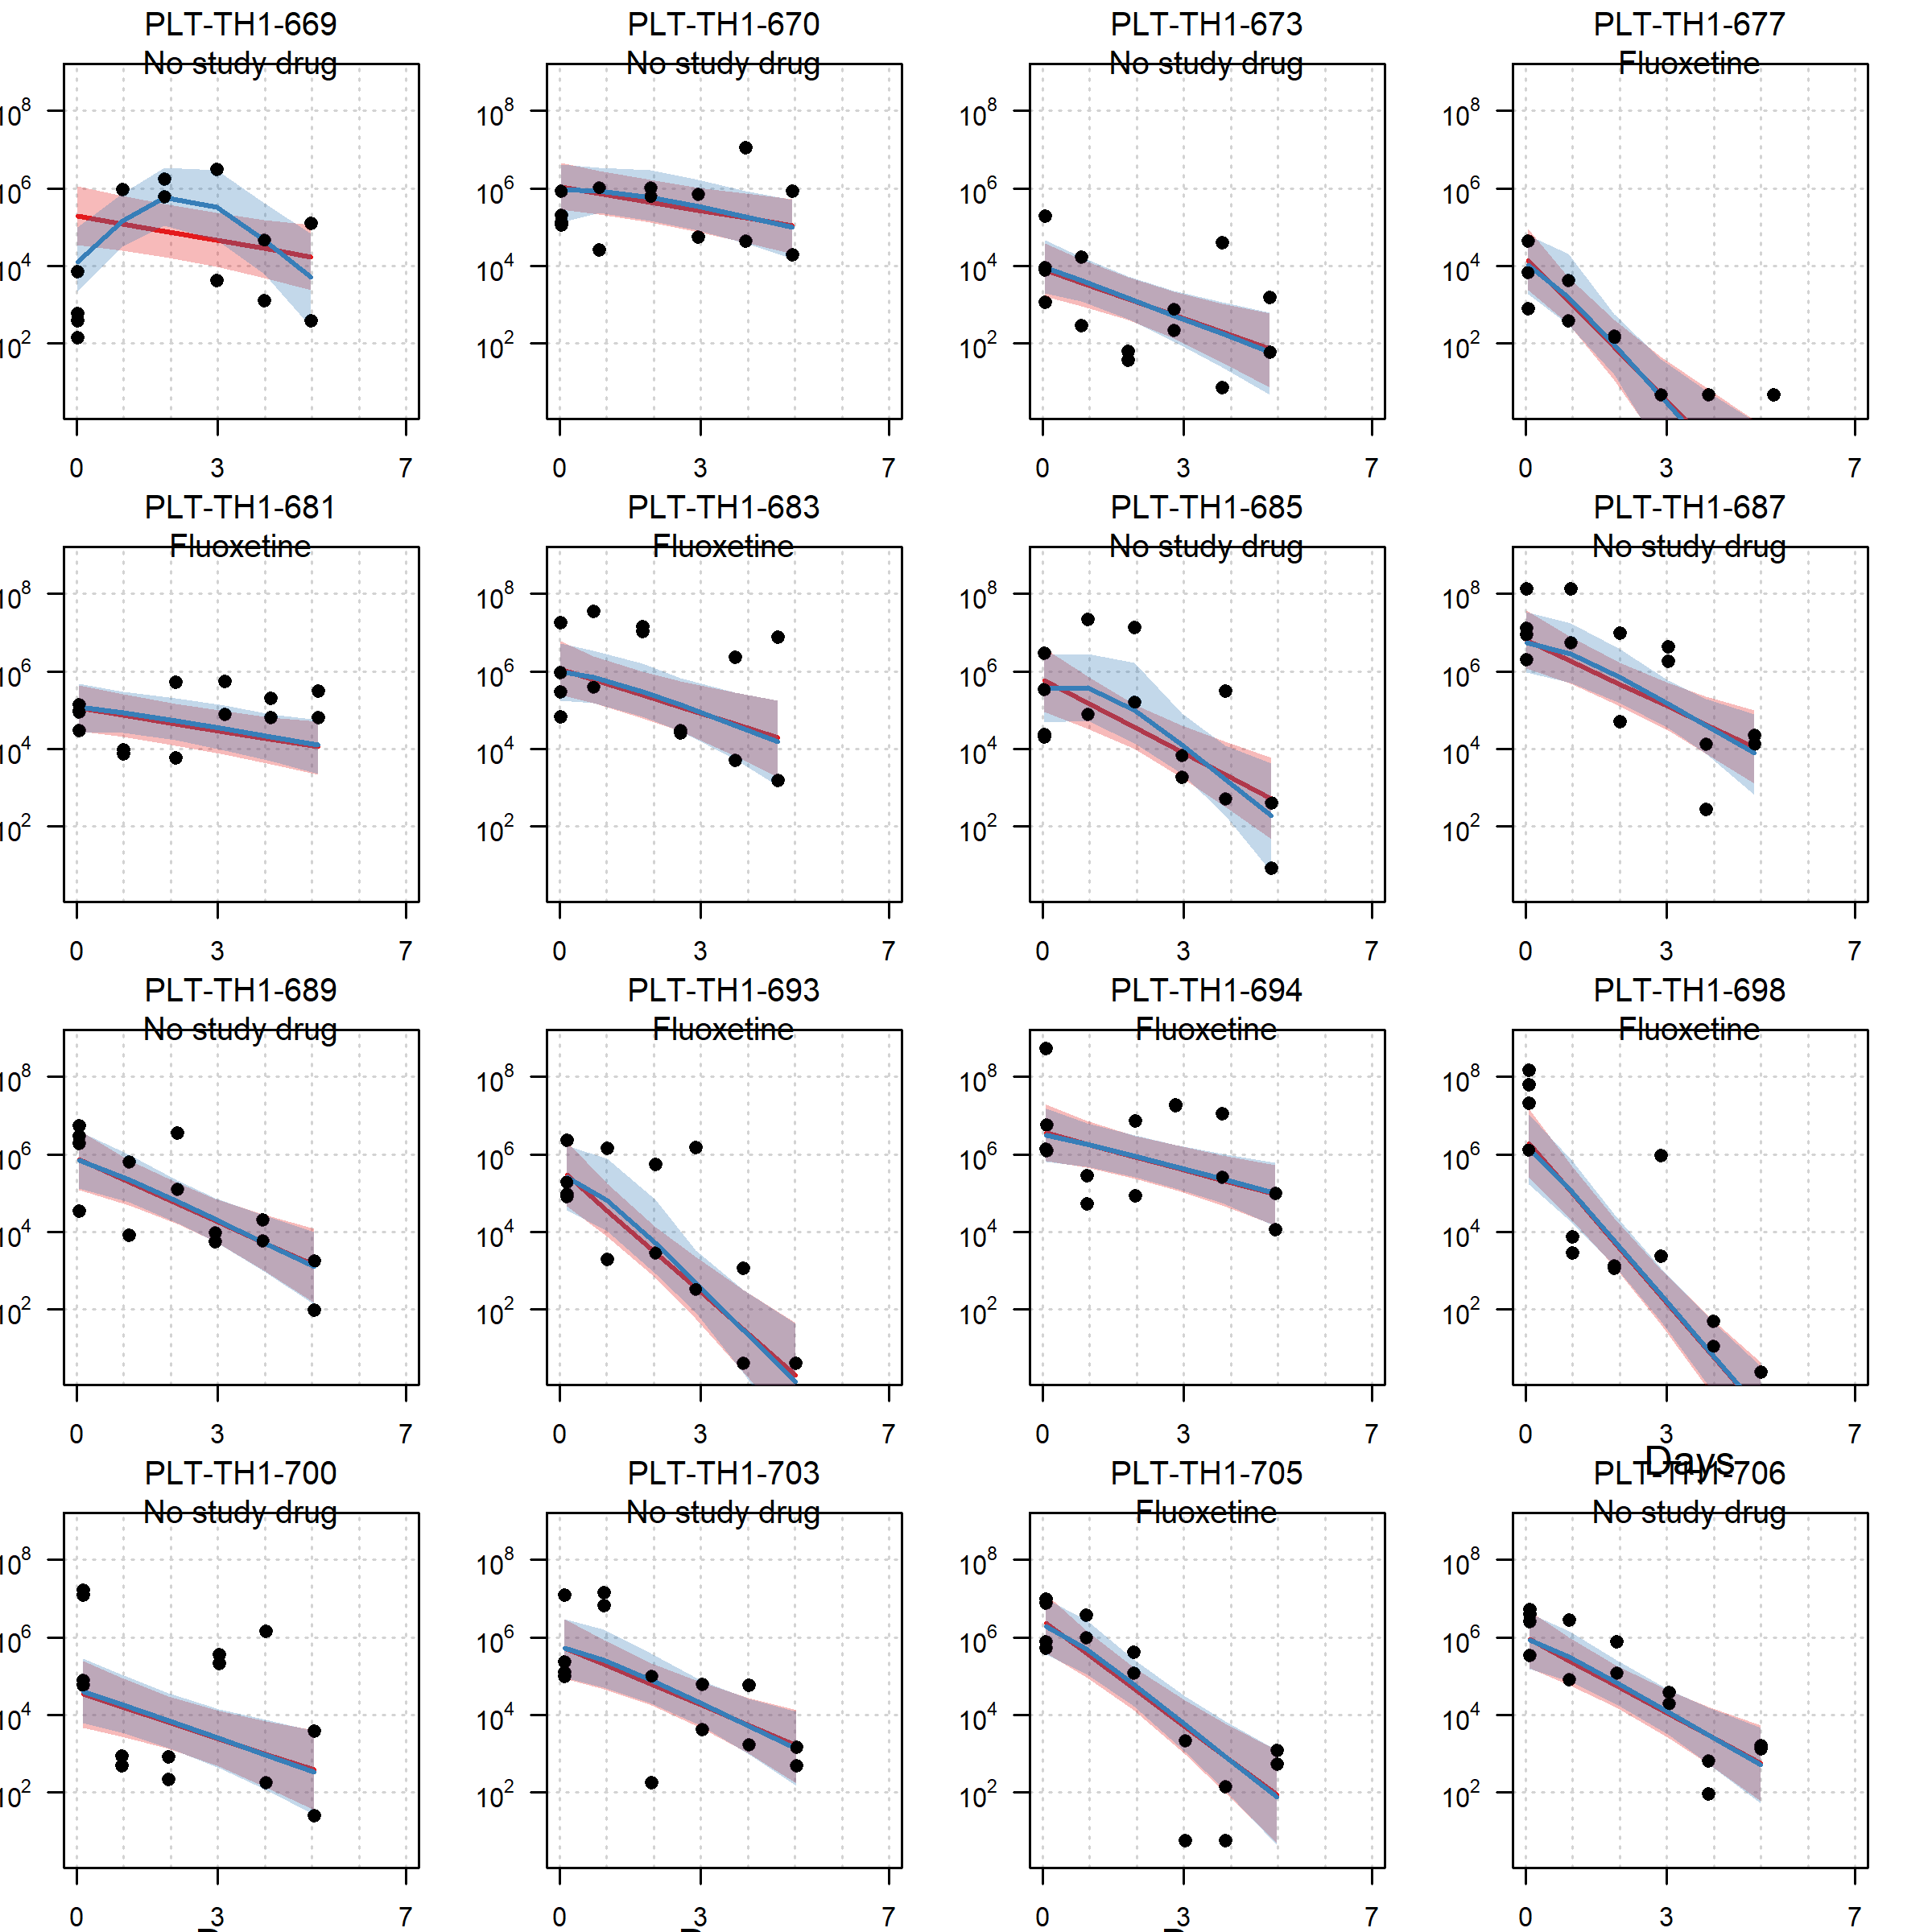
\includegraphics{Fluoxetine_analysis_files/figure-pdf/individ_data-15.png}

}

\end{figure}

\begin{figure}[H]

{\centering 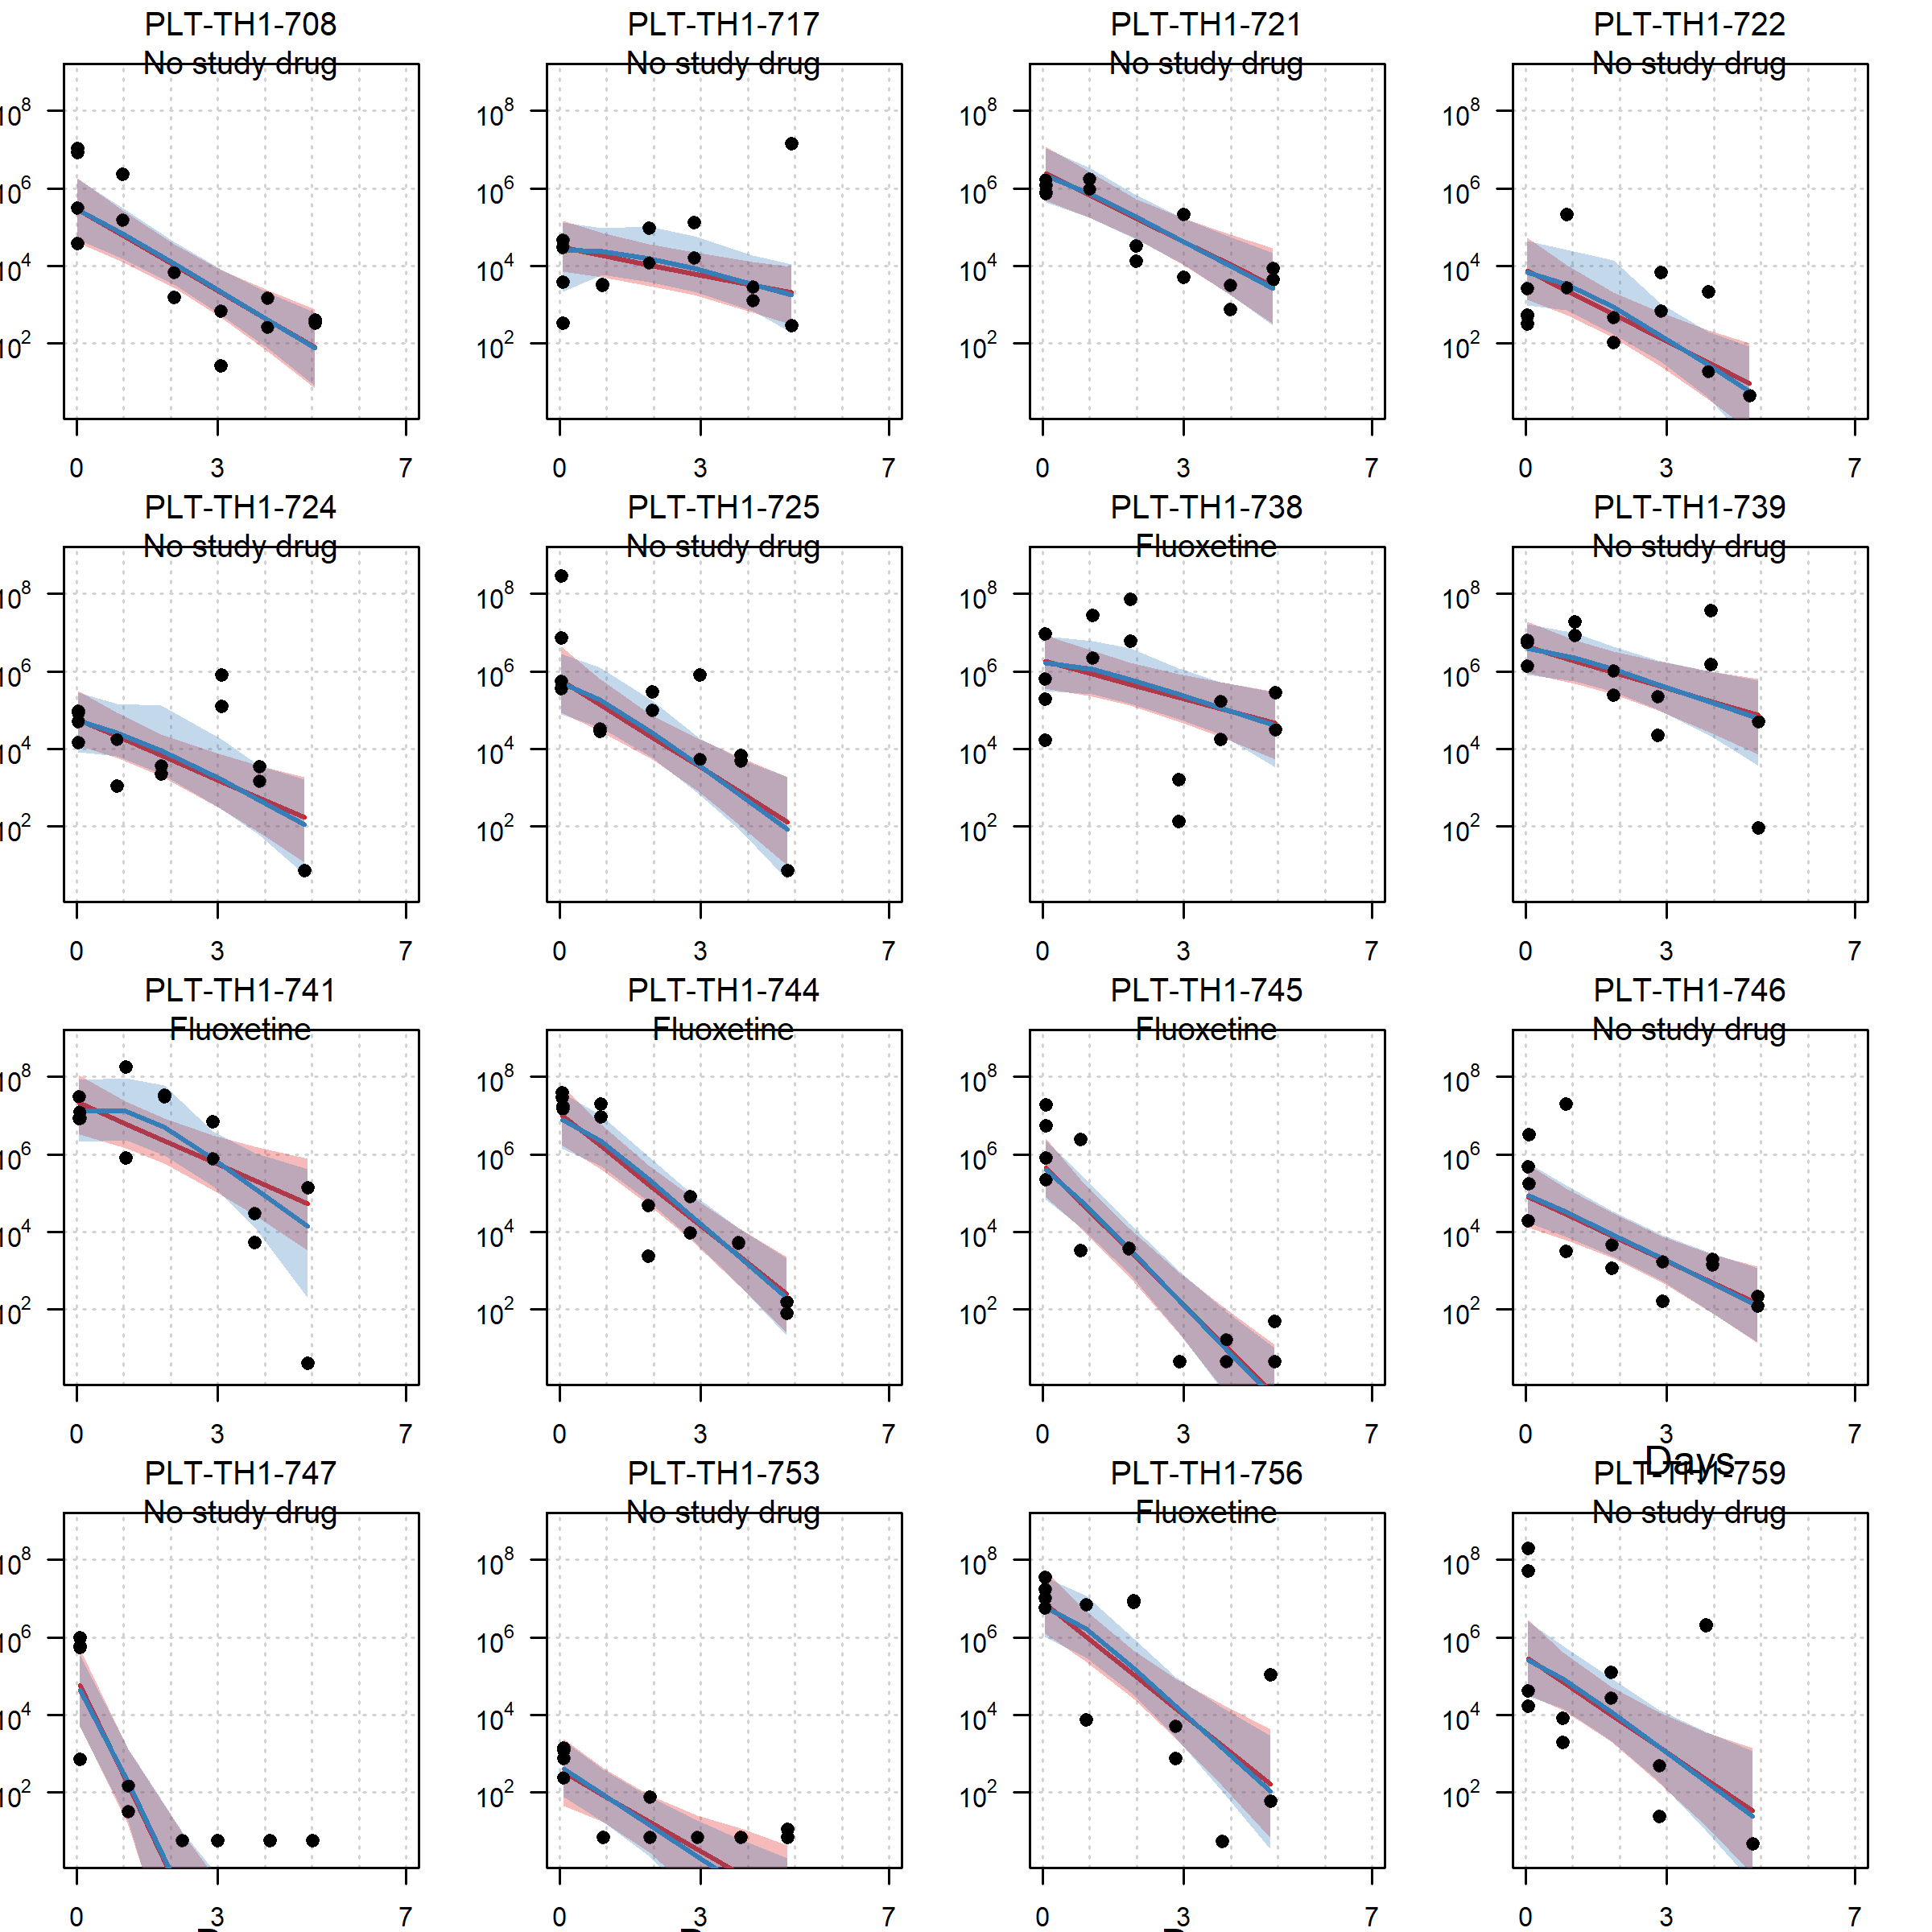
\includegraphics{Fluoxetine_analysis_files/figure-pdf/individ_data-16.png}

}

\end{figure}

\begin{figure}[H]

{\centering 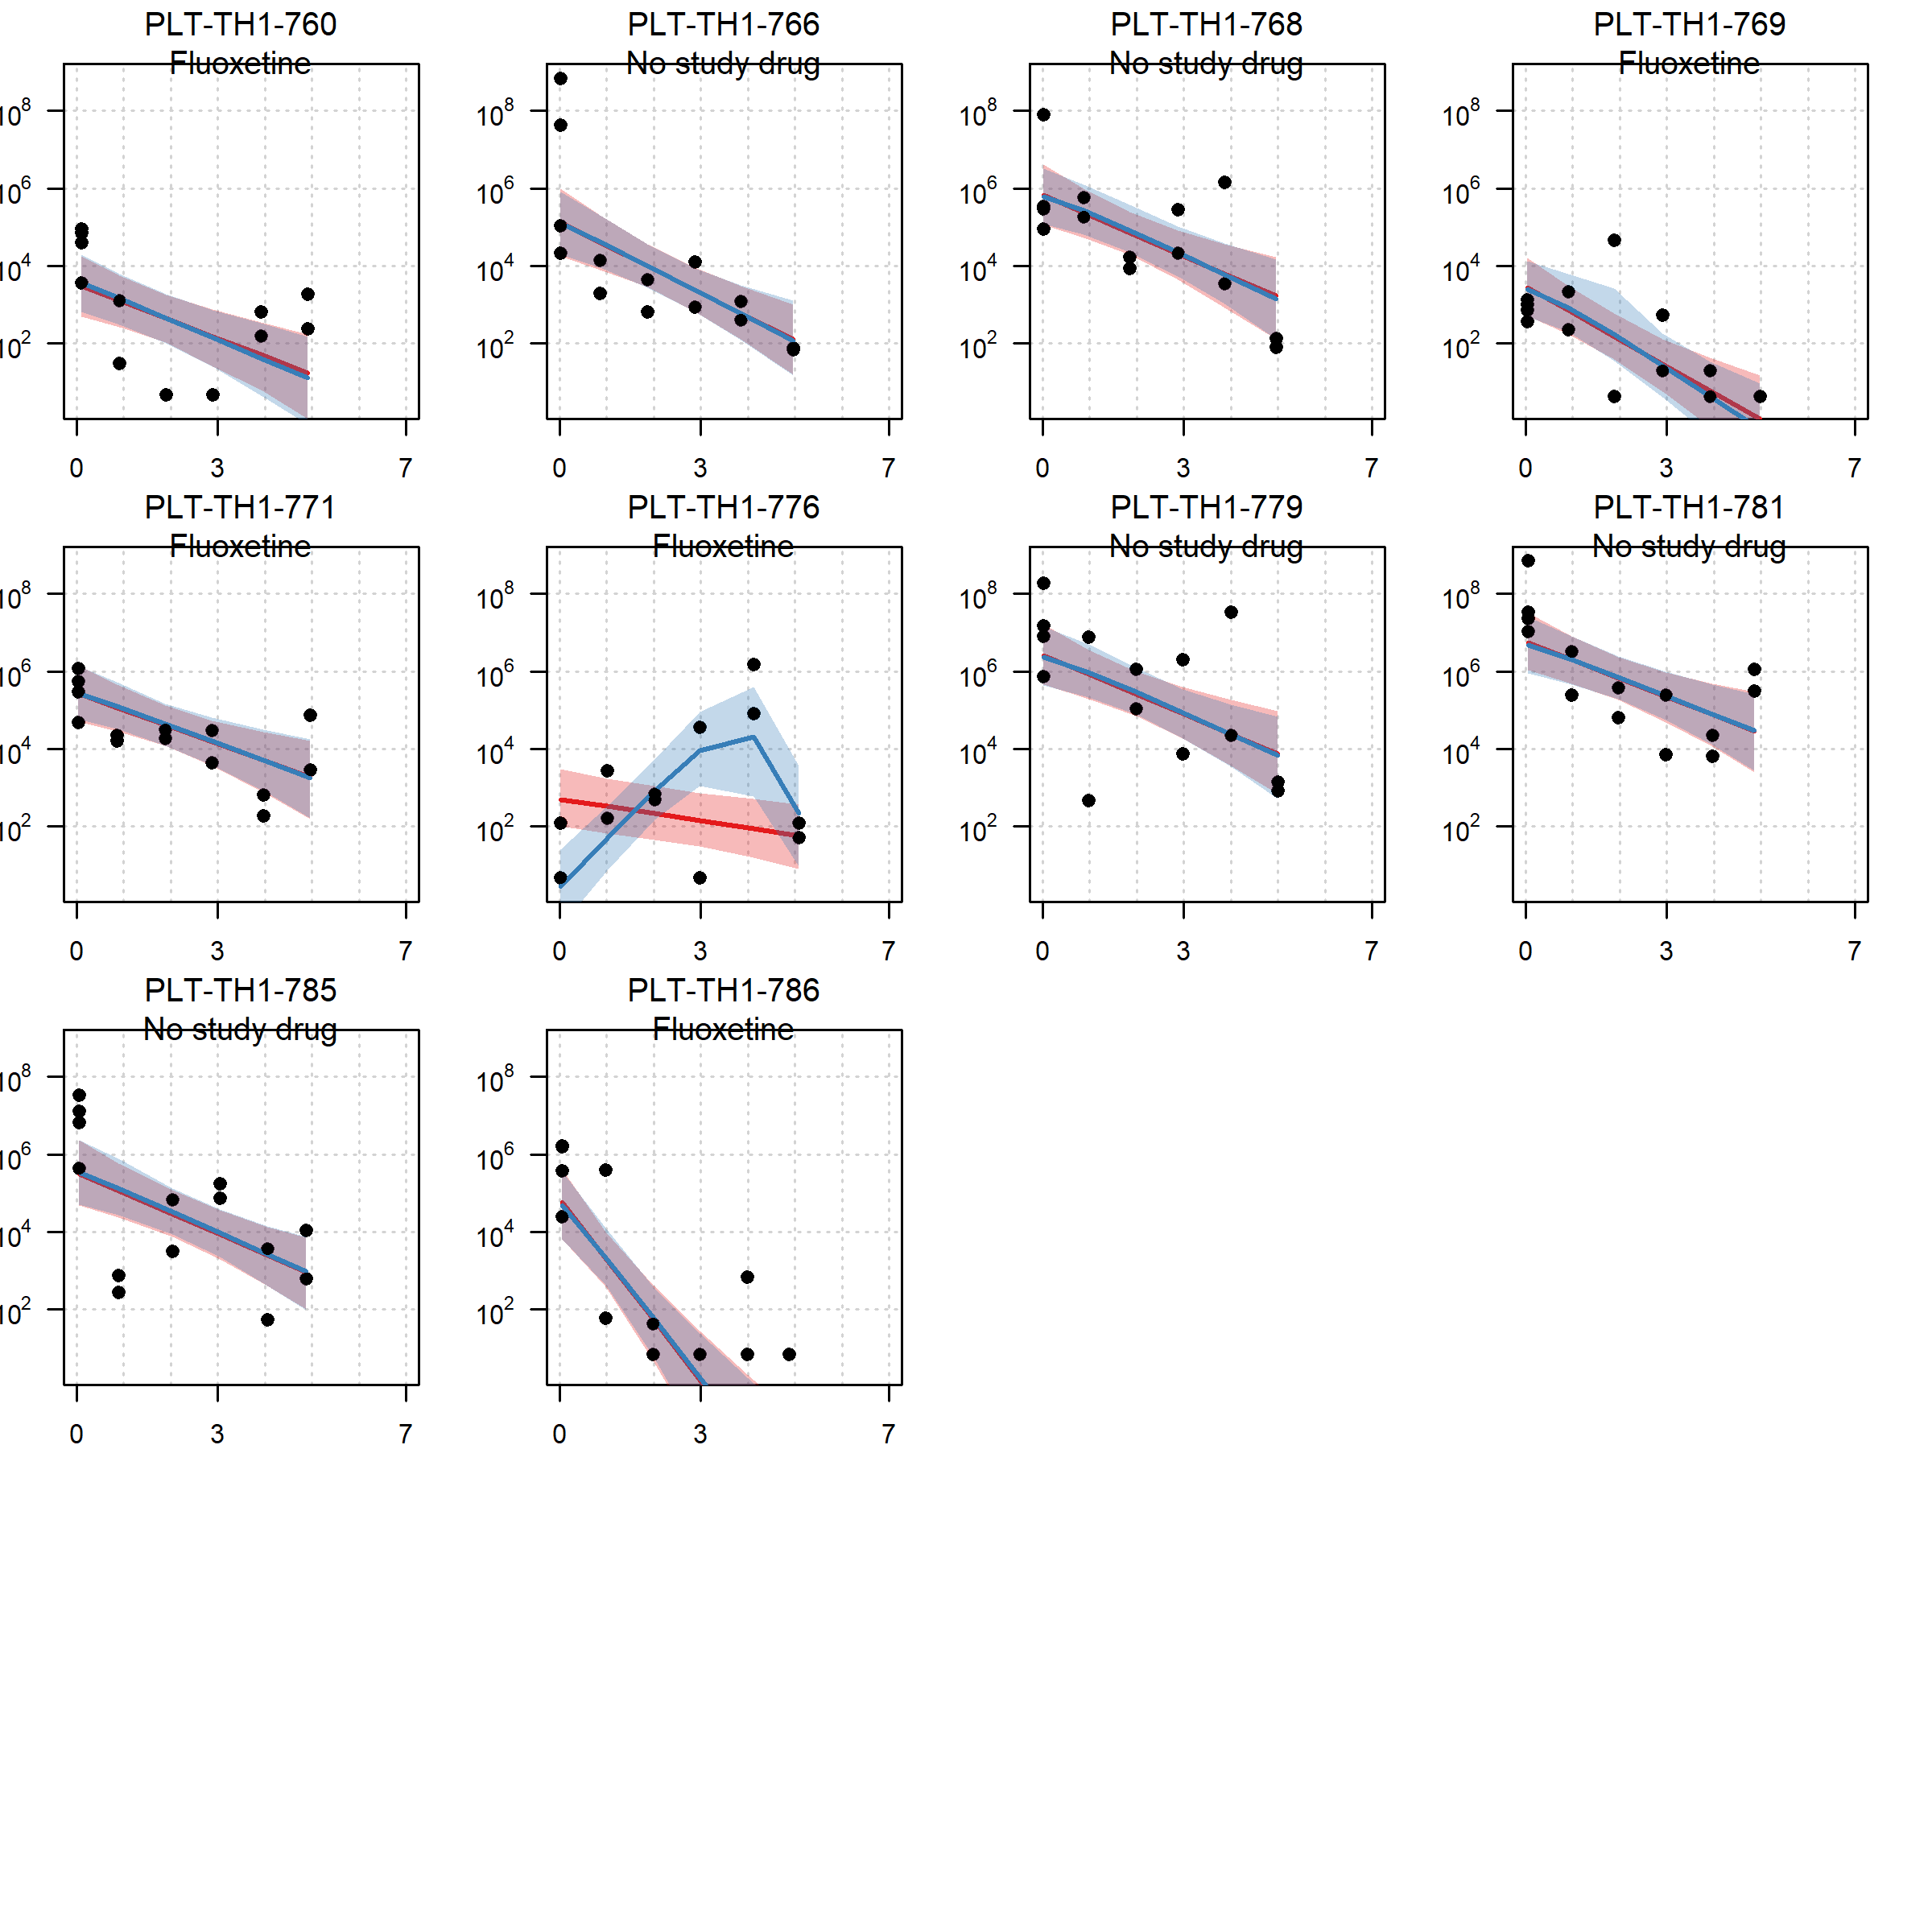
\includegraphics{Fluoxetine_analysis_files/figure-pdf/individ_data-17.png}

}

\end{figure}



\end{document}
